% Template for PLoS
% Version 3.5 March 2018
%
% % % % % % % % % % % % % % % % % % % % % %
%
% -- IMPORTANT NOTE
%
% This template contains comments intended
% to minimize problems and delays during our production
% process. Please follow the template instructions
% whenever possible.
%
% % % % % % % % % % % % % % % % % % % % % % %
%
% Once your paper is accepted for publication,
% PLEASE REMOVE ALL TRACKED CHANGES in this file
% and leave only the final text of your manuscript.
% PLOS recommends the use of latexdiff to track changes during review, as this will help to maintain a clean tex file.
% Visit https://www.ctan.org/pkg/latexdiff?lang=en for info or contact us at latex@plos.org.
%
%
% There are no restrictions on package use within the LaTeX files except that
% no packages listed in the template may be deleted.
%
% Please do not include colors or graphics in the text.
%
% The manuscript LaTeX source should be contained within a single file (do not use \input, \externaldocument, or similar commands).
%
% % % % % % % % % % % % % % % % % % % % % % %
%
% -- FIGURES AND TABLES
%
% Please include tables/figure captions directly after the paragraph where they are first cited in the text.
%
% DO NOT INCLUDE GRAPHICS IN YOUR MANUSCRIPT
% - Figures should be uploaded separately from your manuscript file.
% - Figures generated using LaTeX should be extracted and removed from the PDF before submission.
% - Figures containing multiple panels/subfigures must be combined into one image file before submission.
% For figure citations, please use "Fig" instead of "Figure".
% See http://journals.plos.org/plosone/s/figures for PLOS figure guidelines.
%
% Tables should be cell-based and may not contain:
% - spacing/line breaks within cells to alter layout or alignment
% - do not nest tabular environments (no tabular environments within tabular environments)
% - no graphics or colored text (cell background color/shading OK)
% See http://journals.plos.org/plosone/s/tables for table guidelines.
%
% For tables that exceed the width of the text column, use the adjustwidth environment as illustrated in the example table in text below.
%
% % % % % % % % % % % % % % % % % % % % % % % %
%
% -- EQUATIONS, MATH SYMBOLS, SUBSCRIPTS, AND SUPERSCRIPTS
%
% IMPORTANT
% Below are a few tips to help format your equations and other special characters according to our specifications. For more tips to help reduce the possibility of formatting errors during conversion, please see our LaTeX guidelines at http://journals.plos.org/plosone/s/latex
%
% For inline equations, please be sure to include all portions of an equation in the math environment.
%
% Do not include text that is not math in the math environment.
%
% Please add line breaks to long display equations when possible in order to fit size of the column.
%
% For inline equations, please do not include punctuation (commas, etc) within the math environment unless this is part of the equation.
%
% When adding superscript or subscripts outside of brackets/braces, please group using {}.
%
% Do not use \cal for caligraphic font.  Instead, use \mathcal{}
%
% % % % % % % % % % % % % % % % % % % % % % % %
%
% Please contact latex@plos.org with any questions.
%
% % % % % % % % % % % % % % % % % % % % % % % %

\documentclass[10pt,letterpaper]{article}
\usepackage[top=0.85in,left=2.75in,footskip=0.75in]{geometry}

% amsmath and amssymb packages, useful for mathematical formulas and symbols
\usepackage{amsmath,amssymb}

% Use adjustwidth environment to exceed column width (see example table in text)
\usepackage{changepage}

% Use Unicode characters when possible
\usepackage[utf8x]{inputenc}

% textcomp package and marvosym package for additional characters
\usepackage{textcomp,marvosym}

% cite package, to clean up citations in the main text. Do not remove.
% \usepackage{cite}

% Use nameref to cite supporting information files (see Supporting Information section for more info)
\usepackage{nameref,hyperref}

% line numbers
\usepackage[right]{lineno}

% ligatures disabled
\usepackage{microtype}
\DisableLigatures[f]{encoding = *, family = * }

% color can be used to apply background shading to table cells only
\usepackage[table]{xcolor}

% array package and thick rules for tables
\usepackage{array}

% create "+" rule type for thick vertical lines
\newcolumntype{+}{!{\vrule width 2pt}}

% create \thickcline for thick horizontal lines of variable length
\newlength\savedwidth
\newcommand\thickcline[1]{%
  \noalign{\global\savedwidth\arrayrulewidth\global\arrayrulewidth 2pt}%
  \cline{#1}%
  \noalign{\vskip\arrayrulewidth}%
  \noalign{\global\arrayrulewidth\savedwidth}%
}

% \thickhline command for thick horizontal lines that span the table
\newcommand\thickhline{\noalign{\global\savedwidth\arrayrulewidth\global\arrayrulewidth 2pt}%
\hline
\noalign{\global\arrayrulewidth\savedwidth}}


% Remove comment for double spacing
%\usepackage{setspace}
%\doublespacing

% Text layout
\raggedright
\setlength{\parindent}{0.5cm}
\textwidth 5.25in
\textheight 8.75in

% Bold the 'Figure #' in the caption and separate it from the title/caption with a period
% Captions will be left justified
\usepackage[aboveskip=1pt,labelfont=bf,labelsep=period,justification=raggedright,singlelinecheck=off]{caption}
\renewcommand{\figurename}{Fig}

% Use the PLoS provided BiBTeX style
% \bibliographystyle{plos2015}

% Remove brackets from numbering in List of References
\makeatletter
\renewcommand{\@biblabel}[1]{\quad#1.}
\makeatother



% Header and Footer with logo
\usepackage{lastpage,fancyhdr,graphicx}
\usepackage{epstopdf}
%\pagestyle{myheadings}
\pagestyle{fancy}
\fancyhf{}
%\setlength{\headheight}{27.023pt}
%\lhead{
\includegraphics[width=2.0in]{PLOS-submission.eps}}
\rfoot{\thepage/\pageref{LastPage}}
\renewcommand{\headrulewidth}{0pt}
\renewcommand{\footrule}{\hrule height 2pt \vspace{2mm}}
\fancyheadoffset[L]{2.25in}
\fancyfootoffset[L]{2.25in}
\lfoot{\today}

%% Include all macros below

\newcommand{\lorem}{{\bf LOREM}}
\newcommand{\ipsum}{{\bf IPSUM}}


% tightlist command for lists without linebreak
\providecommand{\tightlist}{%
  \setlength{\itemsep}{0pt}\setlength{\parskip}{0pt}}


% Pandoc citation processing
\newlength{\cslhangindent}
\setlength{\cslhangindent}{1.5em}
\newlength{\csllabelwidth}
\setlength{\csllabelwidth}{3em}
\newlength{\cslentryspacingunit} % times entry-spacing
\setlength{\cslentryspacingunit}{\parskip}
% for Pandoc 2.8 to 2.10.1
\newenvironment{cslreferences}%
  {}%
  {\par}
% For Pandoc 2.11+
\newenvironment{CSLReferences}[2] % #1 hanging-ident, #2 entry spacing
 {% don't indent paragraphs
  \setlength{\parindent}{0pt}
  % turn on hanging indent if param 1 is 1
  \ifodd #1
  \let\oldpar\par
  \def\par{\hangindent=\cslhangindent\oldpar}
  \fi
  % set entry spacing
  \setlength{\parskip}{#2\cslentryspacingunit}
 }%
 {}
\usepackage{calc}
\newcommand{\CSLBlock}[1]{#1\hfill\break}
\newcommand{\CSLLeftMargin}[1]{\parbox[t]{\csllabelwidth}{#1}}
\newcommand{\CSLRightInline}[1]{\parbox[t]{\linewidth - \csllabelwidth}{#1}\break}
\newcommand{\CSLIndent}[1]{\hspace{\cslhangindent}#1}

\usepackage[font=small,skip=0pt]{caption}
\usepackage{amsmath}
\usepackage[makeroom]{cancel}
\usepackage{pdflscape}
\usepackage{booktabs}
\usepackage{longtable}
\usepackage{array}
\usepackage{multirow}
\usepackage{wrapfig}
\usepackage{float}
\usepackage{colortbl}
\usepackage{pdflscape}
\usepackage{tabu}
\usepackage{threeparttable}
\usepackage{threeparttablex}
\usepackage[normalem]{ulem}
\usepackage{makecell}
\usepackage{xcolor}
\usepackage{caption}
\usepackage{graphicx}
\usepackage{siunitx}
\usepackage{hhline}
\usepackage{calc}
\usepackage{tabularx}
\usepackage{adjustbox}
\usepackage{hyperref}


\usepackage{forarray}
\usepackage{xstring}
\newcommand{\getIndex}[2]{
  \ForEach{,}{\IfEq{#1}{\thislevelitem}{\number\thislevelcount\ExitForEach}{}}{#2}
}

\setcounter{secnumdepth}{0}

\newcommand{\getAff}[1]{
  \getIndex{#1}{SEES,UoTS,CIV}
}

\begin{document}
\vspace*{0.2in}


% Title must be 250 characters or less.
\begin{flushleft}
{\Large
\textbf\newline{Introducing spatial availability, a singly-constrained
measure of competitive
accessibility} % Please use "sentence case" for title and headings (capitalize only the first word in a title (or heading), the first word in a subtitle (or subheading), and any proper nouns).
}
\newline
% Insert author names, affiliations and corresponding author email (do not include titles, positions, or degrees).
\\
Anastasia Soukhov\textsuperscript{\getAff{SEES}}\textsuperscript{*},
Antonio Paez\textsuperscript{\getAff{SEES}},
Christopher D. Higgins\textsuperscript{\getAff{UoTS}},
Moataz Mohamed\textsuperscript{\getAff{CIV}}\\
\bigskip
\textbf{\getAff{SEES}}School of Earth, Environment and Society, McMaster
University, Hamilton, ON, L8S 4K1, Canada\\
\textbf{\getAff{UoTS}}Department of Geography \& Planning, University of
Toronto Scarborough, 1265 Military Trail, Toronto, ON M1C 1A4\\
\textbf{\getAff{CIV}}Department of Civil Engineering, McMaster
University, Hamilton, ON, L8S 4K1, Canada\\
\bigskip
* Corresponding author: soukhoa@mcmaster.ca\\
\end{flushleft}
% Please keep the abstract below 300 words
\section*{Abstract}
Accessibility indicators are widely used in transportation, urban, and
healthcare planning, among many other applications. These measures are
weighted sums of reachable opportunities from a given origin conditional
on the cost of movement, and are estimates of the potential for spatial
interaction. Over time, various proposals have been forwarded to improve
their interpretability: one of those methodological additions have been
the introduction of competition. In this paper, we focus on competition,
but first demonstrate how a widely used measure of accessibility with
congestion fails to properly match the opportunity-seeking population.
We then propose an alternative formulation of accessibility with
competition, a measure we call \emph{spatial availability}. This measure
relies on proportional allocation balancing factors (fricition of
distance and population competition) that are equivalent to imposing a
single constraint on conventional gravity-based accessibility. In other
words, the proportional allocation of opportunities results in a
\emph{spatially available opportunities} value which is assigned to each
origin that, when all origin values are summed, equals the total number
of opportunities in the region. We also demonstrate how Two-Stage
Floating Catchment Area (2SFCA) methods are equvialent to spatial
availabiltiy and can be reconceptualized as singly-constrained
accessibility. To illustrate the application of spatial availability and
compare it to other relevant measures, we use data from the 2016
Transportation Tomorrow Survey of the Greater Golden Horseshoe area in
southern Ontario, Canada. Spatial availability is an important
contribution since it clarifies the interpretation of accessibility with
competition and paves the way for future applications in equity
analysis.

% Please keep the Author Summary between 150 and 200 words
% Use first person. PLOS ONE authors please skip this step.
% Author Summary not valid for PLOS ONE submissions.

\linenumbers

% Use "Eq" instead of "Equation" for equation citations.
\newpage

\hypertarget{sec:introduction}{%
\section{Introduction}\label{sec:introduction}}

The concept of accessibility in transportation studies derives its
appeal from the combination of the spatial distribution of opportunities
and the cost of reaching them {[}1,2{]}. Accessibility analysis is
employed in transportation, geography, public health, and many other
areas, with the number of applications growing {[}3{]}, especially as
mobility-based planning is de-emphasized in favor of access-oriented
planning {[}4--7{]}.

Accessibility analysis stems from the foundational works of {[}8{]} and
{[}1{]}. From these seminal efforts, many accessibility measures have
been derived, particularly after the influential work of {[}9{]} on
spatial interaction\footnote{Utility-based measures derive from a very
  different theoretical framework, random utility maximization}. Of
these, gravity-type accessibility is arguably the most common; since its
introduction in the literature, it has been widely adopted in numerous
forms {[}10--15{]}. Hansen-type accessibility indicators are essentially
weighted sums of opportunities, with the weights given by an impedance
function that depends on the cost of movement, and thus measure the
\emph{intensity of the possibility of interaction} {[}1{]}. This type of
accessibility analysis offers a powerful tool to study the intersection
between urban structure and transportation infrastructure {[}2{]}.

Despite their usefulness, the interpretability of Hansen-type
accessibility measures can be challenging {[}12,16{]}. Since they
aggregate opportunities, the results are sensitive to the size of the
region of interest (e.g., a large city has more jobs than a smaller
city). As a consequence, raw outputs are not necessarily comparable
across study areas {[}17{]}. This limitation becomes evident when
surveying studies that implement this type of analysis. For example,
{[}18{]} (in Montreal) and {[}19{]} (in Nairobi) report accessibility as
the number of health care facilities that can potentially be reached
from origins. But what does it mean for a zone to have accessibility to
less than 100 facilities in each of these two cities, with their
different populations and number of facilities? For that matter, what
does it mean for a zone to have accessibility to more than 700
facilities in Montreal, besides being ``accessibility rich''? As another
example, {[}20{]} (in Bogota), {[}21{]} (in Montreal), and {[}22{]} (in
Beijing) report accessibility as numbers of jobs, with accessibility
values often in the hundreds of thousands, and even exceeding one
million jobs for some zones in Beijing and Montreal. As indicators of
urban structure, these measures are informative, but the meaning of one
million accessible jobs is harder to pin down: how many jobs must any
single person have access to? Clearly, the answer to this question
depends on how many people demand jobs.

The interpretability of Hansen-type accessibility has been discussed in
numerous studies, including recently by {[}23{]}, {[}24{]}, and in
greater depth by {[}25{]}. As hinted above, the limitations in
interpretability are frequently caused by ignoring competition - without
competition, each opportunity is assumed to be equally available to
every single opportunity-seeking individual that can reach it
{[}24,26,27{]}. This assumption is appropriate when the opportunity of
interest is non-exclusive, that is, if use by one unit of population
does not preclude use by another. For instance, national parks with
abundant space are seldom used to full capacity, so the presence of some
population does not exclude use by others. When it comes to exclusive
opportunities, or when operations may be affected by congestion, the
solution has been to account for competition. Several efforts exist that
do so. In our reckoning, the first such approach was proposed by
{[}28{]}, whereby the distance decay of the supply of employment and the
demand for employment (by workers) were formulated under so-called
axiomatic assumptions. This approach was then applied by {[}29{]} in the
context of healthcare, to quantify the availability of general
practitioners in Canada. About two decades later, {[}26{]} independently
re-discovered Weibull's {[}28{]} formula {[}see footnote (7) in 26{]}
and deconstructed it to consider accessibility for different modes.
These advances were subsequently popularized as the family of Two-Stage
Floating Catchment area (2SFCA) methods {[}30{]} that have found
widespread adoption in healthcare, education, and food systems
{[}31--35{]}.

An important development contained in Shen's work is a proof that the
population-weighted sum of the accessibility measure with competition
equates to the number of opportunities available {[}footnote (7) and
Appendix A in 26{]}. This demonstration gives the impression that
Shen-type accessibility allocates \emph{all} opportunities to the
origins, however to the authors' knowledge, it has not interpreted by
literature in this way. For instance, {[}36{]}, {[}25{]}, and {[}37{]}
all use Shen-type accessibility to calculate job access but report
values as `competitive accessibility scores' or simply `job
accessibility'. These works do not explicitly recognize that jobs that
are assigned to each origin are in fact a proportion of \emph{all} the
opportunities in the system. This recognition, we argue, is critical to
interpreting the meaning of the final result. Thus, in this paper we
intend to revisit accessibility with competition within the context of
disentangling how opportunities are allocated. We first argue that
Shen's competitive accessibility misleadingly refers to the the total
zonal population to equal the travel-cost discounted opportunity-seeking
population. This equivocation, we believe, results in a ambigious
interpretation of what Shen-type accessibility represents as the
allocation of opportunities to population is masked by the results
presenting as rates (i.e., opportunities per capita). We then propose an
alternative formulation of accessibility that incorporates competition
by adopting a proportional allocation mechanism; we name this measure
\emph{spatial availability}. The use of balancing factors for
proportional allocation is akin to imposing a single constraint on the
accessibility indicator, in the spirit of Wilson's {[}9{]} spatial
interaction model.

The key motivations of this paper are as follows:

\begin{itemize}
\item
  To address and improve on the interpretability of Hansen-type
  accessibility measure; and
\item
  To consider competition from the perspective of the population for
  opportunities within an accessibility measure.
\end{itemize}

In this way, the paper's aim is three-fold:

\begin{itemize}
\item
  First, we aim to demonstrate that Shen-type (and thus {[}28{]}
  accessibility and the popular 2SFCA methods) produce equivocal
  estimates of opportunities allocated as the result is presented as a
  rate (i.e., opportunities per capita);
\item
  Second, we introduce a new measure, \emph{spatial availability}, which
  we submit is a more interpretable alternative to Shen-type
  accessibility, since opportunities in the system are preserved and
  proportionally allocated to the population; and
\item
  Third, we show how Shen-type accessibility (and 2SFCA methods) can be
  seen as measures of singly-constrained accessibility.
\end{itemize}

Discussion is supported by the use of the small synthetic example of
{[}26{]} and empirical data drawn from the 2016 Transportation Tomorrow
Survey of the Greater Toronto and Hamilton Area in Ontario, Canada. In
the spirit of openness of research in the spatial sciences {[}38,39{]}
this paper has a companion open data product {[}40{]}, and all code is
available for replicability and reproducibility purposes at
\url{https://github.com/soukhova/Spatial-Availability-Measure}.

\hypertarget{background}{%
\section{Accessibility measures revisited}\label{background}}

In this section we revisit Hansen-type and Shen-type accessibility
indicators. We adopt the convention of using a capital letter for
absolute values (number of opportunities) and lower case for rates
(opportunities per capita).

\hypertarget{hansen-type-accessibility}{%
\subsection{Hansen-type accessibility}\label{hansen-type-accessibility}}

Hansen-type accessibility measures follow the general formulation shown
in Equation (\ref{eq:conventional-accessibility}):

\begin{equation}
\label{eq:conventional-accessibility}
S_i = \sum_{j=1}^JO_j \cdot f(c_{ij})
\end{equation}

\noindent where:

\begin{itemize}
\tightlist
\item
  \(c_{ij}\) is a measure of the cost of moving between \(i\) and \(j\).
\item
  \(f(\cdot)\) is an impedance function of \(c_{ij}\); it can take the
  form of any monotonically decreasing function chosen based on positive
  or normative criteria {[}41{]}.
\item
  \(i\) is a set of origin locations (\(i = 1,\cdots,N\)).
\item
  \(j\) is a set of destination locations (\(j = 1,\cdots,J\)).
\item
  \(O_j\) is the number of opportunities at location \(j\);
  \(O = \sum_{j=1}^J O_j\) is the total supply of opportunities in the
  study region.
\item
  \(S\) is Hansen-type accessibility as weighted sum of opportunities.
\end{itemize}

As formally defined, accessibility \(S_i\) is the sum of opportunities
that can be reached from location \(i\), weighted down by an impedance
function of the cost of travel \(c_{ij}\). Summing the opportunities in
the neighborhood of \(i\) provides estimates of the number of
opportunities that can \emph{potentially} be reached from \(i\). Several
measures result from using a variety of impedance functions; for
example, cumulative opportunities measures are obtained when
\(f(\cdot)\) is a binary or indicator function {[}12,e.g., 21,42,43{]}.
Other measures use impedance functions modeled after any monotonically
decreasing function {[}e.g., Gaussian, inverse power, negative
exponential, or log-normal, among others, see, \emph{inter alia},
44,45--47{]}. In practice, accessibility measures with different
impedance functions tend to be highly correlated {[}44,48,49{]}.

Gravity-based accessibility has been shown to be an excellent indicator
of the intersection between spatially distributed opportunities and
transportation infrastructure {[}3,44,46{]}. However, beyond enabling
comparisons of relative values they are not highly interpretable on
their own {[}16{]}. To address the issue of interpretability, previous
research has aimed to index and normalize values on a per
demand-population basis {[}e.g., 50,51,52{]}. However, as recent
research on accessibility discusses {[}17,24,e.g., 25,27{]}, these steps
do not adequately consider competition. In effect, when calculating
\(S_i\), every opportunity enters the weighted sum once for every origin
\(i\) that can reach it. This makes interpretability opaque, and to
complicate matters, can also bias the estimated landscape of
opportunity.

\hypertarget{shen-type-competitive-accessibility}{%
\subsection{Shen-type competitive
accessibility}\label{shen-type-competitive-accessibility}}

To account for competition, the influential works of {[}26{]} and
{[}28{]}, as well as the widely used 2SFCA approach of {[}30{]}, adjust
Hansen-type accessibility with the population in the region of interest.
The mechanics of this approach consist of calculating, for every
destination \(j\), the population that can reach it given the impedance
function \(f(\cdot)\); let us call this the \emph{effective
opportunity-seeking population} (Equation
(\ref{eq:effective-opportunity-seeking-population})). This value can be
seen as the Hansen-type \emph{market area} (accessibility to population)
of \(j\). The opportunities at \(j\) are then divided by the sum of the
effective opportunity-seeking population to obtain a measure of
opportunities per capita, i.e., \(R_j\) in Equation
(\ref{eq:level-of-service}). This can be thought of as the \emph{level
of service} at \(j\). Per capita values are then allocated back to the
population at \(i\), again subject to the impedance function as seen in
Equation (\ref{eq:2SFCA-step2}); this is accessibility with competition.

\begin{equation}
\label{eq:effective-opportunity-seeking-population}
P_{ij}^{*} = {P_{i} \cdot f(c_{ij})}
\end{equation}

\begin{equation}
\label{eq:level-of-service}
R_{j} = \frac{O_{j}}{\sum_i P_{ij}^*}
\end{equation}

\begin{equation}
\label{eq:2SFCA-step2}
a_{i} = {\sum_j R_{j} \cdot f(c_{ij})}
\end{equation}

\noindent where:

\begin{itemize}
\tightlist
\item
  \(a\) is Shen-type accessibility as weighted sum of opportunities per
  capita (or weighted level of service).
\item
  \(c_{ij}\) is a measure of the cost of moving between \(i\) and \(j\).
\item
  \(f(\cdot)\) is an impedance function of \(c_{ij}\).
\item
  \(i\) is a set of origin locations (\(i = 1,\cdots,N\)).
\item
  \(j\) is a set of destination locations (\(j = 1,\cdots,J\)).
\item
  \(O_j\) is the number of opportunities at location \(j\);
  \(O = \sum_{j=1}^J O_j\) is the total supply of opportunities in the
  study region.
\item
  \(P_i\) is the population at location \(i\).
\item
  \(P_{ij}^*\) is the population at location \(i\) that can reach
  destination \(j\) according to the impedance function; we call this
  the \emph{effective opportunity-seeking population}.
\item
  \(R_j\) is the ratio of opportunities at \(j\) to the sum over all
  origins of the \emph{effective opportunity-seeking population} that
  can reach \(j\); in other words, this is the total number of
  opportunities per capita found at \(j\).
\end{itemize}

{[}26{]} describes \(P_i\) as the \emph{``the number of people in
location \(i\) seeking opportunities''}. In our view, this is somewhat
equivocal and where misinterpretation of the final results may arise.
Consider a population center where the population is only willing to
take an opportunity if the trip required is less than or equal to 60
minutes. This is identical to the following impedance function:

\begin{equation}
\label{eq:binary-impedance}
f(c_{ij}) =
\begin{cases}
1\text{ if }c_{ij}\leq60\text{ min}\\
0\text{ otherwise}\\
\end{cases}
\end{equation}

If an employment center is less than 60 minutes away, the population can
seek opportunities there (i.e., \(f(c_{ij})=1\)). But are these people
still part of the opportunity-seeking population for jobs located two
hours away? Four hours? Ten hours? We assume that they are not because
their travel behaviour, as represented by the impedance function would
yield \(f(c_{ij})=0\), eliminating them from the effective
opportunity-seeking population \(P_ij*\). We see Shen's definition as
ambiguous because, for the purpose of calculating accessibility, the
impedance function defines what constitutes the population that
effectively can seek opportunities at remote locations. Thus \(P_i\)
should be plainly understood as the population at location \(i\) (as
defined above) and not the \emph{``the number of people in location
\(i\) seeking opportunities''}. In other words, \(P_i\) and \(P_{ij}*\)
are confounded.

Furthermore, an identical misunderstanding can be described for \(O_j\)
which is defined as \emph{``the number of \textbf{relevant}
opportunities in location j''} in {[}26{]} (our emphasis). \(O_j\) is
adjusted by the same \(f(c_{ij})\) in Equation (\ref{eq:2SFCA-step2}),
so the \emph{relevancy} is determined by the travel behaviour associated
with the impedance function not purely by \(O_j\) itself. For this
reason, \(O_j\) should be understand plainly as the opportunities at
location \(j\) (as we also defined them above).

Misunderstanding \(P_i\) and \(O_j\) may lead to a misleading
interpretation of the final result \(a_i\), especially as expressed in
Shen's proof (see Equation (\ref{eq:2SFCA-total})).

\begin{equation}
\label{eq:2SFCA-total}
\sum_{i=1}^N a_{i} P_i= \sum_{j=1}^JO_j
\end{equation}

Notice, confounding \(P_i\) with the effective opportunity-seeking
population and \(O_j\) with the jobs taken may cause us to misunderstand
\(a_{i}\) as \emph{``relevant opportunities''} per \emph{``people in
location \(i\) seeking opportunities''}. Instead, as mathematically
expressed in the proof, \(a_{i}\) is a proportion of the opportunities
available to the population, since multiplying \(a_i\) by the population
at \(i\) and summing for all origins in the system equals to the total
number of opportunities in the system. Embedded in \(a_i\) is already
the travel behaviour so \(P_i\) and \(O_j\) must be plainly understand
as population at \(i\) and opportunities at \(j\) to have Equation
(\ref{eq:2SFCA-total}) hold true.

\hypertarget{shens-synthetic-example}{%
\subsection{Shen's synthetic example}\label{shens-synthetic-example}}

In this section we use the example in {[}26{]} to detail the importance
of understanding \(P_i\) and \(O_j\) as simply the population at the
origin \(i\) and the opportunities at destination \(j\) respectively.
This is critical to understanding how the opportunities are allocated to
the population based on the impedance function.

\begin{figure}

{\centering 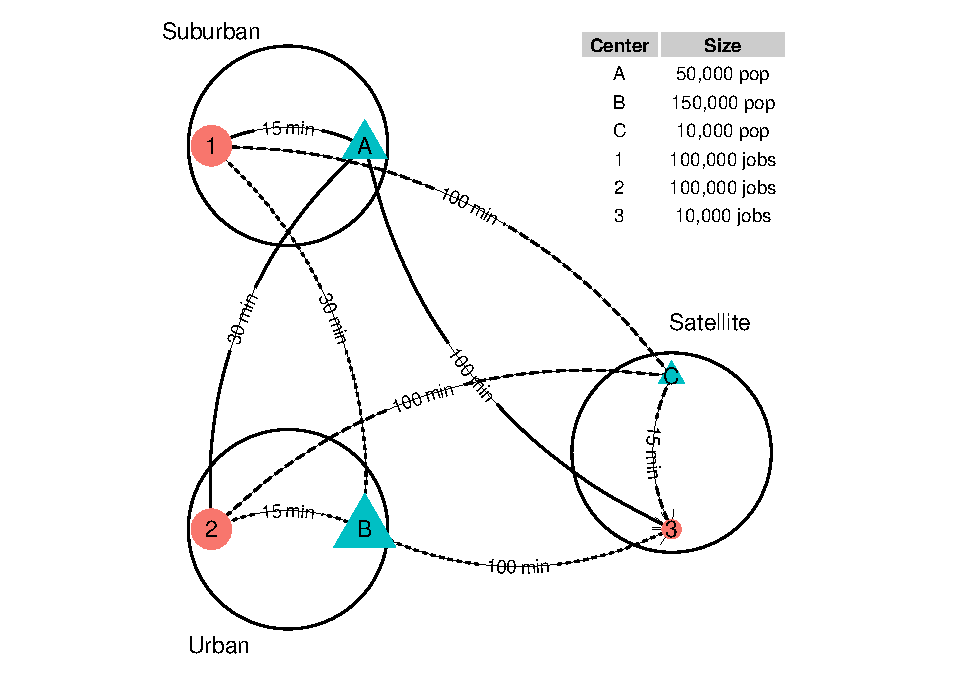
\includegraphics[width=1\linewidth]{Spatial-Availability-Refreshed_files/figure-latex/create-figure-with-toy-example-1} 

}

\caption{\label{fig:plot-toy-example} Shen (1998) synthetic example with locations of employment centers (in orange), population centers (in blue), number of jobs and population, and travel times.}\label{fig:create-figure-with-toy-example}
\end{figure}

 
  \providecommand{\huxb}[2]{\arrayrulecolor[RGB]{#1}\global\arrayrulewidth=#2pt}
  \providecommand{\huxvb}[2]{\color[RGB]{#1}\vrule width #2pt}
  \providecommand{\huxtpad}[1]{\rule{0pt}{#1}}
  \providecommand{\huxbpad}[1]{\rule[-#1]{0pt}{#1}}

\begin{table}[h!]
\begin{centerbox}
\begin{threeparttable}
\captionsetup{justification=centering,singlelinecheck=off}
\caption{Summary description of synthetic example: Hansen-type accessibility $S_i$, Shen-type accessibility $a_i$, and spatial availability $V_i$ with beta = 0.1 (light yellow) and beta = 0.6 (light grey).}
 \label{tab:synthetic-example}
\setlength{\tabcolsep}{0pt}
\begin{tabularx}{1.1\textwidth}{p{0.11\textwidth} p{0.11\textwidth} p{0.11\textwidth} p{0.11\textwidth} p{0.11\textwidth} p{0.11\textwidth} p{0.11\textwidth} p{0.11\textwidth} p{0.11\textwidth} p{0.11\textwidth}}


\hhline{>{\huxb{190, 190, 190}{1}}|>{\huxb{190, 190, 190}{1}}|>{\huxb{190, 190, 190}{1}}|>{\huxb{190, 190, 190}{1}}|}
\arrayrulecolor{black}

\multicolumn{1}{!{\huxvb{0, 0, 0}{0}}p{0.11\textwidth}!{\huxvb{190, 190, 190}{1}}}{\hspace{6pt}\parbox[b]{0.11\textwidth-6pt-6pt}{\huxtpad{6pt + 1em}\raggedright \textbf{{\fontsize{7pt}{8.4pt}\selectfont Origin}}\huxbpad{6pt}}} &
\multicolumn{3}{p{0.33\textwidth+4\tabcolsep}!{\huxvb{190, 190, 190}{1}}}{\hspace{6pt}\parbox[b]{0.33\textwidth+4\tabcolsep-6pt-6pt}{\huxtpad{6pt + 1em}\centering \textbf{{\fontsize{7pt}{8.4pt}\selectfont A}}\huxbpad{6pt}}} &
\multicolumn{3}{p{0.33\textwidth+4\tabcolsep}!{\huxvb{190, 190, 190}{1}}}{\hspace{6pt}\parbox[b]{0.33\textwidth+4\tabcolsep-6pt-6pt}{\huxtpad{6pt + 1em}\centering \textbf{{\fontsize{7pt}{8.4pt}\selectfont B}}\huxbpad{6pt}}} &
\multicolumn{3}{p{0.33\textwidth+4\tabcolsep}!{\huxvb{190, 190, 190}{1}}}{\hspace{6pt}\parbox[b]{0.33\textwidth+4\tabcolsep-6pt-6pt}{\huxtpad{6pt + 1em}\centering \textbf{{\fontsize{7pt}{8.4pt}\selectfont C}}\huxbpad{6pt}}} \tabularnewline[-0.5pt]


\hhline{>{\huxb{0, 0, 0}{0.4}}->{\huxb{0, 0, 0}{0.4}}->{\huxb{0, 0, 0}{0.4}}->{\huxb{0, 0, 0}{0.4}}->{\huxb{0, 0, 0}{0.4}}->{\huxb{0, 0, 0}{0.4}}->{\huxb{0, 0, 0}{0.4}}->{\huxb{0, 0, 0}{0.4}}->{\huxb{0, 0, 0}{0.4}}->{\huxb{0, 0, 0}{0.4}}-}
\arrayrulecolor{black}

\multicolumn{1}{!{\huxvb{0, 0, 0}{0}}p{0.11\textwidth}!{\huxvb{190, 190, 190}{1}}}{\hspace{6pt}\parbox[b]{0.11\textwidth-6pt-6pt}{\huxtpad{6pt + 1em}\raggedright \textbf{{\fontsize{7pt}{8.4pt}\selectfont Dest.}}\huxbpad{6pt}}} &
\multicolumn{1}{p{0.11\textwidth}!{\huxvb{0, 0, 0}{0}}}{\hspace{6pt}\parbox[b]{0.11\textwidth-6pt-6pt}{\huxtpad{6pt + 1em}\centering \textbf{{\fontsize{7pt}{8.4pt}\selectfont 1}}\huxbpad{6pt}}} &
\multicolumn{1}{p{0.11\textwidth}!{\huxvb{0, 0, 0}{0}}}{\hspace{6pt}\parbox[b]{0.11\textwidth-6pt-6pt}{\huxtpad{6pt + 1em}\centering \textbf{{\fontsize{7pt}{8.4pt}\selectfont 2}}\huxbpad{6pt}}} &
\multicolumn{1}{p{0.11\textwidth}!{\huxvb{190, 190, 190}{1}}}{\hspace{6pt}\parbox[b]{0.11\textwidth-6pt-6pt}{\huxtpad{6pt + 1em}\centering \textbf{{\fontsize{7pt}{8.4pt}\selectfont 3}}\huxbpad{6pt}}} &
\multicolumn{1}{p{0.11\textwidth}!{\huxvb{0, 0, 0}{0}}}{\hspace{6pt}\parbox[b]{0.11\textwidth-6pt-6pt}{\huxtpad{6pt + 1em}\centering \textbf{{\fontsize{7pt}{8.4pt}\selectfont 1}}\huxbpad{6pt}}} &
\multicolumn{1}{p{0.11\textwidth}!{\huxvb{0, 0, 0}{0}}}{\hspace{6pt}\parbox[b]{0.11\textwidth-6pt-6pt}{\huxtpad{6pt + 1em}\centering \textbf{{\fontsize{7pt}{8.4pt}\selectfont 2}}\huxbpad{6pt}}} &
\multicolumn{1}{p{0.11\textwidth}!{\huxvb{190, 190, 190}{1}}}{\hspace{6pt}\parbox[b]{0.11\textwidth-6pt-6pt}{\huxtpad{6pt + 1em}\centering \textbf{{\fontsize{7pt}{8.4pt}\selectfont 3}}\huxbpad{6pt}}} &
\multicolumn{1}{p{0.11\textwidth}!{\huxvb{0, 0, 0}{0}}}{\hspace{6pt}\parbox[b]{0.11\textwidth-6pt-6pt}{\huxtpad{6pt + 1em}\centering \textbf{{\fontsize{7pt}{8.4pt}\selectfont 1}}\huxbpad{6pt}}} &
\multicolumn{1}{p{0.11\textwidth}!{\huxvb{0, 0, 0}{0}}}{\hspace{6pt}\parbox[b]{0.11\textwidth-6pt-6pt}{\huxtpad{6pt + 1em}\centering \textbf{{\fontsize{7pt}{8.4pt}\selectfont 2}}\huxbpad{6pt}}} &
\multicolumn{1}{p{0.11\textwidth}!{\huxvb{190, 190, 190}{1}}}{\hspace{6pt}\parbox[b]{0.11\textwidth-6pt-6pt}{\huxtpad{6pt + 1em}\centering \textbf{{\fontsize{7pt}{8.4pt}\selectfont 3}}\huxbpad{6pt}}} \tabularnewline[-0.5pt]


\hhline{>{\huxb{0, 0, 0}{0.4}}->{\huxb{0, 0, 0}{0.4}}->{\huxb{0, 0, 0}{0.4}}->{\huxb{0, 0, 0}{0.4}}->{\huxb{0, 0, 0}{0.4}}->{\huxb{0, 0, 0}{0.4}}->{\huxb{0, 0, 0}{0.4}}->{\huxb{0, 0, 0}{0.4}}->{\huxb{0, 0, 0}{0.4}}->{\huxb{0, 0, 0}{0.4}}-}
\arrayrulecolor{black}

\multicolumn{1}{!{\huxvb{0, 0, 0}{0}}p{0.11\textwidth}!{\huxvb{190, 190, 190}{1}}}{\hspace{6pt}\parbox[b]{0.11\textwidth-6pt-6pt}{\huxtpad{6pt + 1em}\raggedright {\fontsize{7pt}{8.4pt}\selectfont Pop.}\huxbpad{6pt}}} &
\multicolumn{1}{p{0.11\textwidth}!{\huxvb{0, 0, 0}{0}}}{\hspace{6pt}\parbox[b]{0.11\textwidth-6pt-6pt}{\huxtpad{6pt + 1em}\centering {\fontsize{7pt}{8.4pt}\selectfont  50000}\huxbpad{6pt}}} &
\multicolumn{1}{p{0.11\textwidth}!{\huxvb{0, 0, 0}{0}}}{\hspace{6pt}\parbox[b]{0.11\textwidth-6pt-6pt}{\huxtpad{6pt + 1em}\centering {\fontsize{7pt}{8.4pt}\selectfont  50000}\huxbpad{6pt}}} &
\multicolumn{1}{p{0.11\textwidth}!{\huxvb{190, 190, 190}{1}}}{\hspace{6pt}\parbox[b]{0.11\textwidth-6pt-6pt}{\huxtpad{6pt + 1em}\centering {\fontsize{7pt}{8.4pt}\selectfont  50000}\huxbpad{6pt}}} &
\multicolumn{1}{p{0.11\textwidth}!{\huxvb{0, 0, 0}{0}}}{\hspace{6pt}\parbox[b]{0.11\textwidth-6pt-6pt}{\huxtpad{6pt + 1em}\centering {\fontsize{7pt}{8.4pt}\selectfont 150000}\huxbpad{6pt}}} &
\multicolumn{1}{p{0.11\textwidth}!{\huxvb{0, 0, 0}{0}}}{\hspace{6pt}\parbox[b]{0.11\textwidth-6pt-6pt}{\huxtpad{6pt + 1em}\centering {\fontsize{7pt}{8.4pt}\selectfont 150000}\huxbpad{6pt}}} &
\multicolumn{1}{p{0.11\textwidth}!{\huxvb{190, 190, 190}{1}}}{\hspace{6pt}\parbox[b]{0.11\textwidth-6pt-6pt}{\huxtpad{6pt + 1em}\centering {\fontsize{7pt}{8.4pt}\selectfont 150000}\huxbpad{6pt}}} &
\multicolumn{1}{p{0.11\textwidth}!{\huxvb{0, 0, 0}{0}}}{\hspace{6pt}\parbox[b]{0.11\textwidth-6pt-6pt}{\huxtpad{6pt + 1em}\centering {\fontsize{7pt}{8.4pt}\selectfont  10000}\huxbpad{6pt}}} &
\multicolumn{1}{p{0.11\textwidth}!{\huxvb{0, 0, 0}{0}}}{\hspace{6pt}\parbox[b]{0.11\textwidth-6pt-6pt}{\huxtpad{6pt + 1em}\centering {\fontsize{7pt}{8.4pt}\selectfont  10000}\huxbpad{6pt}}} &
\multicolumn{1}{p{0.11\textwidth}!{\huxvb{190, 190, 190}{1}}}{\hspace{6pt}\parbox[b]{0.11\textwidth-6pt-6pt}{\huxtpad{6pt + 1em}\centering {\fontsize{7pt}{8.4pt}\selectfont  10000}\huxbpad{6pt}}} \tabularnewline[-0.5pt]


\hhline{>{\huxb{190, 190, 190}{1}}|>{\huxb{190, 190, 190}{1}}|>{\huxb{190, 190, 190}{1}}|>{\huxb{190, 190, 190}{1}}|}
\arrayrulecolor{black}

\multicolumn{1}{!{\huxvb{0, 0, 0}{0}}p{0.11\textwidth}!{\huxvb{190, 190, 190}{1}}}{\hspace{6pt}\parbox[b]{0.11\textwidth-6pt-6pt}{\huxtpad{6pt + 1em}\raggedright {\fontsize{7pt}{8.4pt}\selectfont Jobs}\huxbpad{6pt}}} &
\multicolumn{1}{p{0.11\textwidth}!{\huxvb{0, 0, 0}{0}}}{\hspace{6pt}\parbox[b]{0.11\textwidth-6pt-6pt}{\huxtpad{6pt + 1em}\centering {\fontsize{7pt}{8.4pt}\selectfont 100000}\huxbpad{6pt}}} &
\multicolumn{1}{p{0.11\textwidth}!{\huxvb{0, 0, 0}{0}}}{\hspace{6pt}\parbox[b]{0.11\textwidth-6pt-6pt}{\huxtpad{6pt + 1em}\centering {\fontsize{7pt}{8.4pt}\selectfont 100000}\huxbpad{6pt}}} &
\multicolumn{1}{p{0.11\textwidth}!{\huxvb{190, 190, 190}{1}}}{\hspace{6pt}\parbox[b]{0.11\textwidth-6pt-6pt}{\huxtpad{6pt + 1em}\centering {\fontsize{7pt}{8.4pt}\selectfont  10000}\huxbpad{6pt}}} &
\multicolumn{1}{p{0.11\textwidth}!{\huxvb{0, 0, 0}{0}}}{\hspace{6pt}\parbox[b]{0.11\textwidth-6pt-6pt}{\huxtpad{6pt + 1em}\centering {\fontsize{7pt}{8.4pt}\selectfont 100000}\huxbpad{6pt}}} &
\multicolumn{1}{p{0.11\textwidth}!{\huxvb{0, 0, 0}{0}}}{\hspace{6pt}\parbox[b]{0.11\textwidth-6pt-6pt}{\huxtpad{6pt + 1em}\centering {\fontsize{7pt}{8.4pt}\selectfont 100000}\huxbpad{6pt}}} &
\multicolumn{1}{p{0.11\textwidth}!{\huxvb{190, 190, 190}{1}}}{\hspace{6pt}\parbox[b]{0.11\textwidth-6pt-6pt}{\huxtpad{6pt + 1em}\centering {\fontsize{7pt}{8.4pt}\selectfont  10000}\huxbpad{6pt}}} &
\multicolumn{1}{p{0.11\textwidth}!{\huxvb{0, 0, 0}{0}}}{\hspace{6pt}\parbox[b]{0.11\textwidth-6pt-6pt}{\huxtpad{6pt + 1em}\centering {\fontsize{7pt}{8.4pt}\selectfont 100000}\huxbpad{6pt}}} &
\multicolumn{1}{p{0.11\textwidth}!{\huxvb{0, 0, 0}{0}}}{\hspace{6pt}\parbox[b]{0.11\textwidth-6pt-6pt}{\huxtpad{6pt + 1em}\centering {\fontsize{7pt}{8.4pt}\selectfont 100000}\huxbpad{6pt}}} &
\multicolumn{1}{p{0.11\textwidth}!{\huxvb{190, 190, 190}{1}}}{\hspace{6pt}\parbox[b]{0.11\textwidth-6pt-6pt}{\huxtpad{6pt + 1em}\centering {\fontsize{7pt}{8.4pt}\selectfont  10000}\huxbpad{6pt}}} \tabularnewline[-0.5pt]


\hhline{>{\huxb{190, 190, 190}{1}}|>{\huxb{190, 190, 190}{1}}|>{\huxb{190, 190, 190}{1}}|>{\huxb{190, 190, 190}{1}}|}
\arrayrulecolor{black}

\multicolumn{1}{!{\huxvb{0, 0, 0}{0}}p{0.11\textwidth}!{\huxvb{190, 190, 190}{1}}}{\hspace{6pt}\parbox[b]{0.11\textwidth-6pt-6pt}{\huxtpad{6pt + 1em}\raggedright {\fontsize{7pt}{8.4pt}\selectfont TT}\huxbpad{6pt}}} &
\multicolumn{1}{p{0.11\textwidth}!{\huxvb{0, 0, 0}{0}}}{\hspace{6pt}\parbox[b]{0.11\textwidth-6pt-6pt}{\huxtpad{6pt + 1em}\centering {\fontsize{7pt}{8.4pt}\selectfont  15}\huxbpad{6pt}}} &
\multicolumn{1}{p{0.11\textwidth}!{\huxvb{0, 0, 0}{0}}}{\hspace{6pt}\parbox[b]{0.11\textwidth-6pt-6pt}{\huxtpad{6pt + 1em}\centering {\fontsize{7pt}{8.4pt}\selectfont  30}\huxbpad{6pt}}} &
\multicolumn{1}{p{0.11\textwidth}!{\huxvb{190, 190, 190}{1}}}{\hspace{6pt}\parbox[b]{0.11\textwidth-6pt-6pt}{\huxtpad{6pt + 1em}\centering {\fontsize{7pt}{8.4pt}\selectfont 100}\huxbpad{6pt}}} &
\multicolumn{1}{p{0.11\textwidth}!{\huxvb{0, 0, 0}{0}}}{\hspace{6pt}\parbox[b]{0.11\textwidth-6pt-6pt}{\huxtpad{6pt + 1em}\centering {\fontsize{7pt}{8.4pt}\selectfont  30}\huxbpad{6pt}}} &
\multicolumn{1}{p{0.11\textwidth}!{\huxvb{0, 0, 0}{0}}}{\hspace{6pt}\parbox[b]{0.11\textwidth-6pt-6pt}{\huxtpad{6pt + 1em}\centering {\fontsize{7pt}{8.4pt}\selectfont  15}\huxbpad{6pt}}} &
\multicolumn{1}{p{0.11\textwidth}!{\huxvb{190, 190, 190}{1}}}{\hspace{6pt}\parbox[b]{0.11\textwidth-6pt-6pt}{\huxtpad{6pt + 1em}\centering {\fontsize{7pt}{8.4pt}\selectfont 100}\huxbpad{6pt}}} &
\multicolumn{1}{p{0.11\textwidth}!{\huxvb{0, 0, 0}{0}}}{\hspace{6pt}\parbox[b]{0.11\textwidth-6pt-6pt}{\huxtpad{6pt + 1em}\centering {\fontsize{7pt}{8.4pt}\selectfont 100}\huxbpad{6pt}}} &
\multicolumn{1}{p{0.11\textwidth}!{\huxvb{0, 0, 0}{0}}}{\hspace{6pt}\parbox[b]{0.11\textwidth-6pt-6pt}{\huxtpad{6pt + 1em}\centering {\fontsize{7pt}{8.4pt}\selectfont 100}\huxbpad{6pt}}} &
\multicolumn{1}{p{0.11\textwidth}!{\huxvb{190, 190, 190}{1}}}{\hspace{6pt}\parbox[b]{0.11\textwidth-6pt-6pt}{\huxtpad{6pt + 1em}\centering {\fontsize{7pt}{8.4pt}\selectfont  15}\huxbpad{6pt}}} \tabularnewline[-0.5pt]


\hhline{>{\huxb{0, 0, 0}{0.4}}->{\huxb{0, 0, 0}{0.4}}->{\huxb{0, 0, 0}{0.4}}->{\huxb{0, 0, 0}{0.4}}->{\huxb{0, 0, 0}{0.4}}->{\huxb{0, 0, 0}{0.4}}->{\huxb{0, 0, 0}{0.4}}->{\huxb{0, 0, 0}{0.4}}->{\huxb{0, 0, 0}{0.4}}->{\huxb{0, 0, 0}{0.4}}-}
\arrayrulecolor{black}

\multicolumn{1}{!{\huxvb{0, 0, 0}{0}}p{0.11\textwidth}!{\huxvb{190, 190, 190}{1}}}{\cellcolor[RGB]{255, 255, 224}\hspace{6pt}\parbox[b]{0.11\textwidth-6pt-6pt}{\huxtpad{6pt + 1em}\raggedright {\fontsize{7pt}{8.4pt}\selectfont f(TT)}\huxbpad{6pt}}} &
\multicolumn{1}{p{0.11\textwidth}!{\huxvb{0, 0, 0}{0}}}{\cellcolor[RGB]{255, 255, 224}\hspace{6pt}\parbox[b]{0.11\textwidth-6pt-6pt}{\huxtpad{6pt + 1em}\centering {\fontsize{7pt}{8.4pt}\selectfont 0.223}\huxbpad{6pt}}} &
\multicolumn{1}{p{0.11\textwidth}!{\huxvb{0, 0, 0}{0}}}{\cellcolor[RGB]{255, 255, 224}\hspace{6pt}\parbox[b]{0.11\textwidth-6pt-6pt}{\huxtpad{6pt + 1em}\centering {\fontsize{7pt}{8.4pt}\selectfont 0.050}\huxbpad{6pt}}} &
\multicolumn{1}{p{0.11\textwidth}!{\huxvb{190, 190, 190}{1}}}{\cellcolor[RGB]{255, 255, 224}\hspace{6pt}\parbox[b]{0.11\textwidth-6pt-6pt}{\huxtpad{6pt + 1em}\centering {\fontsize{7pt}{8.4pt}\selectfont $<$ 0.001}\huxbpad{6pt}}} &
\multicolumn{1}{p{0.11\textwidth}!{\huxvb{0, 0, 0}{0}}}{\cellcolor[RGB]{255, 255, 224}\hspace{6pt}\parbox[b]{0.11\textwidth-6pt-6pt}{\huxtpad{6pt + 1em}\centering {\fontsize{7pt}{8.4pt}\selectfont 0.050}\huxbpad{6pt}}} &
\multicolumn{1}{p{0.11\textwidth}!{\huxvb{0, 0, 0}{0}}}{\cellcolor[RGB]{255, 255, 224}\hspace{6pt}\parbox[b]{0.11\textwidth-6pt-6pt}{\huxtpad{6pt + 1em}\centering {\fontsize{7pt}{8.4pt}\selectfont 0.223}\huxbpad{6pt}}} &
\multicolumn{1}{p{0.11\textwidth}!{\huxvb{190, 190, 190}{1}}}{\cellcolor[RGB]{255, 255, 224}\hspace{6pt}\parbox[b]{0.11\textwidth-6pt-6pt}{\huxtpad{6pt + 1em}\centering {\fontsize{7pt}{8.4pt}\selectfont $<$ 0.001}\huxbpad{6pt}}} &
\multicolumn{1}{p{0.11\textwidth}!{\huxvb{0, 0, 0}{0}}}{\cellcolor[RGB]{255, 255, 224}\hspace{6pt}\parbox[b]{0.11\textwidth-6pt-6pt}{\huxtpad{6pt + 1em}\centering {\fontsize{7pt}{8.4pt}\selectfont $<$ 0.001}\huxbpad{6pt}}} &
\multicolumn{1}{p{0.11\textwidth}!{\huxvb{0, 0, 0}{0}}}{\cellcolor[RGB]{255, 255, 224}\hspace{6pt}\parbox[b]{0.11\textwidth-6pt-6pt}{\huxtpad{6pt + 1em}\centering {\fontsize{7pt}{8.4pt}\selectfont $<$ 0.001}\huxbpad{6pt}}} &
\multicolumn{1}{p{0.11\textwidth}!{\huxvb{190, 190, 190}{1}}}{\cellcolor[RGB]{255, 255, 224}\hspace{6pt}\parbox[b]{0.11\textwidth-6pt-6pt}{\huxtpad{6pt + 1em}\centering {\fontsize{7pt}{8.4pt}\selectfont 0.223}\huxbpad{6pt}}} \tabularnewline[-0.5pt]


\hhline{>{\huxb{190, 190, 190}{1}}|>{\huxb{190, 190, 190}{1}}|>{\huxb{190, 190, 190}{1}}|>{\huxb{190, 190, 190}{1}}|}
\arrayrulecolor{black}

\multicolumn{1}{!{\huxvb{0, 0, 0}{0}}p{0.11\textwidth}!{\huxvb{190, 190, 190}{1}}}{\cellcolor[RGB]{255, 255, 224}\hspace{6pt}\parbox[b]{0.11\textwidth-6pt-6pt}{\huxtpad{6pt + 1em}\raggedright {\fontsize{7pt}{8.4pt}\selectfont Pop * f(TT)}\huxbpad{6pt}}} &
\multicolumn{1}{p{0.11\textwidth}!{\huxvb{0, 0, 0}{0}}}{\cellcolor[RGB]{255, 255, 224}\hspace{6pt}\parbox[b]{0.11\textwidth-6pt-6pt}{\huxtpad{6pt + 1em}\centering {\fontsize{7pt}{8.4pt}\selectfont 11156.5}\huxbpad{6pt}}} &
\multicolumn{1}{p{0.11\textwidth}!{\huxvb{0, 0, 0}{0}}}{\cellcolor[RGB]{255, 255, 224}\hspace{6pt}\parbox[b]{0.11\textwidth-6pt-6pt}{\huxtpad{6pt + 1em}\centering {\fontsize{7pt}{8.4pt}\selectfont  2489.4}\huxbpad{6pt}}} &
\multicolumn{1}{p{0.11\textwidth}!{\huxvb{190, 190, 190}{1}}}{\cellcolor[RGB]{255, 255, 224}\hspace{6pt}\parbox[b]{0.11\textwidth-6pt-6pt}{\huxtpad{6pt + 1em}\centering {\fontsize{7pt}{8.4pt}\selectfont     2.3}\huxbpad{6pt}}} &
\multicolumn{1}{p{0.11\textwidth}!{\huxvb{0, 0, 0}{0}}}{\cellcolor[RGB]{255, 255, 224}\hspace{6pt}\parbox[b]{0.11\textwidth-6pt-6pt}{\huxtpad{6pt + 1em}\centering {\fontsize{7pt}{8.4pt}\selectfont  7468.1}\huxbpad{6pt}}} &
\multicolumn{1}{p{0.11\textwidth}!{\huxvb{0, 0, 0}{0}}}{\cellcolor[RGB]{255, 255, 224}\hspace{6pt}\parbox[b]{0.11\textwidth-6pt-6pt}{\huxtpad{6pt + 1em}\centering {\fontsize{7pt}{8.4pt}\selectfont 33469.5}\huxbpad{6pt}}} &
\multicolumn{1}{p{0.11\textwidth}!{\huxvb{190, 190, 190}{1}}}{\cellcolor[RGB]{255, 255, 224}\hspace{6pt}\parbox[b]{0.11\textwidth-6pt-6pt}{\huxtpad{6pt + 1em}\centering {\fontsize{7pt}{8.4pt}\selectfont     6.8}\huxbpad{6pt}}} &
\multicolumn{1}{p{0.11\textwidth}!{\huxvb{0, 0, 0}{0}}}{\cellcolor[RGB]{255, 255, 224}\hspace{6pt}\parbox[b]{0.11\textwidth-6pt-6pt}{\huxtpad{6pt + 1em}\centering {\fontsize{7pt}{8.4pt}\selectfont     0.5}\huxbpad{6pt}}} &
\multicolumn{1}{p{0.11\textwidth}!{\huxvb{0, 0, 0}{0}}}{\cellcolor[RGB]{255, 255, 224}\hspace{6pt}\parbox[b]{0.11\textwidth-6pt-6pt}{\huxtpad{6pt + 1em}\centering {\fontsize{7pt}{8.4pt}\selectfont     0.5}\huxbpad{6pt}}} &
\multicolumn{1}{p{0.11\textwidth}!{\huxvb{190, 190, 190}{1}}}{\cellcolor[RGB]{255, 255, 224}\hspace{6pt}\parbox[b]{0.11\textwidth-6pt-6pt}{\huxtpad{6pt + 1em}\centering {\fontsize{7pt}{8.4pt}\selectfont  2231.3}\huxbpad{6pt}}} \tabularnewline[-0.5pt]


\hhline{>{\huxb{190, 190, 190}{1}}|>{\huxb{190, 190, 190}{1}}|>{\huxb{190, 190, 190}{1}}|>{\huxb{190, 190, 190}{1}}|}
\arrayrulecolor{black}

\multicolumn{1}{!{\huxvb{0, 0, 0}{0}}p{0.11\textwidth}!{\huxvb{190, 190, 190}{1}}}{\cellcolor[RGB]{255, 255, 224}\hspace{6pt}\parbox[b]{0.11\textwidth-6pt-6pt}{\huxtpad{6pt + 1em}\raggedright {\fontsize{7pt}{8.4pt}\selectfont Jobs * f(TT)}\huxbpad{6pt}}} &
\multicolumn{1}{p{0.11\textwidth}!{\huxvb{0, 0, 0}{0}}}{\cellcolor[RGB]{255, 255, 224}\hspace{6pt}\parbox[b]{0.11\textwidth-6pt-6pt}{\huxtpad{6pt + 1em}\centering {\fontsize{7pt}{8.4pt}\selectfont 22313.0}\huxbpad{6pt}}} &
\multicolumn{1}{p{0.11\textwidth}!{\huxvb{0, 0, 0}{0}}}{\cellcolor[RGB]{255, 255, 224}\hspace{6pt}\parbox[b]{0.11\textwidth-6pt-6pt}{\huxtpad{6pt + 1em}\centering {\fontsize{7pt}{8.4pt}\selectfont  4978.7}\huxbpad{6pt}}} &
\multicolumn{1}{p{0.11\textwidth}!{\huxvb{190, 190, 190}{1}}}{\cellcolor[RGB]{255, 255, 224}\hspace{6pt}\parbox[b]{0.11\textwidth-6pt-6pt}{\huxtpad{6pt + 1em}\centering {\fontsize{7pt}{8.4pt}\selectfont     0.5}\huxbpad{6pt}}} &
\multicolumn{1}{p{0.11\textwidth}!{\huxvb{0, 0, 0}{0}}}{\cellcolor[RGB]{255, 255, 224}\hspace{6pt}\parbox[b]{0.11\textwidth-6pt-6pt}{\huxtpad{6pt + 1em}\centering {\fontsize{7pt}{8.4pt}\selectfont  4978.7}\huxbpad{6pt}}} &
\multicolumn{1}{p{0.11\textwidth}!{\huxvb{0, 0, 0}{0}}}{\cellcolor[RGB]{255, 255, 224}\hspace{6pt}\parbox[b]{0.11\textwidth-6pt-6pt}{\huxtpad{6pt + 1em}\centering {\fontsize{7pt}{8.4pt}\selectfont 22313.0}\huxbpad{6pt}}} &
\multicolumn{1}{p{0.11\textwidth}!{\huxvb{190, 190, 190}{1}}}{\cellcolor[RGB]{255, 255, 224}\hspace{6pt}\parbox[b]{0.11\textwidth-6pt-6pt}{\huxtpad{6pt + 1em}\centering {\fontsize{7pt}{8.4pt}\selectfont     0.5}\huxbpad{6pt}}} &
\multicolumn{1}{p{0.11\textwidth}!{\huxvb{0, 0, 0}{0}}}{\cellcolor[RGB]{255, 255, 224}\hspace{6pt}\parbox[b]{0.11\textwidth-6pt-6pt}{\huxtpad{6pt + 1em}\centering {\fontsize{7pt}{8.4pt}\selectfont     4.5}\huxbpad{6pt}}} &
\multicolumn{1}{p{0.11\textwidth}!{\huxvb{0, 0, 0}{0}}}{\cellcolor[RGB]{255, 255, 224}\hspace{6pt}\parbox[b]{0.11\textwidth-6pt-6pt}{\huxtpad{6pt + 1em}\centering {\fontsize{7pt}{8.4pt}\selectfont     4.5}\huxbpad{6pt}}} &
\multicolumn{1}{p{0.11\textwidth}!{\huxvb{190, 190, 190}{1}}}{\cellcolor[RGB]{255, 255, 224}\hspace{6pt}\parbox[b]{0.11\textwidth-6pt-6pt}{\huxtpad{6pt + 1em}\centering {\fontsize{7pt}{8.4pt}\selectfont  2231.3}\huxbpad{6pt}}} \tabularnewline[-0.5pt]


\hhline{>{\huxb{190, 190, 190}{1}}|>{\huxb{190, 190, 190}{1}}|>{\huxb{190, 190, 190}{1}}|>{\huxb{190, 190, 190}{1}}|}
\arrayrulecolor{black}

\multicolumn{1}{!{\huxvb{0, 0, 0}{0}}p{0.11\textwidth}!{\huxvb{190, 190, 190}{1}}}{\cellcolor[RGB]{255, 255, 224}\hspace{6pt}\parbox[b]{0.11\textwidth-6pt-6pt}{\huxtpad{6pt + 1em}\raggedright {\fontsize{7pt}{8.4pt}\selectfont S\_i}\huxbpad{6pt}}} &
\multicolumn{1}{p{0.11\textwidth}!{\huxvb{0, 0, 0}{0}}}{\cellcolor[RGB]{255, 255, 224}\hspace{6pt}\parbox[b]{0.11\textwidth-6pt-6pt}{\huxtpad{6pt + 1em}\centering {\fontsize{7pt}{8.4pt}\selectfont 27292.2}\huxbpad{6pt}}} &
\multicolumn{1}{p{0.11\textwidth}!{\huxvb{0, 0, 0}{0}}}{\cellcolor[RGB]{255, 255, 224}\hspace{6pt}\parbox[b]{0.11\textwidth-6pt-6pt}{\huxtpad{6pt + 1em}\centering {\fontsize{7pt}{8.4pt}\selectfont 27292.2}\huxbpad{6pt}}} &
\multicolumn{1}{p{0.11\textwidth}!{\huxvb{190, 190, 190}{1}}}{\cellcolor[RGB]{255, 255, 224}\hspace{6pt}\parbox[b]{0.11\textwidth-6pt-6pt}{\huxtpad{6pt + 1em}\centering {\fontsize{7pt}{8.4pt}\selectfont 27292.2}\huxbpad{6pt}}} &
\multicolumn{1}{p{0.11\textwidth}!{\huxvb{0, 0, 0}{0}}}{\cellcolor[RGB]{255, 255, 224}\hspace{6pt}\parbox[b]{0.11\textwidth-6pt-6pt}{\huxtpad{6pt + 1em}\centering {\fontsize{7pt}{8.4pt}\selectfont 27292.2}\huxbpad{6pt}}} &
\multicolumn{1}{p{0.11\textwidth}!{\huxvb{0, 0, 0}{0}}}{\cellcolor[RGB]{255, 255, 224}\hspace{6pt}\parbox[b]{0.11\textwidth-6pt-6pt}{\huxtpad{6pt + 1em}\centering {\fontsize{7pt}{8.4pt}\selectfont 27292.2}\huxbpad{6pt}}} &
\multicolumn{1}{p{0.11\textwidth}!{\huxvb{190, 190, 190}{1}}}{\cellcolor[RGB]{255, 255, 224}\hspace{6pt}\parbox[b]{0.11\textwidth-6pt-6pt}{\huxtpad{6pt + 1em}\centering {\fontsize{7pt}{8.4pt}\selectfont 27292.2}\huxbpad{6pt}}} &
\multicolumn{1}{p{0.11\textwidth}!{\huxvb{0, 0, 0}{0}}}{\cellcolor[RGB]{255, 255, 224}\hspace{6pt}\parbox[b]{0.11\textwidth-6pt-6pt}{\huxtpad{6pt + 1em}\centering {\fontsize{7pt}{8.4pt}\selectfont  2240.4}\huxbpad{6pt}}} &
\multicolumn{1}{p{0.11\textwidth}!{\huxvb{0, 0, 0}{0}}}{\cellcolor[RGB]{255, 255, 224}\hspace{6pt}\parbox[b]{0.11\textwidth-6pt-6pt}{\huxtpad{6pt + 1em}\centering {\fontsize{7pt}{8.4pt}\selectfont  2240.4}\huxbpad{6pt}}} &
\multicolumn{1}{p{0.11\textwidth}!{\huxvb{190, 190, 190}{1}}}{\cellcolor[RGB]{255, 255, 224}\hspace{6pt}\parbox[b]{0.11\textwidth-6pt-6pt}{\huxtpad{6pt + 1em}\centering {\fontsize{7pt}{8.4pt}\selectfont  2240.4}\huxbpad{6pt}}} \tabularnewline[-0.5pt]


\hhline{>{\huxb{190, 190, 190}{1}}|>{\huxb{190, 190, 190}{1}}|>{\huxb{190, 190, 190}{1}}|>{\huxb{190, 190, 190}{1}}|}
\arrayrulecolor{black}

\multicolumn{1}{!{\huxvb{0, 0, 0}{0}}p{0.11\textwidth}!{\huxvb{190, 190, 190}{1}}}{\cellcolor[RGB]{255, 255, 224}\hspace{6pt}\parbox[b]{0.11\textwidth-6pt-6pt}{\huxtpad{6pt + 1em}\raggedright {\fontsize{7pt}{8.4pt}\selectfont a\_i}\huxbpad{6pt}}} &
\multicolumn{1}{p{0.11\textwidth}!{\huxvb{0, 0, 0}{0}}}{\cellcolor[RGB]{255, 255, 224}\hspace{6pt}\parbox[b]{0.11\textwidth-6pt-6pt}{\huxtpad{6pt + 1em}\centering {\fontsize{7pt}{8.4pt}\selectfont 1.337}\huxbpad{6pt}}} &
\multicolumn{1}{p{0.11\textwidth}!{\huxvb{0, 0, 0}{0}}}{\cellcolor[RGB]{255, 255, 224}\hspace{6pt}\parbox[b]{0.11\textwidth-6pt-6pt}{\huxtpad{6pt + 1em}\centering {\fontsize{7pt}{8.4pt}\selectfont 1.337}\huxbpad{6pt}}} &
\multicolumn{1}{p{0.11\textwidth}!{\huxvb{190, 190, 190}{1}}}{\cellcolor[RGB]{255, 255, 224}\hspace{6pt}\parbox[b]{0.11\textwidth-6pt-6pt}{\huxtpad{6pt + 1em}\centering {\fontsize{7pt}{8.4pt}\selectfont 1.337}\huxbpad{6pt}}} &
\multicolumn{1}{p{0.11\textwidth}!{\huxvb{0, 0, 0}{0}}}{\cellcolor[RGB]{255, 255, 224}\hspace{6pt}\parbox[b]{0.11\textwidth-6pt-6pt}{\huxtpad{6pt + 1em}\centering {\fontsize{7pt}{8.4pt}\selectfont 0.888}\huxbpad{6pt}}} &
\multicolumn{1}{p{0.11\textwidth}!{\huxvb{0, 0, 0}{0}}}{\cellcolor[RGB]{255, 255, 224}\hspace{6pt}\parbox[b]{0.11\textwidth-6pt-6pt}{\huxtpad{6pt + 1em}\centering {\fontsize{7pt}{8.4pt}\selectfont 0.888}\huxbpad{6pt}}} &
\multicolumn{1}{p{0.11\textwidth}!{\huxvb{190, 190, 190}{1}}}{\cellcolor[RGB]{255, 255, 224}\hspace{6pt}\parbox[b]{0.11\textwidth-6pt-6pt}{\huxtpad{6pt + 1em}\centering {\fontsize{7pt}{8.4pt}\selectfont 0.888}\huxbpad{6pt}}} &
\multicolumn{1}{p{0.11\textwidth}!{\huxvb{0, 0, 0}{0}}}{\cellcolor[RGB]{255, 255, 224}\hspace{6pt}\parbox[b]{0.11\textwidth-6pt-6pt}{\huxtpad{6pt + 1em}\centering {\fontsize{7pt}{8.4pt}\selectfont 0.996}\huxbpad{6pt}}} &
\multicolumn{1}{p{0.11\textwidth}!{\huxvb{0, 0, 0}{0}}}{\cellcolor[RGB]{255, 255, 224}\hspace{6pt}\parbox[b]{0.11\textwidth-6pt-6pt}{\huxtpad{6pt + 1em}\centering {\fontsize{7pt}{8.4pt}\selectfont 0.996}\huxbpad{6pt}}} &
\multicolumn{1}{p{0.11\textwidth}!{\huxvb{190, 190, 190}{1}}}{\cellcolor[RGB]{255, 255, 224}\hspace{6pt}\parbox[b]{0.11\textwidth-6pt-6pt}{\huxtpad{6pt + 1em}\centering {\fontsize{7pt}{8.4pt}\selectfont 0.996}\huxbpad{6pt}}} \tabularnewline[-0.5pt]


\hhline{>{\huxb{0, 0, 0}{0.4}}->{\huxb{0, 0, 0}{0.4}}->{\huxb{0, 0, 0}{0.4}}->{\huxb{0, 0, 0}{0.4}}->{\huxb{0, 0, 0}{0.4}}->{\huxb{0, 0, 0}{0.4}}->{\huxb{0, 0, 0}{0.4}}->{\huxb{0, 0, 0}{0.4}}->{\huxb{0, 0, 0}{0.4}}->{\huxb{0, 0, 0}{0.4}}-}
\arrayrulecolor{black}

\multicolumn{1}{!{\huxvb{0, 0, 0}{0}}p{0.11\textwidth}!{\huxvb{190, 190, 190}{1}}}{\cellcolor[RGB]{229, 229, 229}\hspace{6pt}\parbox[b]{0.11\textwidth-6pt-6pt}{\huxtpad{6pt + 1em}\raggedright {\fontsize{7pt}{8.4pt}\selectfont f(TT)}\huxbpad{6pt}}} &
\multicolumn{1}{p{0.11\textwidth}!{\huxvb{0, 0, 0}{0}}}{\cellcolor[RGB]{229, 229, 229}\hspace{6pt}\parbox[b]{0.11\textwidth-6pt-6pt}{\huxtpad{6pt + 1em}\centering {\fontsize{7pt}{8.4pt}\selectfont $<$ 0.001}\huxbpad{6pt}}} &
\multicolumn{1}{p{0.11\textwidth}!{\huxvb{0, 0, 0}{0}}}{\cellcolor[RGB]{229, 229, 229}\hspace{6pt}\parbox[b]{0.11\textwidth-6pt-6pt}{\huxtpad{6pt + 1em}\centering {\fontsize{7pt}{8.4pt}\selectfont $<$ 0.001}\huxbpad{6pt}}} &
\multicolumn{1}{p{0.11\textwidth}!{\huxvb{190, 190, 190}{1}}}{\cellcolor[RGB]{229, 229, 229}\hspace{6pt}\parbox[b]{0.11\textwidth-6pt-6pt}{\huxtpad{6pt + 1em}\centering {\fontsize{7pt}{8.4pt}\selectfont $<$ 0.001}\huxbpad{6pt}}} &
\multicolumn{1}{p{0.11\textwidth}!{\huxvb{0, 0, 0}{0}}}{\cellcolor[RGB]{229, 229, 229}\hspace{6pt}\parbox[b]{0.11\textwidth-6pt-6pt}{\huxtpad{6pt + 1em}\centering {\fontsize{7pt}{8.4pt}\selectfont $<$ 0.001}\huxbpad{6pt}}} &
\multicolumn{1}{p{0.11\textwidth}!{\huxvb{0, 0, 0}{0}}}{\cellcolor[RGB]{229, 229, 229}\hspace{6pt}\parbox[b]{0.11\textwidth-6pt-6pt}{\huxtpad{6pt + 1em}\centering {\fontsize{7pt}{8.4pt}\selectfont $<$ 0.001}\huxbpad{6pt}}} &
\multicolumn{1}{p{0.11\textwidth}!{\huxvb{190, 190, 190}{1}}}{\cellcolor[RGB]{229, 229, 229}\hspace{6pt}\parbox[b]{0.11\textwidth-6pt-6pt}{\huxtpad{6pt + 1em}\centering {\fontsize{7pt}{8.4pt}\selectfont $<$ 0.001}\huxbpad{6pt}}} &
\multicolumn{1}{p{0.11\textwidth}!{\huxvb{0, 0, 0}{0}}}{\cellcolor[RGB]{229, 229, 229}\hspace{6pt}\parbox[b]{0.11\textwidth-6pt-6pt}{\huxtpad{6pt + 1em}\centering {\fontsize{7pt}{8.4pt}\selectfont $<$ 0.001}\huxbpad{6pt}}} &
\multicolumn{1}{p{0.11\textwidth}!{\huxvb{0, 0, 0}{0}}}{\cellcolor[RGB]{229, 229, 229}\hspace{6pt}\parbox[b]{0.11\textwidth-6pt-6pt}{\huxtpad{6pt + 1em}\centering {\fontsize{7pt}{8.4pt}\selectfont $<$ 0.001}\huxbpad{6pt}}} &
\multicolumn{1}{p{0.11\textwidth}!{\huxvb{190, 190, 190}{1}}}{\cellcolor[RGB]{229, 229, 229}\hspace{6pt}\parbox[b]{0.11\textwidth-6pt-6pt}{\huxtpad{6pt + 1em}\centering {\fontsize{7pt}{8.4pt}\selectfont $<$ 0.001}\huxbpad{6pt}}} \tabularnewline[-0.5pt]


\hhline{>{\huxb{190, 190, 190}{1}}|>{\huxb{190, 190, 190}{1}}|>{\huxb{190, 190, 190}{1}}|>{\huxb{190, 190, 190}{1}}|}
\arrayrulecolor{black}

\multicolumn{1}{!{\huxvb{0, 0, 0}{0}}p{0.11\textwidth}!{\huxvb{190, 190, 190}{1}}}{\cellcolor[RGB]{229, 229, 229}\hspace{6pt}\parbox[b]{0.11\textwidth-6pt-6pt}{\huxtpad{6pt + 1em}\raggedright {\fontsize{7pt}{8.4pt}\selectfont Pop * f(TT)}\huxbpad{6pt}}} &
\multicolumn{1}{p{0.11\textwidth}!{\huxvb{0, 0, 0}{0}}}{\cellcolor[RGB]{229, 229, 229}\hspace{6pt}\parbox[b]{0.11\textwidth-6pt-6pt}{\huxtpad{6pt + 1em}\centering {\fontsize{7pt}{8.4pt}\selectfont 6.170}\huxbpad{6pt}}} &
\multicolumn{1}{p{0.11\textwidth}!{\huxvb{0, 0, 0}{0}}}{\cellcolor[RGB]{229, 229, 229}\hspace{6pt}\parbox[b]{0.11\textwidth-6pt-6pt}{\huxtpad{6pt + 1em}\centering {\fontsize{7pt}{8.4pt}\selectfont $<$ 0.001}\huxbpad{6pt}}} &
\multicolumn{1}{p{0.11\textwidth}!{\huxvb{190, 190, 190}{1}}}{\cellcolor[RGB]{229, 229, 229}\hspace{6pt}\parbox[b]{0.11\textwidth-6pt-6pt}{\huxtpad{6pt + 1em}\centering {\fontsize{7pt}{8.4pt}\selectfont $<$ 0.001}\huxbpad{6pt}}} &
\multicolumn{1}{p{0.11\textwidth}!{\huxvb{0, 0, 0}{0}}}{\cellcolor[RGB]{229, 229, 229}\hspace{6pt}\parbox[b]{0.11\textwidth-6pt-6pt}{\huxtpad{6pt + 1em}\centering {\fontsize{7pt}{8.4pt}\selectfont 0.002}\huxbpad{6pt}}} &
\multicolumn{1}{p{0.11\textwidth}!{\huxvb{0, 0, 0}{0}}}{\cellcolor[RGB]{229, 229, 229}\hspace{6pt}\parbox[b]{0.11\textwidth-6pt-6pt}{\huxtpad{6pt + 1em}\centering {\fontsize{7pt}{8.4pt}\selectfont 18.511}\huxbpad{6pt}}} &
\multicolumn{1}{p{0.11\textwidth}!{\huxvb{190, 190, 190}{1}}}{\cellcolor[RGB]{229, 229, 229}\hspace{6pt}\parbox[b]{0.11\textwidth-6pt-6pt}{\huxtpad{6pt + 1em}\centering {\fontsize{7pt}{8.4pt}\selectfont $<$ 0.001}\huxbpad{6pt}}} &
\multicolumn{1}{p{0.11\textwidth}!{\huxvb{0, 0, 0}{0}}}{\cellcolor[RGB]{229, 229, 229}\hspace{6pt}\parbox[b]{0.11\textwidth-6pt-6pt}{\huxtpad{6pt + 1em}\centering {\fontsize{7pt}{8.4pt}\selectfont $<$ 0.001}\huxbpad{6pt}}} &
\multicolumn{1}{p{0.11\textwidth}!{\huxvb{0, 0, 0}{0}}}{\cellcolor[RGB]{229, 229, 229}\hspace{6pt}\parbox[b]{0.11\textwidth-6pt-6pt}{\huxtpad{6pt + 1em}\centering {\fontsize{7pt}{8.4pt}\selectfont $<$ 0.001}\huxbpad{6pt}}} &
\multicolumn{1}{p{0.11\textwidth}!{\huxvb{190, 190, 190}{1}}}{\cellcolor[RGB]{229, 229, 229}\hspace{6pt}\parbox[b]{0.11\textwidth-6pt-6pt}{\huxtpad{6pt + 1em}\centering {\fontsize{7pt}{8.4pt}\selectfont 1.234}\huxbpad{6pt}}} \tabularnewline[-0.5pt]


\hhline{>{\huxb{190, 190, 190}{1}}|>{\huxb{190, 190, 190}{1}}|>{\huxb{190, 190, 190}{1}}|>{\huxb{190, 190, 190}{1}}|}
\arrayrulecolor{black}

\multicolumn{1}{!{\huxvb{0, 0, 0}{0}}p{0.11\textwidth}!{\huxvb{190, 190, 190}{1}}}{\cellcolor[RGB]{229, 229, 229}\hspace{6pt}\parbox[b]{0.11\textwidth-6pt-6pt}{\huxtpad{6pt + 1em}\raggedright {\fontsize{7pt}{8.4pt}\selectfont Jobs * f(TT)}\huxbpad{6pt}}} &
\multicolumn{1}{p{0.11\textwidth}!{\huxvb{0, 0, 0}{0}}}{\cellcolor[RGB]{229, 229, 229}\hspace{6pt}\parbox[b]{0.11\textwidth-6pt-6pt}{\huxtpad{6pt + 1em}\centering {\fontsize{7pt}{8.4pt}\selectfont 12.341}\huxbpad{6pt}}} &
\multicolumn{1}{p{0.11\textwidth}!{\huxvb{0, 0, 0}{0}}}{\cellcolor[RGB]{229, 229, 229}\hspace{6pt}\parbox[b]{0.11\textwidth-6pt-6pt}{\huxtpad{6pt + 1em}\centering {\fontsize{7pt}{8.4pt}\selectfont 0.002}\huxbpad{6pt}}} &
\multicolumn{1}{p{0.11\textwidth}!{\huxvb{190, 190, 190}{1}}}{\cellcolor[RGB]{229, 229, 229}\hspace{6pt}\parbox[b]{0.11\textwidth-6pt-6pt}{\huxtpad{6pt + 1em}\centering {\fontsize{7pt}{8.4pt}\selectfont $<$ 0.001}\huxbpad{6pt}}} &
\multicolumn{1}{p{0.11\textwidth}!{\huxvb{0, 0, 0}{0}}}{\cellcolor[RGB]{229, 229, 229}\hspace{6pt}\parbox[b]{0.11\textwidth-6pt-6pt}{\huxtpad{6pt + 1em}\centering {\fontsize{7pt}{8.4pt}\selectfont 0.002}\huxbpad{6pt}}} &
\multicolumn{1}{p{0.11\textwidth}!{\huxvb{0, 0, 0}{0}}}{\cellcolor[RGB]{229, 229, 229}\hspace{6pt}\parbox[b]{0.11\textwidth-6pt-6pt}{\huxtpad{6pt + 1em}\centering {\fontsize{7pt}{8.4pt}\selectfont 12.341}\huxbpad{6pt}}} &
\multicolumn{1}{p{0.11\textwidth}!{\huxvb{190, 190, 190}{1}}}{\cellcolor[RGB]{229, 229, 229}\hspace{6pt}\parbox[b]{0.11\textwidth-6pt-6pt}{\huxtpad{6pt + 1em}\centering {\fontsize{7pt}{8.4pt}\selectfont $<$ 0.001}\huxbpad{6pt}}} &
\multicolumn{1}{p{0.11\textwidth}!{\huxvb{0, 0, 0}{0}}}{\cellcolor[RGB]{229, 229, 229}\hspace{6pt}\parbox[b]{0.11\textwidth-6pt-6pt}{\huxtpad{6pt + 1em}\centering {\fontsize{7pt}{8.4pt}\selectfont $<$ 0.001}\huxbpad{6pt}}} &
\multicolumn{1}{p{0.11\textwidth}!{\huxvb{0, 0, 0}{0}}}{\cellcolor[RGB]{229, 229, 229}\hspace{6pt}\parbox[b]{0.11\textwidth-6pt-6pt}{\huxtpad{6pt + 1em}\centering {\fontsize{7pt}{8.4pt}\selectfont $<$ 0.001}\huxbpad{6pt}}} &
\multicolumn{1}{p{0.11\textwidth}!{\huxvb{190, 190, 190}{1}}}{\cellcolor[RGB]{229, 229, 229}\hspace{6pt}\parbox[b]{0.11\textwidth-6pt-6pt}{\huxtpad{6pt + 1em}\centering {\fontsize{7pt}{8.4pt}\selectfont 1.234}\huxbpad{6pt}}} \tabularnewline[-0.5pt]


\hhline{>{\huxb{190, 190, 190}{1}}|>{\huxb{190, 190, 190}{1}}|>{\huxb{190, 190, 190}{1}}|>{\huxb{190, 190, 190}{1}}|}
\arrayrulecolor{black}

\multicolumn{1}{!{\huxvb{0, 0, 0}{0}}p{0.11\textwidth}!{\huxvb{190, 190, 190}{1}}}{\cellcolor[RGB]{229, 229, 229}\hspace{6pt}\parbox[b]{0.11\textwidth-6pt-6pt}{\huxtpad{6pt + 1em}\raggedright {\fontsize{7pt}{8.4pt}\selectfont S\_i}\huxbpad{6pt}}} &
\multicolumn{1}{p{0.11\textwidth}!{\huxvb{0, 0, 0}{0}}}{\cellcolor[RGB]{229, 229, 229}\hspace{6pt}\parbox[b]{0.11\textwidth-6pt-6pt}{\huxtpad{6pt + 1em}\centering {\fontsize{7pt}{8.4pt}\selectfont 12.343}\huxbpad{6pt}}} &
\multicolumn{1}{p{0.11\textwidth}!{\huxvb{0, 0, 0}{0}}}{\cellcolor[RGB]{229, 229, 229}\hspace{6pt}\parbox[b]{0.11\textwidth-6pt-6pt}{\huxtpad{6pt + 1em}\centering {\fontsize{7pt}{8.4pt}\selectfont 12.343}\huxbpad{6pt}}} &
\multicolumn{1}{p{0.11\textwidth}!{\huxvb{190, 190, 190}{1}}}{\cellcolor[RGB]{229, 229, 229}\hspace{6pt}\parbox[b]{0.11\textwidth-6pt-6pt}{\huxtpad{6pt + 1em}\centering {\fontsize{7pt}{8.4pt}\selectfont 12.343}\huxbpad{6pt}}} &
\multicolumn{1}{p{0.11\textwidth}!{\huxvb{0, 0, 0}{0}}}{\cellcolor[RGB]{229, 229, 229}\hspace{6pt}\parbox[b]{0.11\textwidth-6pt-6pt}{\huxtpad{6pt + 1em}\centering {\fontsize{7pt}{8.4pt}\selectfont 12.343}\huxbpad{6pt}}} &
\multicolumn{1}{p{0.11\textwidth}!{\huxvb{0, 0, 0}{0}}}{\cellcolor[RGB]{229, 229, 229}\hspace{6pt}\parbox[b]{0.11\textwidth-6pt-6pt}{\huxtpad{6pt + 1em}\centering {\fontsize{7pt}{8.4pt}\selectfont 12.343}\huxbpad{6pt}}} &
\multicolumn{1}{p{0.11\textwidth}!{\huxvb{190, 190, 190}{1}}}{\cellcolor[RGB]{229, 229, 229}\hspace{6pt}\parbox[b]{0.11\textwidth-6pt-6pt}{\huxtpad{6pt + 1em}\centering {\fontsize{7pt}{8.4pt}\selectfont 12.343}\huxbpad{6pt}}} &
\multicolumn{1}{p{0.11\textwidth}!{\huxvb{0, 0, 0}{0}}}{\cellcolor[RGB]{229, 229, 229}\hspace{6pt}\parbox[b]{0.11\textwidth-6pt-6pt}{\huxtpad{6pt + 1em}\centering {\fontsize{7pt}{8.4pt}\selectfont  1.234}\huxbpad{6pt}}} &
\multicolumn{1}{p{0.11\textwidth}!{\huxvb{0, 0, 0}{0}}}{\cellcolor[RGB]{229, 229, 229}\hspace{6pt}\parbox[b]{0.11\textwidth-6pt-6pt}{\huxtpad{6pt + 1em}\centering {\fontsize{7pt}{8.4pt}\selectfont  1.234}\huxbpad{6pt}}} &
\multicolumn{1}{p{0.11\textwidth}!{\huxvb{190, 190, 190}{1}}}{\cellcolor[RGB]{229, 229, 229}\hspace{6pt}\parbox[b]{0.11\textwidth-6pt-6pt}{\huxtpad{6pt + 1em}\centering {\fontsize{7pt}{8.4pt}\selectfont  1.234}\huxbpad{6pt}}} \tabularnewline[-0.5pt]


\hhline{>{\huxb{190, 190, 190}{1}}|>{\huxb{190, 190, 190}{1}}|>{\huxb{190, 190, 190}{1}}|>{\huxb{190, 190, 190}{1}}|}
\arrayrulecolor{black}

\multicolumn{1}{!{\huxvb{0, 0, 0}{0}}p{0.11\textwidth}!{\huxvb{190, 190, 190}{1}}}{\cellcolor[RGB]{229, 229, 229}\hspace{6pt}\parbox[b]{0.11\textwidth-6pt-6pt}{\huxtpad{6pt + 1em}\raggedright {\fontsize{7pt}{8.4pt}\selectfont a\_i}\huxbpad{6pt}}} &
\multicolumn{1}{p{0.11\textwidth}!{\huxvb{0, 0, 0}{0}}}{\cellcolor[RGB]{229, 229, 229}\hspace{6pt}\parbox[b]{0.11\textwidth-6pt-6pt}{\huxtpad{6pt + 1em}\centering {\fontsize{7pt}{8.4pt}\selectfont 1.999}\huxbpad{6pt}}} &
\multicolumn{1}{p{0.11\textwidth}!{\huxvb{0, 0, 0}{0}}}{\cellcolor[RGB]{229, 229, 229}\hspace{6pt}\parbox[b]{0.11\textwidth-6pt-6pt}{\huxtpad{6pt + 1em}\centering {\fontsize{7pt}{8.4pt}\selectfont 1.999}\huxbpad{6pt}}} &
\multicolumn{1}{p{0.11\textwidth}!{\huxvb{190, 190, 190}{1}}}{\cellcolor[RGB]{229, 229, 229}\hspace{6pt}\parbox[b]{0.11\textwidth-6pt-6pt}{\huxtpad{6pt + 1em}\centering {\fontsize{7pt}{8.4pt}\selectfont 1.999}\huxbpad{6pt}}} &
\multicolumn{1}{p{0.11\textwidth}!{\huxvb{0, 0, 0}{0}}}{\cellcolor[RGB]{229, 229, 229}\hspace{6pt}\parbox[b]{0.11\textwidth-6pt-6pt}{\huxtpad{6pt + 1em}\centering {\fontsize{7pt}{8.4pt}\selectfont 0.667}\huxbpad{6pt}}} &
\multicolumn{1}{p{0.11\textwidth}!{\huxvb{0, 0, 0}{0}}}{\cellcolor[RGB]{229, 229, 229}\hspace{6pt}\parbox[b]{0.11\textwidth-6pt-6pt}{\huxtpad{6pt + 1em}\centering {\fontsize{7pt}{8.4pt}\selectfont 0.667}\huxbpad{6pt}}} &
\multicolumn{1}{p{0.11\textwidth}!{\huxvb{190, 190, 190}{1}}}{\cellcolor[RGB]{229, 229, 229}\hspace{6pt}\parbox[b]{0.11\textwidth-6pt-6pt}{\huxtpad{6pt + 1em}\centering {\fontsize{7pt}{8.4pt}\selectfont 0.667}\huxbpad{6pt}}} &
\multicolumn{1}{p{0.11\textwidth}!{\huxvb{0, 0, 0}{0}}}{\cellcolor[RGB]{229, 229, 229}\hspace{6pt}\parbox[b]{0.11\textwidth-6pt-6pt}{\huxtpad{6pt + 1em}\centering {\fontsize{7pt}{8.4pt}\selectfont 1.000}\huxbpad{6pt}}} &
\multicolumn{1}{p{0.11\textwidth}!{\huxvb{0, 0, 0}{0}}}{\cellcolor[RGB]{229, 229, 229}\hspace{6pt}\parbox[b]{0.11\textwidth-6pt-6pt}{\huxtpad{6pt + 1em}\centering {\fontsize{7pt}{8.4pt}\selectfont 1.000}\huxbpad{6pt}}} &
\multicolumn{1}{p{0.11\textwidth}!{\huxvb{190, 190, 190}{1}}}{\cellcolor[RGB]{229, 229, 229}\hspace{6pt}\parbox[b]{0.11\textwidth-6pt-6pt}{\huxtpad{6pt + 1em}\centering {\fontsize{7pt}{8.4pt}\selectfont 1.000}\huxbpad{6pt}}} \tabularnewline[-0.5pt]


\hhline{>{\huxb{0, 0, 0}{0.4}}->{\huxb{0, 0, 0}{0.4}}->{\huxb{0, 0, 0}{0.4}}->{\huxb{0, 0, 0}{0.4}}->{\huxb{0, 0, 0}{0.4}}->{\huxb{0, 0, 0}{0.4}}->{\huxb{0, 0, 0}{0.4}}->{\huxb{0, 0, 0}{0.4}}->{\huxb{0, 0, 0}{0.4}}->{\huxb{0, 0, 0}{0.4}}-}
\arrayrulecolor{black}

\multicolumn{1}{!{\huxvb{0, 0, 0}{0}}p{0.11\textwidth}!{\huxvb{190, 190, 190}{1}}}{\cellcolor[RGB]{255, 255, 224}\hspace{6pt}\parbox[b]{0.11\textwidth-6pt-6pt}{\huxtpad{6pt + 1em}\raggedright {\fontsize{7pt}{8.4pt}\selectfont F\textasciicircum c}\huxbpad{6pt}}} &
\multicolumn{1}{p{0.11\textwidth}!{\huxvb{0, 0, 0}{0}}}{\cellcolor[RGB]{255, 255, 224}\hspace{6pt}\parbox[b]{0.11\textwidth-6pt-6pt}{\huxtpad{6pt + 1em}\centering {\fontsize{7pt}{8.4pt}\selectfont 0.238}\huxbpad{6pt}}} &
\multicolumn{1}{p{0.11\textwidth}!{\huxvb{0, 0, 0}{0}}}{\cellcolor[RGB]{255, 255, 224}\hspace{6pt}\parbox[b]{0.11\textwidth-6pt-6pt}{\huxtpad{6pt + 1em}\centering {\fontsize{7pt}{8.4pt}\selectfont 0.238}\huxbpad{6pt}}} &
\multicolumn{1}{p{0.11\textwidth}!{\huxvb{190, 190, 190}{1}}}{\cellcolor[RGB]{255, 255, 224}\hspace{6pt}\parbox[b]{0.11\textwidth-6pt-6pt}{\huxtpad{6pt + 1em}\centering {\fontsize{7pt}{8.4pt}\selectfont 0.238}\huxbpad{6pt}}} &
\multicolumn{1}{p{0.11\textwidth}!{\huxvb{0, 0, 0}{0}}}{\cellcolor[RGB]{255, 255, 224}\hspace{6pt}\parbox[b]{0.11\textwidth-6pt-6pt}{\huxtpad{6pt + 1em}\centering {\fontsize{7pt}{8.4pt}\selectfont 0.714}\huxbpad{6pt}}} &
\multicolumn{1}{p{0.11\textwidth}!{\huxvb{0, 0, 0}{0}}}{\cellcolor[RGB]{255, 255, 224}\hspace{6pt}\parbox[b]{0.11\textwidth-6pt-6pt}{\huxtpad{6pt + 1em}\centering {\fontsize{7pt}{8.4pt}\selectfont 0.714}\huxbpad{6pt}}} &
\multicolumn{1}{p{0.11\textwidth}!{\huxvb{190, 190, 190}{1}}}{\cellcolor[RGB]{255, 255, 224}\hspace{6pt}\parbox[b]{0.11\textwidth-6pt-6pt}{\huxtpad{6pt + 1em}\centering {\fontsize{7pt}{8.4pt}\selectfont 0.714}\huxbpad{6pt}}} &
\multicolumn{1}{p{0.11\textwidth}!{\huxvb{0, 0, 0}{0}}}{\cellcolor[RGB]{255, 255, 224}\hspace{6pt}\parbox[b]{0.11\textwidth-6pt-6pt}{\huxtpad{6pt + 1em}\centering {\fontsize{7pt}{8.4pt}\selectfont 0.048}\huxbpad{6pt}}} &
\multicolumn{1}{p{0.11\textwidth}!{\huxvb{0, 0, 0}{0}}}{\cellcolor[RGB]{255, 255, 224}\hspace{6pt}\parbox[b]{0.11\textwidth-6pt-6pt}{\huxtpad{6pt + 1em}\centering {\fontsize{7pt}{8.4pt}\selectfont 0.048}\huxbpad{6pt}}} &
\multicolumn{1}{p{0.11\textwidth}!{\huxvb{190, 190, 190}{1}}}{\cellcolor[RGB]{255, 255, 224}\hspace{6pt}\parbox[b]{0.11\textwidth-6pt-6pt}{\huxtpad{6pt + 1em}\centering {\fontsize{7pt}{8.4pt}\selectfont 0.048}\huxbpad{6pt}}} \tabularnewline[-0.5pt]


\hhline{>{\huxb{190, 190, 190}{1}}|>{\huxb{190, 190, 190}{1}}|>{\huxb{190, 190, 190}{1}}|>{\huxb{190, 190, 190}{1}}|}
\arrayrulecolor{black}

\multicolumn{1}{!{\huxvb{0, 0, 0}{0}}p{0.11\textwidth}!{\huxvb{190, 190, 190}{1}}}{\cellcolor[RGB]{255, 255, 224}\hspace{6pt}\parbox[b]{0.11\textwidth-6pt-6pt}{\huxtpad{6pt + 1em}\raggedright {\fontsize{7pt}{8.4pt}\selectfont F\textasciicircum p}\huxbpad{6pt}}} &
\multicolumn{1}{p{0.11\textwidth}!{\huxvb{0, 0, 0}{0}}}{\cellcolor[RGB]{255, 255, 224}\hspace{6pt}\parbox[b]{0.11\textwidth-6pt-6pt}{\huxtpad{6pt + 1em}\centering {\fontsize{7pt}{8.4pt}\selectfont 0.817}\huxbpad{6pt}}} &
\multicolumn{1}{p{0.11\textwidth}!{\huxvb{0, 0, 0}{0}}}{\cellcolor[RGB]{255, 255, 224}\hspace{6pt}\parbox[b]{0.11\textwidth-6pt-6pt}{\huxtpad{6pt + 1em}\centering {\fontsize{7pt}{8.4pt}\selectfont 0.182}\huxbpad{6pt}}} &
\multicolumn{1}{p{0.11\textwidth}!{\huxvb{190, 190, 190}{1}}}{\cellcolor[RGB]{255, 255, 224}\hspace{6pt}\parbox[b]{0.11\textwidth-6pt-6pt}{\huxtpad{6pt + 1em}\centering {\fontsize{7pt}{8.4pt}\selectfont $<$ 0.001}\huxbpad{6pt}}} &
\multicolumn{1}{p{0.11\textwidth}!{\huxvb{0, 0, 0}{0}}}{\cellcolor[RGB]{255, 255, 224}\hspace{6pt}\parbox[b]{0.11\textwidth-6pt-6pt}{\huxtpad{6pt + 1em}\centering {\fontsize{7pt}{8.4pt}\selectfont 0.182}\huxbpad{6pt}}} &
\multicolumn{1}{p{0.11\textwidth}!{\huxvb{0, 0, 0}{0}}}{\cellcolor[RGB]{255, 255, 224}\hspace{6pt}\parbox[b]{0.11\textwidth-6pt-6pt}{\huxtpad{6pt + 1em}\centering {\fontsize{7pt}{8.4pt}\selectfont 0.817}\huxbpad{6pt}}} &
\multicolumn{1}{p{0.11\textwidth}!{\huxvb{190, 190, 190}{1}}}{\cellcolor[RGB]{255, 255, 224}\hspace{6pt}\parbox[b]{0.11\textwidth-6pt-6pt}{\huxtpad{6pt + 1em}\centering {\fontsize{7pt}{8.4pt}\selectfont $<$ 0.001}\huxbpad{6pt}}} &
\multicolumn{1}{p{0.11\textwidth}!{\huxvb{0, 0, 0}{0}}}{\cellcolor[RGB]{255, 255, 224}\hspace{6pt}\parbox[b]{0.11\textwidth-6pt-6pt}{\huxtpad{6pt + 1em}\centering {\fontsize{7pt}{8.4pt}\selectfont $<$ 0.001}\huxbpad{6pt}}} &
\multicolumn{1}{p{0.11\textwidth}!{\huxvb{0, 0, 0}{0}}}{\cellcolor[RGB]{255, 255, 224}\hspace{6pt}\parbox[b]{0.11\textwidth-6pt-6pt}{\huxtpad{6pt + 1em}\centering {\fontsize{7pt}{8.4pt}\selectfont $<$ 0.001}\huxbpad{6pt}}} &
\multicolumn{1}{p{0.11\textwidth}!{\huxvb{190, 190, 190}{1}}}{\cellcolor[RGB]{255, 255, 224}\hspace{6pt}\parbox[b]{0.11\textwidth-6pt-6pt}{\huxtpad{6pt + 1em}\centering {\fontsize{7pt}{8.4pt}\selectfont 1.000}\huxbpad{6pt}}} \tabularnewline[-0.5pt]


\hhline{>{\huxb{190, 190, 190}{1}}|>{\huxb{190, 190, 190}{1}}|>{\huxb{190, 190, 190}{1}}|>{\huxb{190, 190, 190}{1}}|}
\arrayrulecolor{black}

\multicolumn{1}{!{\huxvb{0, 0, 0}{0}}p{0.11\textwidth}!{\huxvb{190, 190, 190}{1}}}{\cellcolor[RGB]{255, 255, 224}\hspace{6pt}\parbox[b]{0.11\textwidth-6pt-6pt}{\huxtpad{6pt + 1em}\raggedright {\fontsize{7pt}{8.4pt}\selectfont F}\huxbpad{6pt}}} &
\multicolumn{1}{p{0.11\textwidth}!{\huxvb{0, 0, 0}{0}}}{\cellcolor[RGB]{255, 255, 224}\hspace{6pt}\parbox[b]{0.11\textwidth-6pt-6pt}{\huxtpad{6pt + 1em}\centering {\fontsize{7pt}{8.4pt}\selectfont 0.599}\huxbpad{6pt}}} &
\multicolumn{1}{p{0.11\textwidth}!{\huxvb{0, 0, 0}{0}}}{\cellcolor[RGB]{255, 255, 224}\hspace{6pt}\parbox[b]{0.11\textwidth-6pt-6pt}{\huxtpad{6pt + 1em}\centering {\fontsize{7pt}{8.4pt}\selectfont 0.069}\huxbpad{6pt}}} &
\multicolumn{1}{p{0.11\textwidth}!{\huxvb{190, 190, 190}{1}}}{\cellcolor[RGB]{255, 255, 224}\hspace{6pt}\parbox[b]{0.11\textwidth-6pt-6pt}{\huxtpad{6pt + 1em}\centering {\fontsize{7pt}{8.4pt}\selectfont 0.001}\huxbpad{6pt}}} &
\multicolumn{1}{p{0.11\textwidth}!{\huxvb{0, 0, 0}{0}}}{\cellcolor[RGB]{255, 255, 224}\hspace{6pt}\parbox[b]{0.11\textwidth-6pt-6pt}{\huxtpad{6pt + 1em}\centering {\fontsize{7pt}{8.4pt}\selectfont 0.401}\huxbpad{6pt}}} &
\multicolumn{1}{p{0.11\textwidth}!{\huxvb{0, 0, 0}{0}}}{\cellcolor[RGB]{255, 255, 224}\hspace{6pt}\parbox[b]{0.11\textwidth-6pt-6pt}{\huxtpad{6pt + 1em}\centering {\fontsize{7pt}{8.4pt}\selectfont 0.931}\huxbpad{6pt}}} &
\multicolumn{1}{p{0.11\textwidth}!{\huxvb{190, 190, 190}{1}}}{\cellcolor[RGB]{255, 255, 224}\hspace{6pt}\parbox[b]{0.11\textwidth-6pt-6pt}{\huxtpad{6pt + 1em}\centering {\fontsize{7pt}{8.4pt}\selectfont 0.003}\huxbpad{6pt}}} &
\multicolumn{1}{p{0.11\textwidth}!{\huxvb{0, 0, 0}{0}}}{\cellcolor[RGB]{255, 255, 224}\hspace{6pt}\parbox[b]{0.11\textwidth-6pt-6pt}{\huxtpad{6pt + 1em}\centering {\fontsize{7pt}{8.4pt}\selectfont $<$ 0.001}\huxbpad{6pt}}} &
\multicolumn{1}{p{0.11\textwidth}!{\huxvb{0, 0, 0}{0}}}{\cellcolor[RGB]{255, 255, 224}\hspace{6pt}\parbox[b]{0.11\textwidth-6pt-6pt}{\huxtpad{6pt + 1em}\centering {\fontsize{7pt}{8.4pt}\selectfont $<$ 0.001}\huxbpad{6pt}}} &
\multicolumn{1}{p{0.11\textwidth}!{\huxvb{190, 190, 190}{1}}}{\cellcolor[RGB]{255, 255, 224}\hspace{6pt}\parbox[b]{0.11\textwidth-6pt-6pt}{\huxtpad{6pt + 1em}\centering {\fontsize{7pt}{8.4pt}\selectfont 0.996}\huxbpad{6pt}}} \tabularnewline[-0.5pt]


\hhline{>{\huxb{190, 190, 190}{1}}|>{\huxb{190, 190, 190}{1}}|>{\huxb{190, 190, 190}{1}}|>{\huxb{190, 190, 190}{1}}|}
\arrayrulecolor{black}

\multicolumn{1}{!{\huxvb{0, 0, 0}{0}}p{0.11\textwidth}!{\huxvb{190, 190, 190}{1}}}{\cellcolor[RGB]{255, 255, 224}\hspace{6pt}\parbox[b]{0.11\textwidth-6pt-6pt}{\huxtpad{6pt + 1em}\raggedright {\fontsize{7pt}{8.4pt}\selectfont V\_ij}\huxbpad{6pt}}} &
\multicolumn{1}{p{0.11\textwidth}!{\huxvb{0, 0, 0}{0}}}{\cellcolor[RGB]{255, 255, 224}\hspace{6pt}\parbox[b]{0.11\textwidth-6pt-6pt}{\huxtpad{6pt + 1em}\centering {\fontsize{7pt}{8.4pt}\selectfont 59900.6}\huxbpad{6pt}}} &
\multicolumn{1}{p{0.11\textwidth}!{\huxvb{0, 0, 0}{0}}}{\cellcolor[RGB]{255, 255, 224}\hspace{6pt}\parbox[b]{0.11\textwidth-6pt-6pt}{\huxtpad{6pt + 1em}\centering {\fontsize{7pt}{8.4pt}\selectfont  6922.7}\huxbpad{6pt}}} &
\multicolumn{1}{p{0.11\textwidth}!{\huxvb{190, 190, 190}{1}}}{\cellcolor[RGB]{255, 255, 224}\hspace{6pt}\parbox[b]{0.11\textwidth-6pt-6pt}{\huxtpad{6pt + 1em}\centering {\fontsize{7pt}{8.4pt}\selectfont    10.1}\huxbpad{6pt}}} &
\multicolumn{1}{p{0.11\textwidth}!{\huxvb{0, 0, 0}{0}}}{\cellcolor[RGB]{255, 255, 224}\hspace{6pt}\parbox[b]{0.11\textwidth-6pt-6pt}{\huxtpad{6pt + 1em}\centering {\fontsize{7pt}{8.4pt}\selectfont 40096.9}\huxbpad{6pt}}} &
\multicolumn{1}{p{0.11\textwidth}!{\huxvb{0, 0, 0}{0}}}{\cellcolor[RGB]{255, 255, 224}\hspace{6pt}\parbox[b]{0.11\textwidth-6pt-6pt}{\huxtpad{6pt + 1em}\centering {\fontsize{7pt}{8.4pt}\selectfont 93076.0}\huxbpad{6pt}}} &
\multicolumn{1}{p{0.11\textwidth}!{\huxvb{190, 190, 190}{1}}}{\cellcolor[RGB]{255, 255, 224}\hspace{6pt}\parbox[b]{0.11\textwidth-6pt-6pt}{\huxtpad{6pt + 1em}\centering {\fontsize{7pt}{8.4pt}\selectfont    30.4}\huxbpad{6pt}}} &
\multicolumn{1}{p{0.11\textwidth}!{\huxvb{0, 0, 0}{0}}}{\cellcolor[RGB]{255, 255, 224}\hspace{6pt}\parbox[b]{0.11\textwidth-6pt-6pt}{\huxtpad{6pt + 1em}\centering {\fontsize{7pt}{8.4pt}\selectfont     2.4}\huxbpad{6pt}}} &
\multicolumn{1}{p{0.11\textwidth}!{\huxvb{0, 0, 0}{0}}}{\cellcolor[RGB]{255, 255, 224}\hspace{6pt}\parbox[b]{0.11\textwidth-6pt-6pt}{\huxtpad{6pt + 1em}\centering {\fontsize{7pt}{8.4pt}\selectfont     1.3}\huxbpad{6pt}}} &
\multicolumn{1}{p{0.11\textwidth}!{\huxvb{190, 190, 190}{1}}}{\cellcolor[RGB]{255, 255, 224}\hspace{6pt}\parbox[b]{0.11\textwidth-6pt-6pt}{\huxtpad{6pt + 1em}\centering {\fontsize{7pt}{8.4pt}\selectfont  9959.5}\huxbpad{6pt}}} \tabularnewline[-0.5pt]


\hhline{>{\huxb{190, 190, 190}{1}}|>{\huxb{190, 190, 190}{1}}|>{\huxb{190, 190, 190}{1}}|>{\huxb{190, 190, 190}{1}}|}
\arrayrulecolor{black}

\multicolumn{1}{!{\huxvb{0, 0, 0}{0}}p{0.11\textwidth}!{\huxvb{190, 190, 190}{1}}}{\cellcolor[RGB]{255, 255, 224}\hspace{6pt}\parbox[b]{0.11\textwidth-6pt-6pt}{\huxtpad{6pt + 1em}\raggedright {\fontsize{7pt}{8.4pt}\selectfont V\_i}\huxbpad{6pt}}} &
\multicolumn{1}{p{0.11\textwidth}!{\huxvb{0, 0, 0}{0}}}{\cellcolor[RGB]{255, 255, 224}\hspace{6pt}\parbox[b]{0.11\textwidth-6pt-6pt}{\huxtpad{6pt + 1em}\centering {\fontsize{7pt}{8.4pt}\selectfont  66833.5}\huxbpad{6pt}}} &
\multicolumn{1}{p{0.11\textwidth}!{\huxvb{0, 0, 0}{0}}}{\cellcolor[RGB]{255, 255, 224}\hspace{6pt}\parbox[b]{0.11\textwidth-6pt-6pt}{\huxtpad{6pt + 1em}\centering {\fontsize{7pt}{8.4pt}\selectfont  66833.5}\huxbpad{6pt}}} &
\multicolumn{1}{p{0.11\textwidth}!{\huxvb{190, 190, 190}{1}}}{\cellcolor[RGB]{255, 255, 224}\hspace{6pt}\parbox[b]{0.11\textwidth-6pt-6pt}{\huxtpad{6pt + 1em}\centering {\fontsize{7pt}{8.4pt}\selectfont  66833.5}\huxbpad{6pt}}} &
\multicolumn{1}{p{0.11\textwidth}!{\huxvb{0, 0, 0}{0}}}{\cellcolor[RGB]{255, 255, 224}\hspace{6pt}\parbox[b]{0.11\textwidth-6pt-6pt}{\huxtpad{6pt + 1em}\centering {\fontsize{7pt}{8.4pt}\selectfont 133203.4}\huxbpad{6pt}}} &
\multicolumn{1}{p{0.11\textwidth}!{\huxvb{0, 0, 0}{0}}}{\cellcolor[RGB]{255, 255, 224}\hspace{6pt}\parbox[b]{0.11\textwidth-6pt-6pt}{\huxtpad{6pt + 1em}\centering {\fontsize{7pt}{8.4pt}\selectfont 133203.4}\huxbpad{6pt}}} &
\multicolumn{1}{p{0.11\textwidth}!{\huxvb{190, 190, 190}{1}}}{\cellcolor[RGB]{255, 255, 224}\hspace{6pt}\parbox[b]{0.11\textwidth-6pt-6pt}{\huxtpad{6pt + 1em}\centering {\fontsize{7pt}{8.4pt}\selectfont 133203.4}\huxbpad{6pt}}} &
\multicolumn{1}{p{0.11\textwidth}!{\huxvb{0, 0, 0}{0}}}{\cellcolor[RGB]{255, 255, 224}\hspace{6pt}\parbox[b]{0.11\textwidth-6pt-6pt}{\huxtpad{6pt + 1em}\centering {\fontsize{7pt}{8.4pt}\selectfont   9963.2}\huxbpad{6pt}}} &
\multicolumn{1}{p{0.11\textwidth}!{\huxvb{0, 0, 0}{0}}}{\cellcolor[RGB]{255, 255, 224}\hspace{6pt}\parbox[b]{0.11\textwidth-6pt-6pt}{\huxtpad{6pt + 1em}\centering {\fontsize{7pt}{8.4pt}\selectfont   9963.2}\huxbpad{6pt}}} &
\multicolumn{1}{p{0.11\textwidth}!{\huxvb{190, 190, 190}{1}}}{\cellcolor[RGB]{255, 255, 224}\hspace{6pt}\parbox[b]{0.11\textwidth-6pt-6pt}{\huxtpad{6pt + 1em}\centering {\fontsize{7pt}{8.4pt}\selectfont   9963.2}\huxbpad{6pt}}} \tabularnewline[-0.5pt]


\hhline{>{\huxb{0, 0, 0}{0.4}}->{\huxb{0, 0, 0}{0.4}}->{\huxb{0, 0, 0}{0.4}}->{\huxb{0, 0, 0}{0.4}}->{\huxb{0, 0, 0}{0.4}}->{\huxb{0, 0, 0}{0.4}}->{\huxb{0, 0, 0}{0.4}}->{\huxb{0, 0, 0}{0.4}}->{\huxb{0, 0, 0}{0.4}}->{\huxb{0, 0, 0}{0.4}}-}
\arrayrulecolor{black}
\end{tabularx}
\end{threeparttable}\par\end{centerbox}

\end{table}
 

Table \ref{tab:synthetic-example} contains the information needed to
calculate \(S_i\) and \(a_i\) for this example. We use a negative
exponential impedance function with \(\beta=0.1\) as done in {[}26, see
footnote (5){]}: \[
f(c_{ij}) = \exp(-\beta\cdot c_{ij})
\]

In Table \ref{tab:synthetic-example}, we see that population centers
\(A\) and \(B\) have equal Hansen-type accessibility (\(S_A = S_B=\)
27,292 jobs). On the other hand, the isolated satellite town of \(C\)
has low accessibility (\(S_C=\) 2,240 jobs). But center \(B\), despite
its high accessibility, is a large population center. \(C\), in
contrast, is smaller but also relatively isolated and has a balanced
ratio of jobs (10,0000 jobs) to population (10,000 people). It is
difficult from these outputs to determine whether the accessibility at
\(C\) is better or worse than that at \(A\) or \(B\).

The results are easier to interpret when we consider Shen-type
accessibility. The results indicate that \(a_A \approx\) 1.337 jobs per
capita, \(a_B \approx\) 0.888, and \(a_C\approx\) 0.996. The latter
value is sensible given the jobs-population balance of \(C\). Center
\(A\) is relatively close to a large number of jobs (more jobs than the
population of \(A\)). The opposite is true of \(B\). According to
{[}26{]}, the sum of the population-weighted accessibility \(a_i\) is
exactly equal to the number of jobs in the region following Shen's
proof: \[
\begin{array}{l}
\sum_{i=1}^N a_{i} P_i= \sum_{j=1}^JO_j\\
50,000\times 1.3366693 \\
+ 150,000 \times 0.8880224 \\
+ 10,000 \times 0.9963171 = 210,000
\end{array}
\]

As mentioned earlier, this property under Shen's definition of \(P_i\)
\emph{``people in location \(i\) seeking opportunities''} , gives the
impression that all jobs sought are allocated to the people located at
each origin \(i\). In other words, Shen defines \(P_i\) to mean
\(P_{ij}^*\) (i.e., the \emph{effective opportunity-seeking population}
which is already adjusted by travel behaviour) instead of defining it to
simply be the full population at \(i\) (i.e., \(P_i\)). As seen in
column \textbf{Pop * f(TT)} in Table \ref{tab:synthetic-example} (i.e.,
\(P_{ij}^* = P_i\cdot f(c_{ij})\)), the number of individuals from
population center \(A\) that are \emph{willing to reach} employment
centers 1, 2, and 3 are 11,156, 2,489, and 2.27 respectively. Therefore,
the total effective opportunity-seeking population at \(A\) is
\(P_A^* = \sum_jP_{Aj}^*\), that is, 13,647.27 people, which is
considerably lower than the total population of \(A\) (i.e., \(P_A=\)
50,000 people). Demonstrated as follows, using \(P_{ij}^*\) in the
calculations associated with this proof results in only 56,834.59 jobs
being allocated to the population, instead of the nominal number of jobs
in the region that is over three times this number (i.e., 210,000 jobs).
\[
\begin{array}{l}
\sum_{i=1}^N a_{i} P_{ij}^* =\\
(11,156.51 + 2,489.35 + 2.26)\times 1.3366693 \\
+ (7,468.06 + 33,469.52 + 6.81)\times 0.8880224\\
+ (4.54 + 4.54 + 2,231.20)\times 0.9963171 \approx 56,834.59
\end{array}
\]

Furthermore, even when Shen's \(P_i\) is understood plainly as the total
population at \(i\), the meaning of the proof may still be ambiguous.
The proof can still give the impression that all jobs are allocated to
the total population since total population (\(\sum_{i=1}^N P_i\)) goes
into the equation and total jobs (\(\sum_{j=1}^JO_j\)) in the region is
the result. However, this impression is incomplete since it does not
reflect the amount of population which takes jobs and the number of
people being considered for jobs; these magnitudes are a product of
being weighted down by the impedance function. These magnitudes are not
obvious from \(a_i\) is because the result is presented as a rate (i.e.,
opportunities per capita).

Let us consider a modification to the travel behaviour of the example
discussed to illustrate how the presentation of \(a_i\) as a rate
obscures the magnitude of the effective opportunity-seeking population.
We modify the example by increasing the \(\beta\) to 0.6 (compared to
the previous value of 0.1; see Figure
\ref{fig:impedance-functions-comparison}). This modification increases
the cost of travel and thus the impedance function, which is an
expression of the population's relative willingness to travel to
opportunities, reflects a population which is relatively less willing to
travel to opportunities further away compared to the previous \(\beta\)
value. The Hansen-type and Shen-type values are presented in the yellow
rows of Table \ref{tab:synthetic-example}.

\begin{figure}
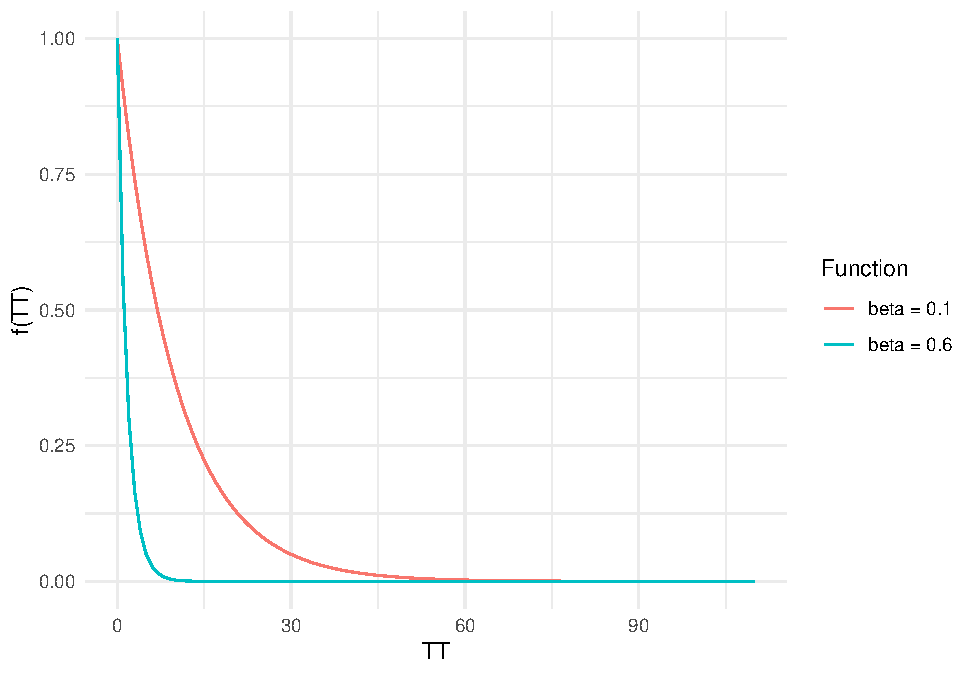
\includegraphics[width=1\linewidth]{Spatial-Availability-Refreshed_files/figure-latex/comparison-impedance-functions-synthetic-example-1} \caption{\label{fig:impedance-functions-comparison}Comparison of two negative exponential impedance functions used in the synthetic example. The x-axis represents the travel time (in mins) and the y-axis represents the impedance function at each travel time.}\label{fig:comparison-impedance-functions-synthetic-example}
\end{figure}

As expected, Hansen-type accessibility drops quite dramatically after
this \(\beta\) modification: the friction of distance is so high that
few opportunities are within reach. In contrast, Shen-type accessibility
converges to the jobs:population ratio (i.e., origin \(A\) is
\(\frac{100,000}{50,000} = 2\)). This is explained by the way the
impedance function excludes the population in droves, thus reducing the
competition for jobs: as seen in Table \ref{tab:synthetic-example}, the
effective opportunity-seeking population from \(A\) is only about equal
to 6.17; likewise, the number of jobs at 1 weighted by the impedance is
only 12.341. In other words, competition is low because jobs are
expensive to reach, but those willing to reach jobs enjoy relatively
high accessibility (in the limit, the jobs/population ratio). On the
other hand, the accessibility is effectively zero for those in the
population prevented by the impedance from reaching any jobs.

In what follows, we propose an alternative derivation of {[}26{]}
accessibility with competition that explicitly clarifies the
opportunities allocated to the \emph{effective opportunity-seeking
population} within its formulation. Hence, the results are not only more
interpretable, but also extend the potential of accessibility analysis.

\hypertarget{introducing-spatial-availability-a-singly-constrained-measure-of-accessibility}{%
\section{Introducing spatial availability: a singly-constrained measure
of
accessibility}\label{introducing-spatial-availability-a-singly-constrained-measure-of-accessibility}}

In brief, we define the \emph{spatial availability} at \(i\) (\(V_{i}\))
as the proportion of all opportunities \(O\) that are allocated to \(i\)
from all destinations \(j\): \[
V_i = \sum_{j=1}^NO_jF^t_{ij}
\]

\noindent where:

\begin{itemize}
\tightlist
\item
  \(F^t_{ij}\) is a balancing factor that depends on the population and
  cost of movement in the system.
\item
  \(O_j\) is the number of opportunities at \(j\).
\item
  \(V_i\) is the number of spatially available opportunities from the
  perspective of \(i\).
\end{itemize}

The general form of spatial availability is also as a sum, and the
fundamental difference with Hansen- and Shen-type accessibility is that
opportunities are allocated proportionally. Balancing factor
\(F^t_{ij}\) consists of two components: a population-based balancing
factor \(F^p_{i}\) and an impedance-based balancing factor \(F^c_{ij}\)
which, respectively, allocate opportunities to \(i\) in proportion to
the size of the population of the different competing centers (the mass
effect of the gravity model) and the cost of reaching opportunities (the
impedance effect). In the next two subsections, we explain the intuition
behind the method before defining it in full.

\hypertarget{proportional-allocation-by-population}{%
\subsection{Proportional allocation by
population}\label{proportional-allocation-by-population}}

According to the gravity modelling framework, the potential for
interaction depends on the mass (i.e., the population) and the friction
of distance (i.e., the impedance function). We begin by describing the
proposed proportional allocation mechanism based on demand by
population. Recall, the total population in the example is 210,000. The
proportion of the population by population center is as follows: \[
\begin{array}{l}
F^p_A = \frac{50,000}{210,000}\\
\\
F^p_B = \frac{150,000}{210,000}\\
\\
F^p_C = \frac{10,000}{210,000}\\
\end{array}
\]

Jobs are allocated proportionally from each employment center to each
population center depending on their population sizes as per the
balancing factors \(F^p_i\). In this way, employment center 1 allocates
\(100,000\cdot \frac{50,000}{210,000}= 23,809.52\) jobs to \(A\);
\(100,000\cdot \frac{150,000}{210,000}= 71,428.57\) jobs to \(B\); and
\(100,000\cdot \frac{10,000}{210,000}= 7,142.857\) jobs to \(C\). Notice
how this mechanism ensures that the total number of jobs at employment
center 1 is preserved at 100,000.

We can verify that the number of jobs allocated is consistent with the
total number of jobs in the system: \[
\begin{array}{l}
\text{Employment center 1 to population centers A, B, and C: }\\
100,000 \cdot \frac{50,000}{210,000} + 100,000 \cdot \frac{150,000}{210,000} + 100,000 \cdot \frac{10,000}{210,000} = 100,000\\
\\
\text{Employment center 2 to population centers A, B, and C: }\\
100,000 \cdot \frac{50,000}{210,000} + 100,000 \cdot \frac{150,000}{210,000} + 100,000 \cdot \frac{10,000}{210,000} = 100,000\\
\\
\text{Employment center 3 to population centers A, B, and C: }\\
10,000 \cdot \frac{50,000}{210,000} + 10,000 \cdot \frac{150,000}{210,000} + 10,000 \cdot \frac{10,000}{210,000} = 10,000\\
\end{array}
\]

In the general case where there are \(N\) population centers in the
region, we define the following population-based balancing factors in
Equation (\ref{eq:population-balancing-factor}):

\begin{equation}
\label{eq:population-balancing-factor}
F^p_{i} = \frac{P_{i}^\alpha}{\sum_{i=1}^N P_{i}^\alpha}
\end{equation}

Balancing factor \(F^p_{i}\) corresponds to the proportion of the
population in origin \(i\) relative to the population in the region. On
the right hand side of the equation, the numerator \(P_{i}^\alpha\) is
the population at origin \(i\). The summation in the denominator is over
\(i=1,\cdots,N\), and adds up to the total population of the region.
Notice that we incorporate an empirical parameter \(\alpha\). The role
of \(\alpha\) is to modulate the effect of demand by population. When
\(\alpha <1\), opportunities are allocated more rapidly to smaller
centers relative to larger ones; \(\alpha>1\) achieves the opposite
effect.

Balancing factor \(F^p_{i}\) can now be used to proportionally allocate
a share of available jobs at \(j\) to origin \(i\). The number of jobs
available to \(i\) from \(j\) balanced by population shares is defined
as follows: \[
V^p_{ij} = O_j\frac{F^p_{i}}{\sum_{i=1}^N F^p_{i}}
\]

In the general case where there are \(J\) employment centers, the total
number of jobs available from all destinations to \(i\) is simply the
sum of \(V^p_{ij}\) over \(j=1,\cdots, J\): \[
V^p_{i} = \sum_{j=1}^J O_j\frac{F^p_{i}}{\sum_{i=1}^N F^p_{i}}
\]

Since the factor \(F^p_{i}\), when summed over \(i=1,\cdots,N\) always
equals to 1 (i.e., \(\sum_{i=1}^{N} F^p_{i} = 1\)), the sum of all
spatially available jobs equals \(O\), the total number of opportunities
in the region: \[
\begin{array}{l}
\sum_{i=1}^N V^p_i =\sum_{i=1}^N\sum_{j=1}^JO_j\frac{F^p_{i}}{\sum_{i=1}^N F^p_{i}}\\
=\sum_{i=1}^N \frac{F^p_{i}}{\sum_{i=1}^N F^p_{i}}\cdot\sum_{j=1}^JO_j\\
=\sum_{j=1}^J O_j = O
\end{array}
\] The terms \(F^p_{i}\) act here as the balancing factors of the
gravity model when a single constraint is imposed {[}i.e., to ensure
that the sums of columns are equal to the number of opportunities per
destination, see 53 and 183-184{]}. As a result, the sum of spatial
availability for all population centers equals the total number of
opportunities.

The discussion so far concerns only the mass effect (i.e., population
size) of the gravity model. In addition, the potential for interaction
is thought to decrease with increasing cost, so next we define similar
balancing factors but based on the impedance.

\hypertarget{proportional-allocation-by-cost}{%
\subsection{Proportional allocation by
cost}\label{proportional-allocation-by-cost}}

Clearly, using only balancing factors \(F^p_{i}\) to calculate spatial
availability \(V^p_i\) does not account for the cost of reaching
employment centers. Consider instead a set of balancing factors
\(F^c_{ij}\) that account for the friction of distance for our example.
Recall that the impedance function \(f(c_{ij})\) equals
\(\exp(-\beta\cdot c_{ij})\) where \(\beta = 0.1\) and travel time
\(c_{ij}\) is either 15, 30 or 60 minutes. For instance, the
impedance-based balancing factors \(F^c_{ij}\) would be the following
for employment center 1 (employment center 2 and 3 have their own
balancing factor values for each origin \(i\) as will be discussed
later): \[
\begin{array}{l}
F^c_{A1} = \frac{0.223130}{0.223130 + 0.049787 + 0.000045} = 0.8174398\\
F^c_{B1} = \frac{0.049787}{0.223130 + 0.049787 + 0.000045} = 0.1823954\\
F^c_{C1} = \frac{0.000045}{0.223130 + 0.049787 + 0.000045} = 0.0001648581\\
\end{array}
\]

Balancing factors \(F^c_{ij}\) use the impedance function to
proportionally allocate more jobs to closer population centers, that is,
to those with populations \emph{more willing to reach the jobs}. Indeed,
the factors \(F^c_{ij}\) can be thought of as the proportion of the
population at \(i\) willing to travel to destination \(j\), conditional
on the travel behavior as given by the impedance function. For instance,
\({81.74398}\%\) of jobs from employment center 1 are allocated to
population center \(A\) based on impedance.

So as follows from our example, of the 100,000 jobs at employment center
1 the number of jobs allocated to population center \(A\) is
\(100,000\times 0.8174398 = 81,743.98\) jobs; the number allocated to
population center \(B\) is \(100,000\times 0.1823954 = 18,239.54\) jobs;
and the number allocated to population center \(C\) is
\(100,000\times 0.0001648581 = 16.48581\) jobs. We see once more that
the total number of jobs at the employment center is preserved at
100,000. In this example, the proportional allocation mechanism assigns
the largest share of jobs to population center \(A\), which is the
closest to employment center 1, and the smallest to the more distant
population center \(C\).

In the general case where there are \(N\) population centers and \(J\)
employment centers in the region, we define the following
impedance-based balancing factors:

\begin{equation}
\label{eq:impedance-balancing-factor}
F^c_{ij} = \frac{f(c_{ij})}{\sum_{i=1}^N f(c_{ij})}
\end{equation}

The total number of jobs available to \(i\) from \(j\) according to
impedance is defined as follows: \[
V^c_{ij} = O_j\frac{F^c_{ij}}{\sum_{i=1}^N F^c_{ij}}
\]

The total number of jobs available to \(i\) from all destinations is: \[
V^c_{i} = \sum_{j=1}^J O_j\frac{F^c_{ij}}{\sum_{i=1}^N F^c_{ij}}
\]

Like the population-based allocation factors, \(F^c_{i}\) summed over
\(i=1,\cdots,N\) always equals to 1 (i.e.,
\(\sum_{i=1}^{N} F^c_{ij} = 1\)). As before, the sum of all spatially
available jobs equals \(O\), the total number of opportunities in the
region: \[
\begin{array}{l}
\sum_{i=1}^N V^c_i =\sum_{i=1}^N\sum_{j=1}^JO_j\frac{F^c_{ij}}{\sum_{i=1}^N F^c_{ij}}\\
=\sum_{i=1}^N \frac{F^c_{ij}}{\sum_{i=1}^N F^c_{ij}}\cdot\sum_{j=1}^JO_j\\
=\sum_{j=1}^J O_j = O
\end{array}
\]

We are now ready to more formally define spatial availability with due
consideration to both population and travel cost effects.

\hypertarget{assembling-mass-and-impedance-effects}{%
\subsection{Assembling mass and impedance
effects}\label{assembling-mass-and-impedance-effects}}

Population and the cost of travel are both part of the gravity modelling
framework. Since the balancing factors defined in the preceding sections
are proportions (alternatively, can be understood as probabilities),
they can be combined multiplicatively to obtain their joint effect. This
multiplicative relationship can alternatively be understood as the joint
probability of allocating opportunities and is captured by Equation
(\ref{eq:balancing-factors}), where \(F^p_{i}\) is the population-based
balancing factor that grants a larger share of the existing
opportunities to larger centers and \(F^c_{ij}\) is the impedance-based
balancing factor that grants a larger share of the existing
opportunities to closer centers. This is in line with the tradition of
gravity modeling.

\begin{equation}
\label{eq:balancing-factors}
F^t_{ij} = \frac{F^p_{i} \cdot F^c_{ij}}{\sum_{i=1}^N F^p_{i} \cdot F^c_{ij}}
\end{equation}

\noindent with \(F^p_{i}\) and \(F^c_{ij}\) as defined in Equations
(\ref{eq:population-balancing-factor}) and
(\ref{eq:impedance-balancing-factor}) respectively. The combined
balancing factor \(F^t_{ij}\) is used to proportionally allocate jobs
from \(j\) to \(i\). Hence, spatial availability is given by Equation
(\ref{eq:spatial-availability}).

\begin{equation}
\label{eq:spatial-availability}
V_{i} = \sum_{j=1}^J O_j\ F^t_{ij}
\end{equation}

The terms in Equation \ref{eq:spatial-availability} are as follows:

\begin{itemize}
\tightlist
\item
  \(F^t_{ij}\) is a balancing factor as defined in Equation
  (\ref{eq:balancing-factors}).
\item
  \(i\) is a set of origin locations in the region \(i = 1,\cdots, N\).
\item
  \(j\) is a set of destination locations in the region
  \(j = 1,\cdots,J\).
\item
  \(O_j\) is the number of opportunities at location \(j\).
\item
  \(V_{i}\) is the spatial availability at \(i\).
\end{itemize}

Notice that, unlike \(S_i\) in Hansen-type accessibility (Equation
(\ref{eq:conventional-accessibility})), the population enters the
calculation of \(V_{i}\) through \(F^p_i\). Returning to the example in
Figure \ref{fig:plot-toy-example}, Table \ref{tab:synthetic-example}
also contains the information needed to calculate \(V_i\), with
\(\beta\) set again to 0.1. Column \textbf{V\_ij} are the jobs available
to each origin from each employment center. In this column \(V_{A1}=\)
59,901 is the number of jobs available at \(A\) from employment center
1. Column \textbf{V\_i} (i.e., \(\sum_{j=1}^JV_{ij}\)) gives the total
number of jobs available to origin \(i\). We can verify that the total
number of jobs available is consistent with the total number of jobs in
the region (with some small rounding error): \[
\sum_{i=1}^N V_i = 66,833 + 133,203 + 9,963 \approx 210,000 
\]

Compare the calculated values of \(V_i\) to column \textbf{S\_i}
(Hansen-type accessibility) in Table \ref{tab:synthetic-example}. The
spatial availability values are more intuitive. Recall that population
centers \(A\) and \(B\) had identical Hansen-type accessibility to
employment opportunities. According to \(V_i\), population center \(A\)
has greater job availability due to: 1) its close proximity to
employment center 1; combined with 2) less competition (i.e., a majority
of the population have to travel longer distances to reach employment
center 1). Job availability is lower for population center \(B\) due to
much higher competition (150,000 people can reach 100,000 jobs at equal
cost). And center \(C\) has almost as many jobs available as it has
population.

As discussed above, Hansen-type accessibility is not designed to
preserve the number of jobs in the region. Shen-type accessibility ends
up preserving the number of jobs in the region but the definitions of
variables are internally obscured; the only way it preserves the number
of jobs is if the effect of the impedance function is ignored when
expanding the values of jobs per capita to obtain the total number of
opportunities. The proportional allocation procedure described above, in
contrast, consistently returns a number of jobs available that matches
the total number of jobs in the region.

Since the jobs spatially available are consistent with the jobs in the
region, it is possible to define a measure of spatial availability per
capita as presented in Equation (\ref{eq:SA-per-capita}):

\begin{equation}
\label{eq:SA-per-capita}
v_i = \frac{V_i}{P_i}
\end{equation}

And, since the jobs are preserved, it is possible to use the regional
jobs per capita (\(\frac{\sum_{j=1}^J O_j}{\sum_{i=1}^N P_i}\)) as a
benchmark to compare the spatial availability of jobs per capita at each
origin.

In the example, since the population is equal to the number of jobs, the
regional value of jobs per capita is \(1.0\). To complete the
illustrative example, the spatial availability of jobs per capita by
origin is:

\begin{equation}
\label{eq:SA-per-capita-2populations}
\begin{array}{l}
v_{1} = \frac{V_1}{P_1} =  \frac{66,833.47}{50,000} = 1.337\\
v_{2} =  \frac{V_{2}}{P_2} =  \frac{133,203.4}{150,000} = 0.888\\
v_{3} =  \frac{V_{3}}{P_3} =  \frac{9,963.171}{10,000} = 0.996\\
\end{array}
\end{equation}

We can see that population center \(A\) has fewer jobs per capita than
the regional benchmark, center \(B\) has more, and center \(C\) is at
parity. Remarkably, the spatial availability per capita matches the
values of \(a_i\) in Table \ref{tab:synthetic-example}. Appendix A has a
proof of the mathematical equivalence between the two measures. It is
interesting to notice how {[}28{]}, {[}26{]}, as well as this paper, all
reach identical expressions starting from different assumptions; this
effect is known as \emph{equifinality} {[}see 53,and 54{]}. This result
means that Shen-type accessibility and 2SFCA can be re-conceptualized as
singly-constrained accessibility measures.

\hypertarget{why-does-proportional-allocation-matter}{%
\subsection{Why does proportional allocation
matter?}\label{why-does-proportional-allocation-matter}}

We have shown that Shen-type accessibility and spatial availability
produce equifinal results when accessibility per-capita is computed. At
this point it is reasonable to ask whether the distinction between these
two measures is of any importance.

Conceptually, we would argue that the confounded populations in
Shen-type accessibility leads to internal inconsistency in the
calculation of total opportunities in {[}26{]}: this points to a deeper
issue that is only evident when we consider the intermediate values of
the method. To illustrate, Table \ref{tab:synthetic-example} shows
results of \(a_i\) that are reasonable (and they match exactly the
spatial availability per capita). But when we dig deeper, these results
mask potentially misleading values for the jobs allocated and the number
of jobs taken. For instance, a region with a high jobs:population ratio
but a prohibitive transportation network that results in a high cost of
travel may yield a high \(a_i\) value. This value, however, can conceal
a low \emph{effective opportunity-seeking population} and proportionally
low number of allocated jobs while additionally obscuring the number of
population which does \emph{not} take jobs and the jobs \emph{not}
taken.

In addition, the intermediate accessibility values of \(a_i\) (Shen-type
measure) may also lead to impact estimates that are deceptive {[}see
55{]}. For example, the estimated region-wide cost of travel considering
the jobs allocated by \(a_i\) in Table \ref{tab:synthetic-example}
(i.e., \(Jobs*f(TT)\)) is as follows:

\[
\begin{array}{l}
22,313\times 15 \text{ min} + 4,979\times 30 \text{ min} + 0.454\times 100 \text{ min}\\
4,979\times 30 \text{ min} + 22,313\times 15 \text{ min} + 0.454\times 100 \text{ min}\\
4.54\times 100 \text{ min} + 4.54\times 100 \text{ min} + 2,231\times 15 \text{ min} = 1,002,594\text{ min}
\end{array}
\]

In contrast, the estimated region-wide cost of travel according to
\(V_i\) in Table \ref{tab:synthetic-example} is as follows: \[
\begin{array}{l}
59,901\times 15 \text{ min} + 6,923\times 30 \text{ min} + 10\times 100 \text{ min}\\
40,097\times 30 \text{ min} + 93,076\times 15 \text{ min} + 30\times 100 \text{ min}\\
2.4\times 100 \text{ min} + 1.3\times 100 \text{ min} + 9,959\times 15 \text{ min} = 3,859,054\text{ min}
\end{array}
\]

Often referred to as `the supply of jobs' (or simply Hansen-style
accessibility) in the Shen-type measure: \(Jobs*f(TT)\) cannot be used
to understand the region-wide cost of travel. Recall how we define
\(Pop*f(TT)\) as the \emph{effective opportunity-seeking population}
(\(P^*_{ij}\)), \(Jobs*f(TT)\) similarly represents the \emph{effective
\textbf{opportunities allocated}} and sums to approximately 56,824 out
of a total of 210,000 jobs. Like \(Pop*f(TT)\), the \emph{effective
opportunities allocated} to each origin is only a reflection of the
impedance function and not the \emph{actual} number of opportunities
allocated to each origin. Therefore, the resulting
\(1,002,594\text{ min}\) is not a meaningful measure of the cost of
travel in the system.

However, since spatial availability allocates the \emph{actual} number
of opportunities to each origin; the 3,859,054\text{ min} can be used to
quantify the system-wide impacts of competitive accessibility in this
region. We know spatial availability's output is the number of
opportunities at each \(i\) since the combined balancing factors
allocate a proportional amount of the total opportunities to each \(i\)
such that the number of opportunities allocated to each \(i\) sum to
equal the total opportunities in the region.

\hypertarget{empirical-example-of-toronto}{%
\section{Empirical example of
Toronto}\label{empirical-example-of-toronto}}

In this section we illustrate the application of spatial availability
through an empirical example. For this, we use full-time employment
flows from the Greater Golden Horseshoe (GGH) area in Ontario, Canada.
Contained with the GGH is the Greater Toronto and Hamilton (GTHA) which
forms the most populous metropolitan regions in Canada and the core
urban agglomeration in the GGH.

The GTHA contains the city of Toronto, the most populous city in Canada.
The city of Toronto is the focus of this empirical example, it will be
used to demonstrate the application of the proposed spatial availability
measure along with how it compares to Hansen- and Shen-type measures. We
begin this section by explaining the data and then detailing the
calculated comparisons.

\hypertarget{ggh-data}{%
\subsection{GGH Data}\label{ggh-data}}

We obtained full-time employment flows from the 2016 Transportation
Tomorrow Survey (TTS). This survey collects representative urban travel
information from 20 municipalities contained within the GGH area in the
southern part of Ontario, Canada (see Figure
\ref{fig:TTS-16-survey-area}) {[}56{]} every five years. The data set
includes origin to destination flows associated with full-time
employment trips; the number of jobs (n=3,081,885) and workers
(n=3,446,957) (i.e., the number of originating trips and destination
trips) at each origin and destination are represented at the level of
Traffic Analysis Zones (TAZ) (n=3,764). TAZ are a unit of spatial
analysis which are defined as part of the TTS, however, TAZ are commonly
used to ascribe production and attraction of trips in the context of
transportation planning modelling. In the GGH data set, the TAZ contain
on average 916 workers and jobs 819 with more detailed descriptive
statistics discussed later. The TTS data is based on a representative
sample of between 3\% to 5\% of households in the GGH and is weighted to
reflect the population covering the study area as a whole {[}56{]}.

To generate the travel cost for the full-time employment trips, travel
times between origins and destinations (i.e., centroids of the TAZ) are
calculated for car travel using the \texttt{R} package \{r5r\} {[}57{]}
with a street network retrieved from OpenStreetMap. It is also assumed
that intra-TAZ trips are equal to 0.1 minutes. For inter-TAZ trips, a 3
hr travel time threshold was selected as it captures 99\% of
population-employment pairs (see the travel times summarized in Figure
\ref{fig:TTS-16-survey-area}). This method does not account for traffic
congestion or modal split, which can be estimated through other means
{[}e.g., 58,59{]}. For simplicity, we carry on with the assumption that
all trips are taken by car in uncongested travel conditions. All data
and data preparation steps are documented and can be freely explored in
the companion open data product
\href{https://soukhova.github.io/TTS2016R/}{\{TTS2016R\}}.

\begin{figure}

{\centering 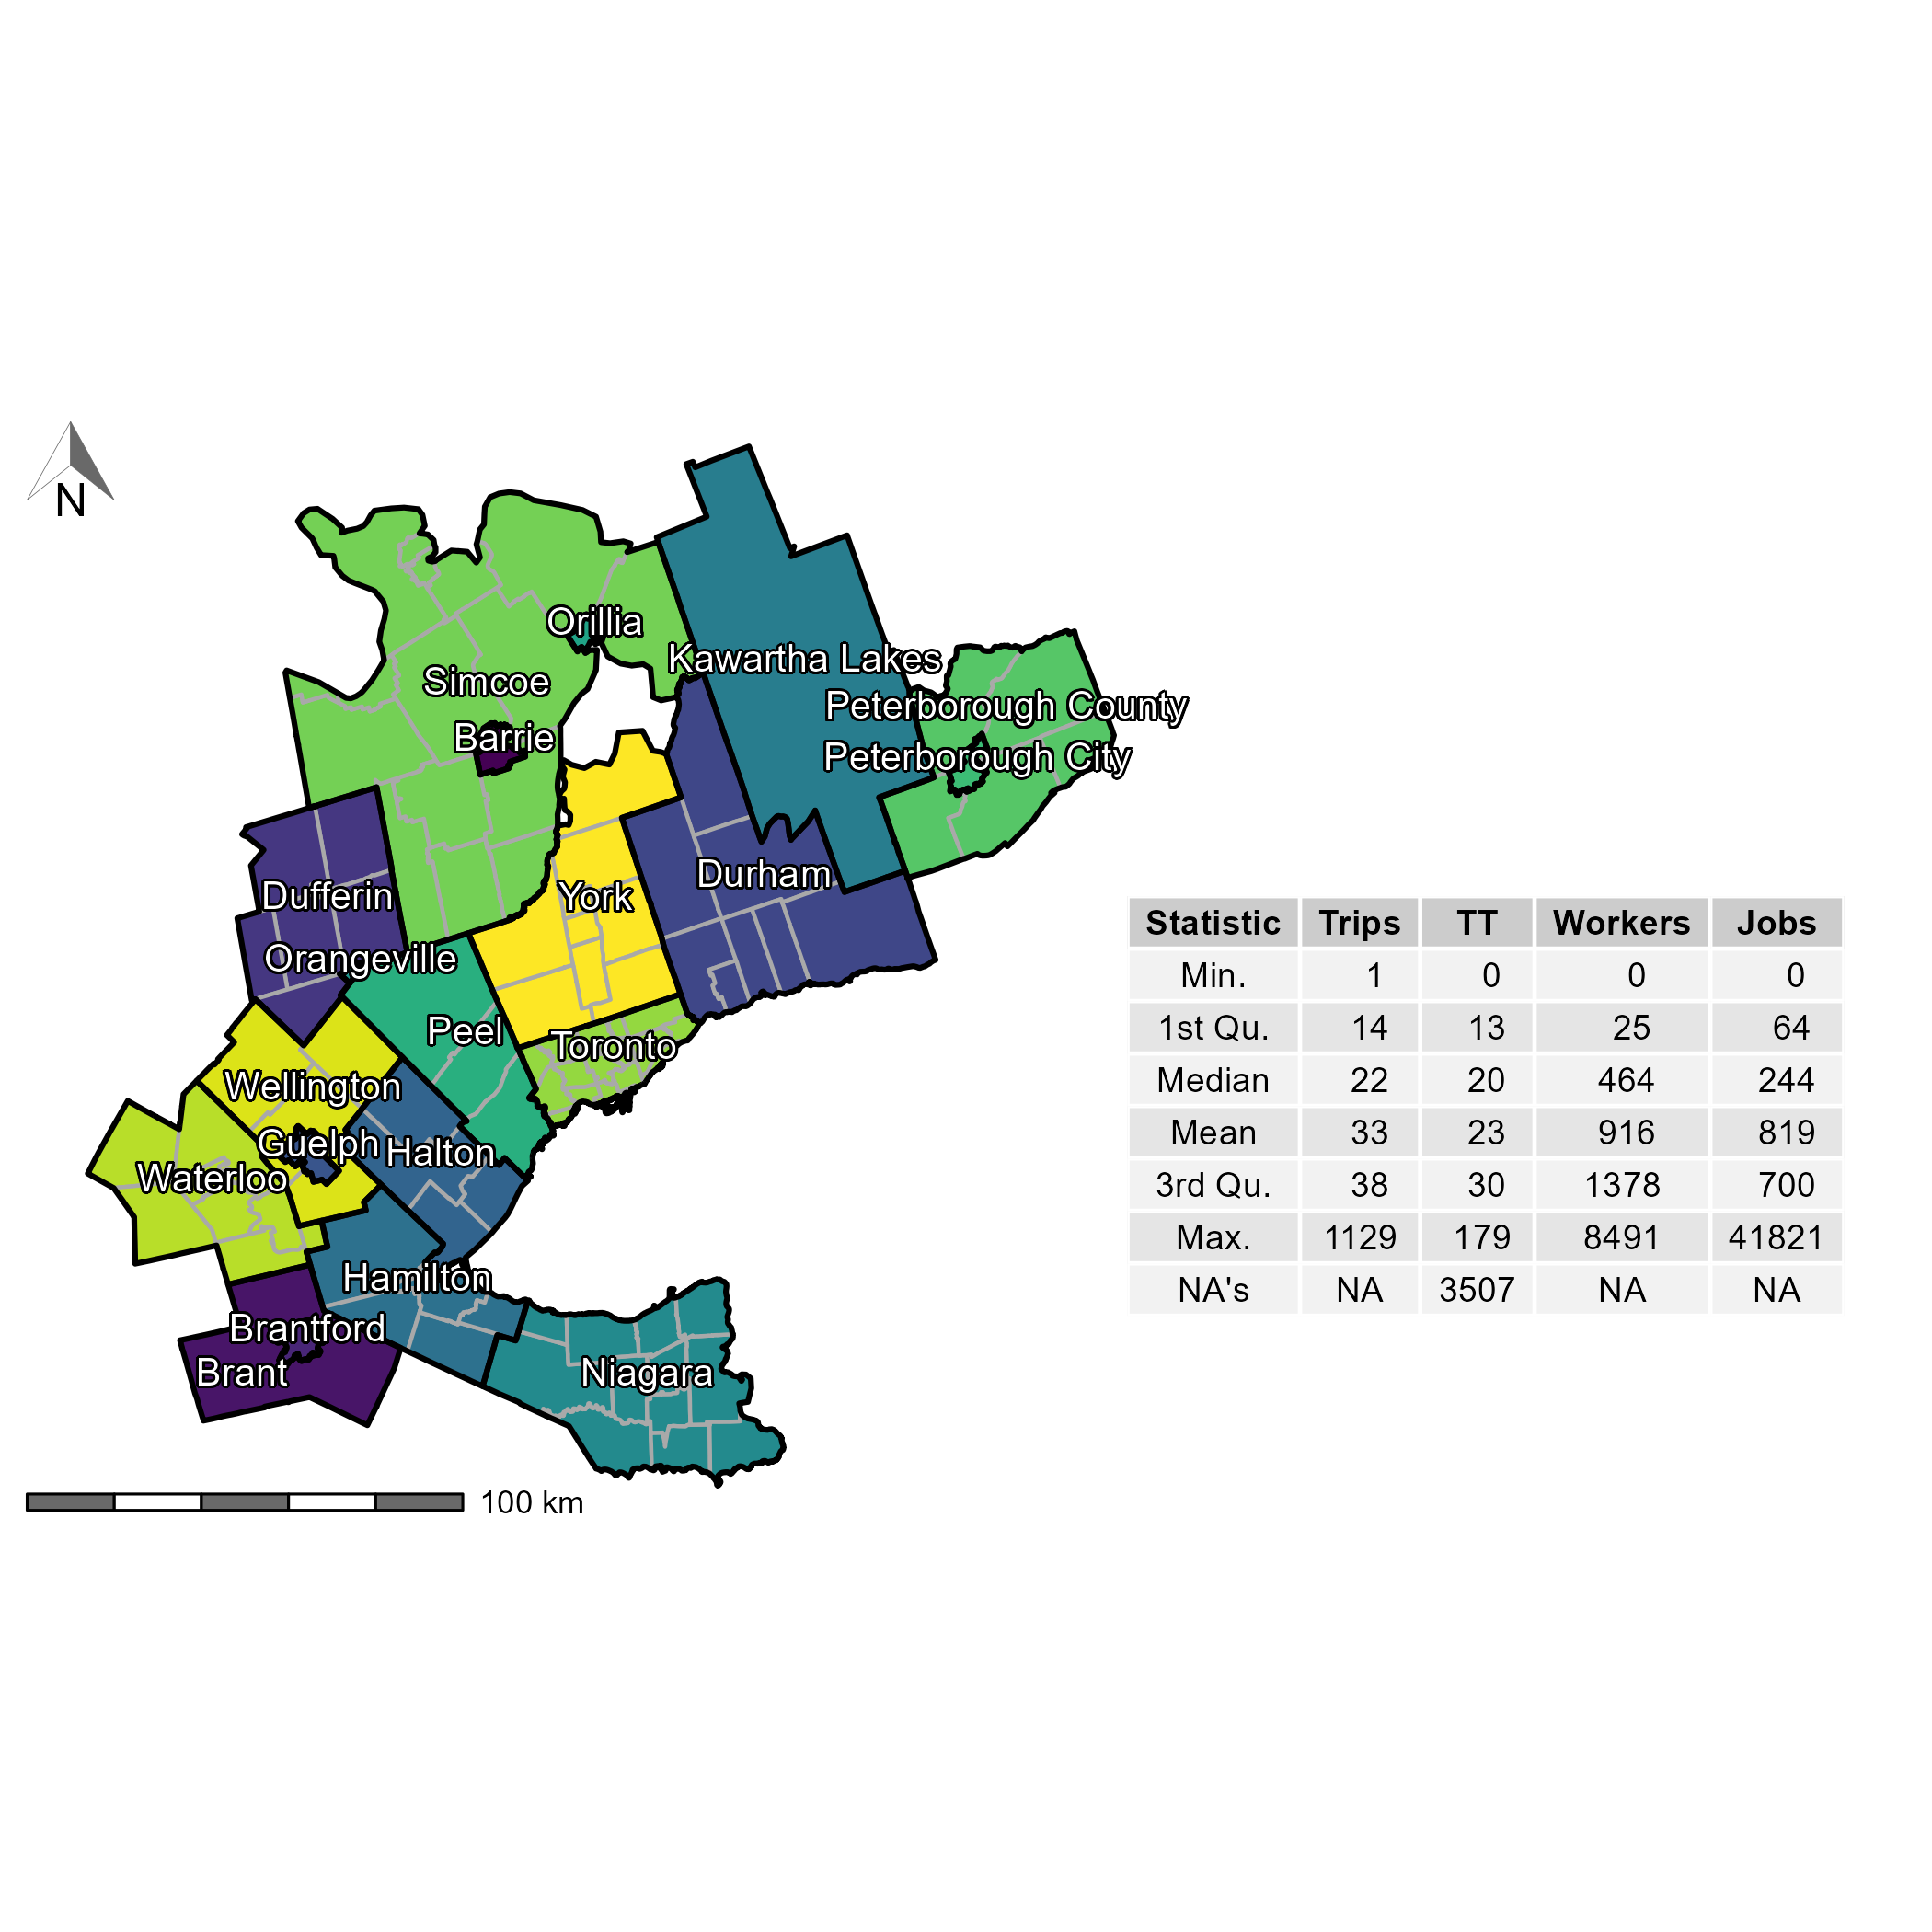
\includegraphics[width=1\linewidth]{images/TTS16-survey-area} 

}

\caption{\label{fig:TTS-16-survey-area}TTS 2016 study area (GGH, Ontario, Canada) along with the descriptive statistics of the trips, calculated origin-destination car travel time (TT), workers per TAZ, and jobs per TAZ. Contains 20 regions (black boundaries) and sub-regions (dark gray boundaries).}\label{fig:TTS-16-survey-area}
\end{figure}

\hypertarget{spatial-employment-characteristics-in-toronto}{%
\subsection{Spatial employment characteristics in
Toronto}\label{spatial-employment-characteristics-in-toronto}}

\begin{figure}
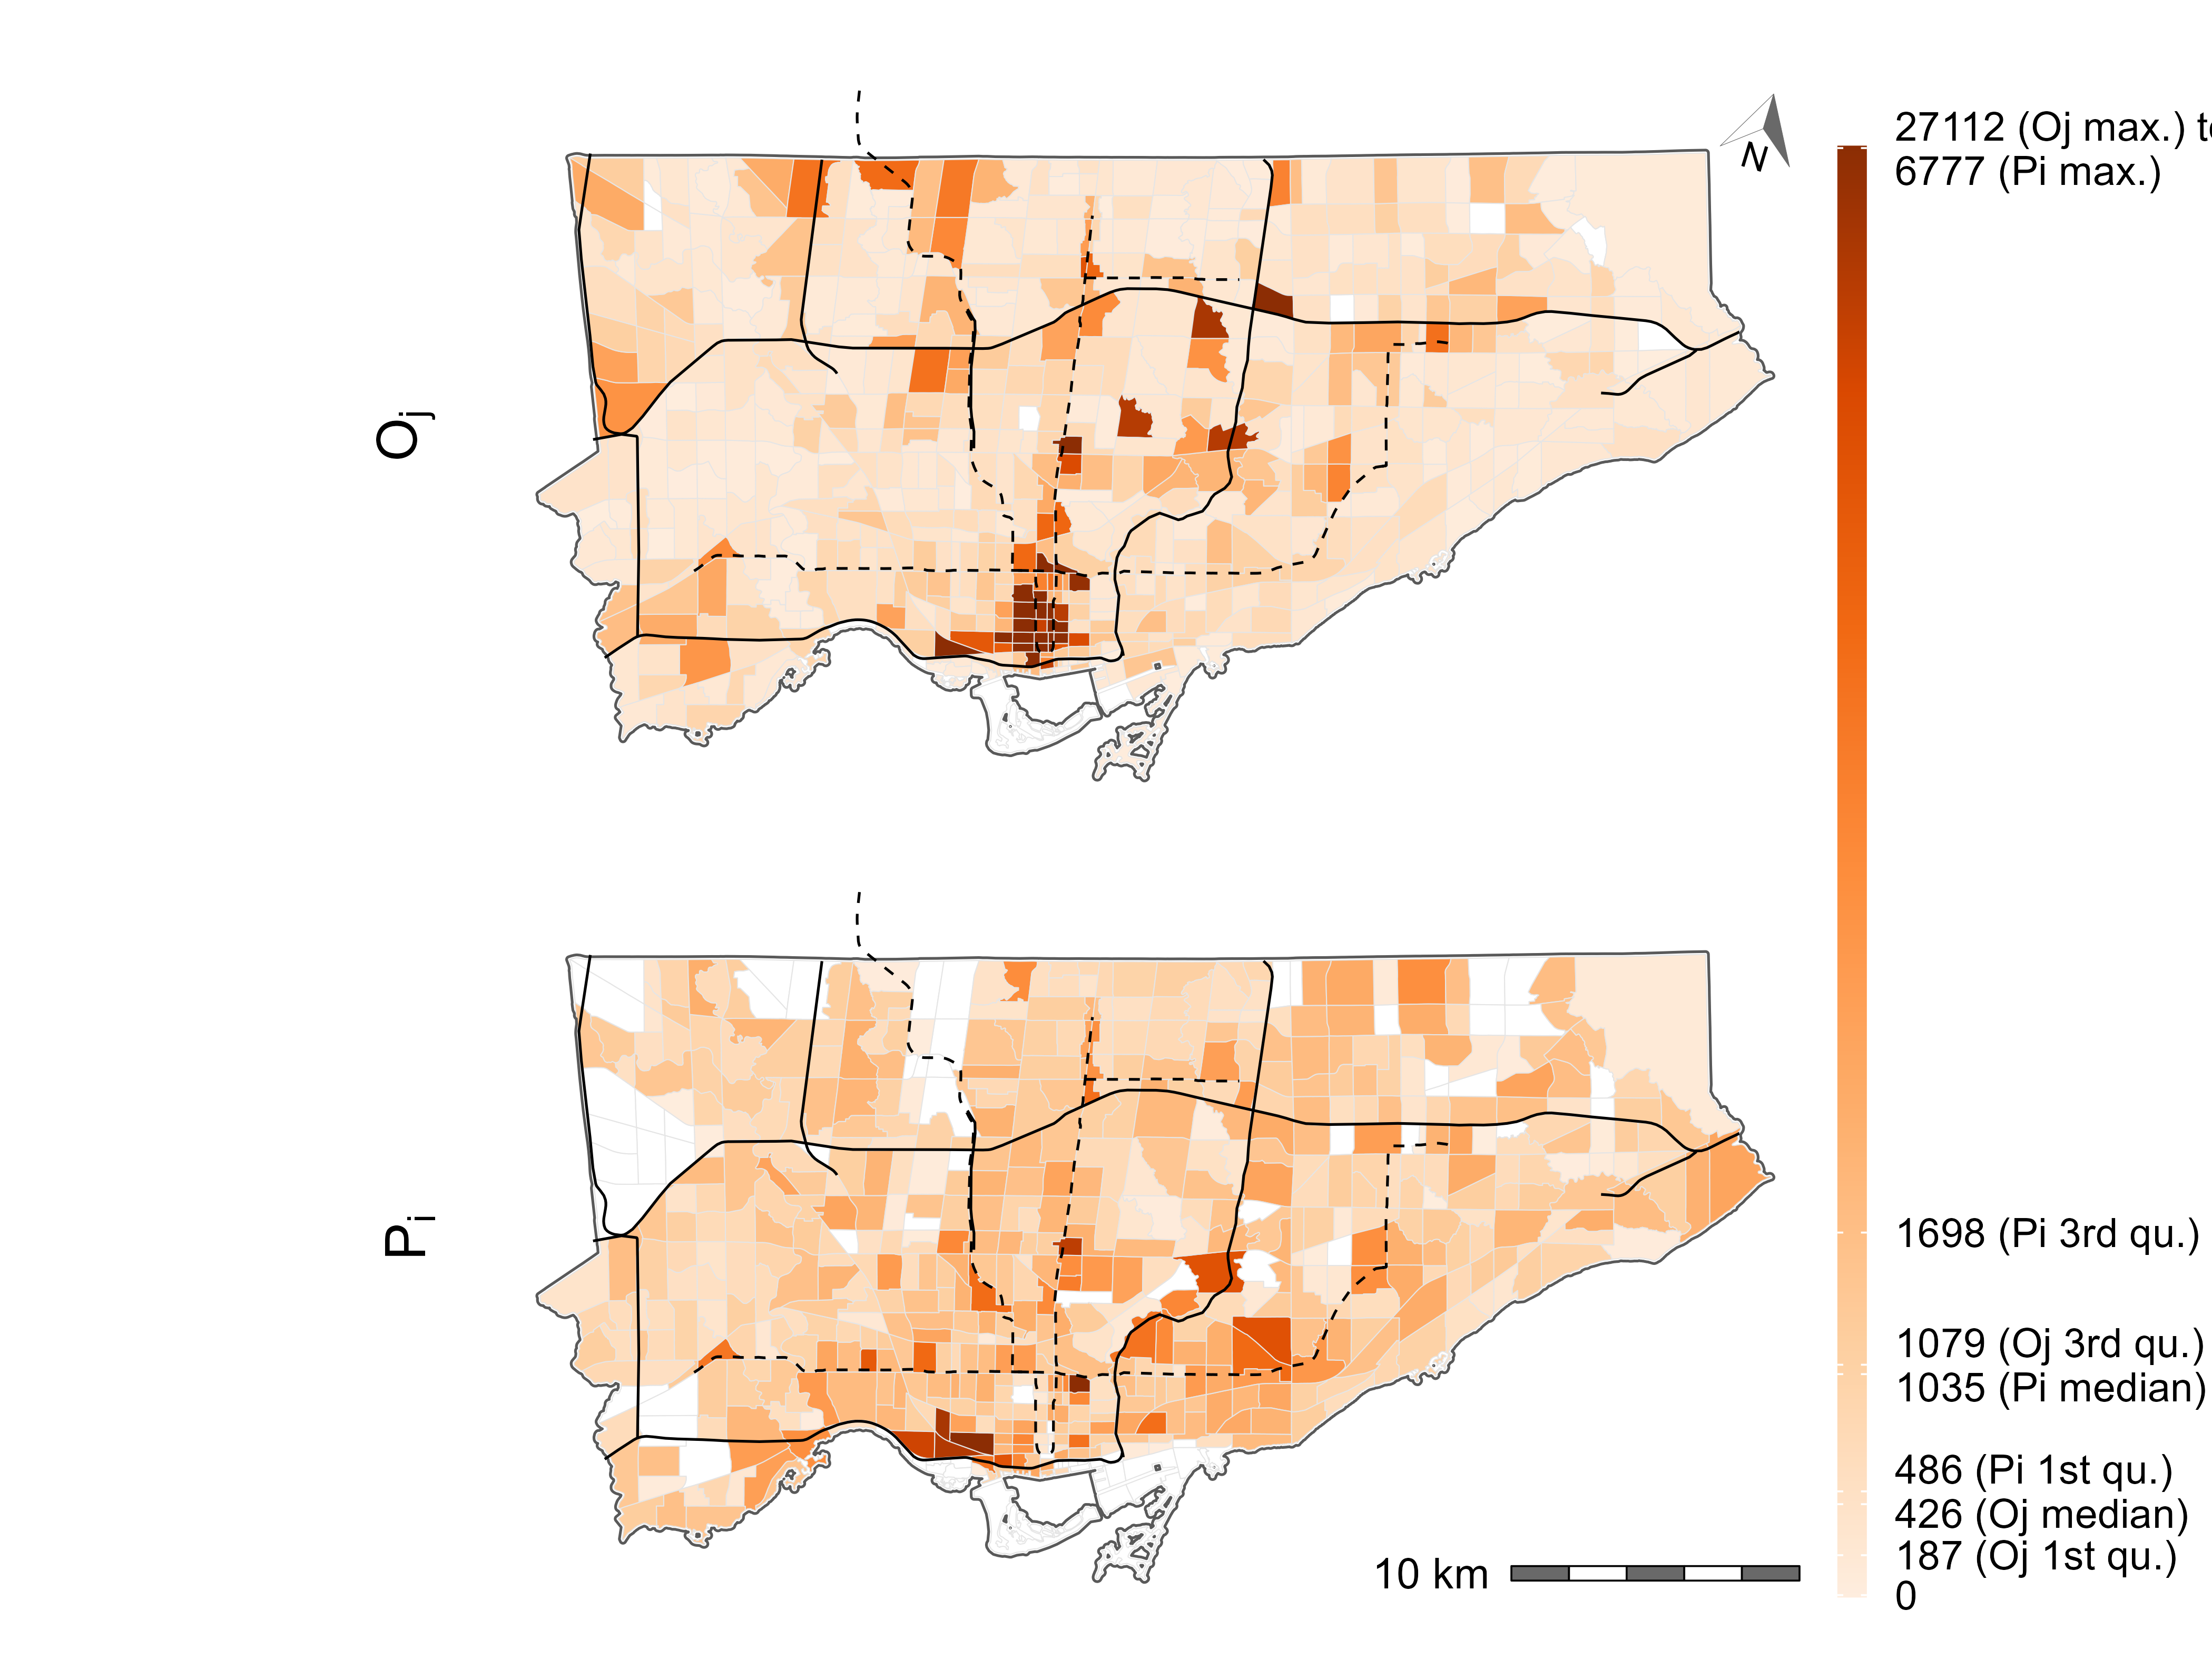
\includegraphics[width=1\linewidth]{images/spatial-dist-jobs-pop-Toronto-plot} \caption{\label{fig:s-dist-Toronto-plot}  Spatial distribution of full-time jobs (top) and full-time working population (bottom) at each TAZ for Toronto as provided by the 2016 TTS. Black lines represent expressways and black dashed lines represent subway lines. All white TAZ have no worker population or jobs.}\label{fig:spatial-dist-Toronto-plot}
\end{figure}

\begin{figure}
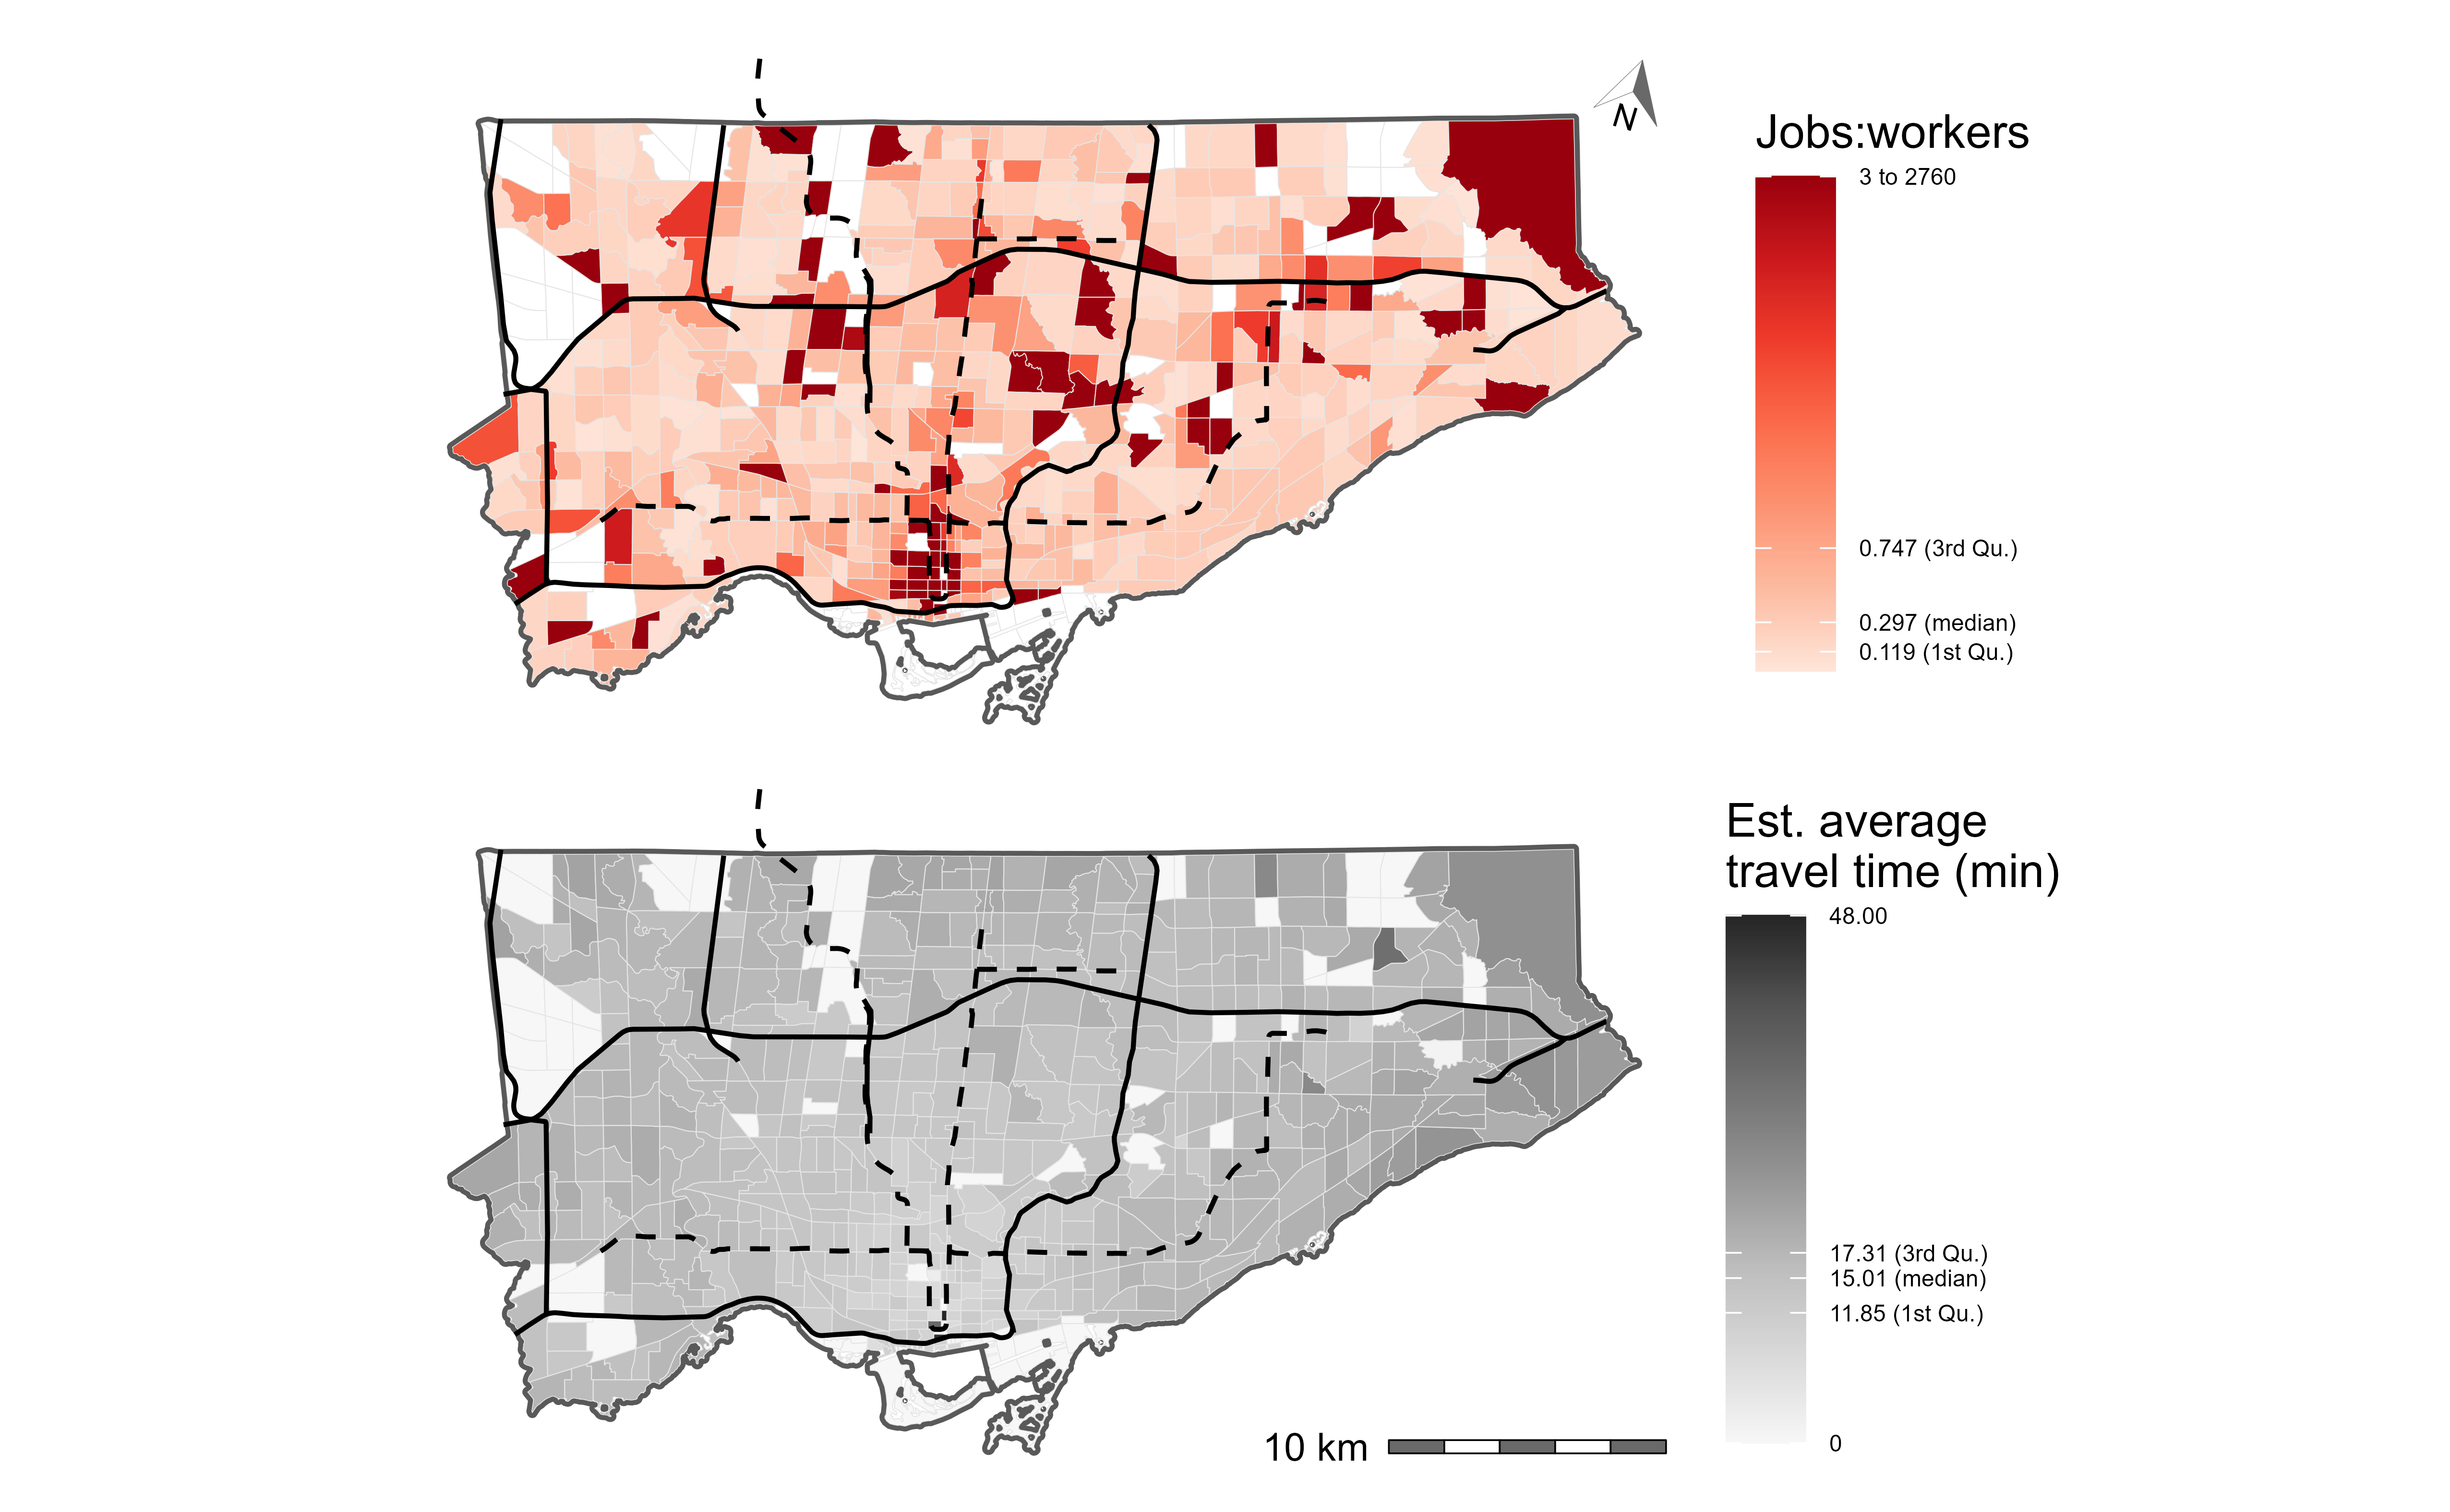
\includegraphics[width=1\linewidth]{images/spatial-dist-jobs-pop-Toronto-plot2} \caption{\label{fig:s-dist-Toronto-plot2}  Spatial distribution of full-time working population to jobs ratio (top) and car travel time to jobs estimated using R5R (bottom) for the city of Toronto as provided by the 2016 TTS. Black lines represent expressways and black dashed lines represent subway lines. White TAZ represent a TAZ with no workers thus no travel time for the top plot, for the bottom plot they represent no travel time TAZ and TAZ with only 1 travel time.}\label{fig:spatial-dist-Toronto-plot2}
\end{figure}

As mentioned, the focus of this empirical example is on the city of
Toronto. It is the largest city in the GGH and represents a significant
subset of workers and jobs in the GGH; 22\% of workers in the GGH live
in Toronto and 25\% of jobs that these workers take are located within
Toronto. The spatial distribution of jobs and workers is shown in Figure
\ref{fig:s-dist-Toronto-plot}. It can be seen that a large cluster of
jobs can be found in the central southern part of Toronto (the downtown
core). Spatial trends in the distribution of workers is more even
relative to the distribution of jobs.

Next, the spatial distribution of the estimated car travel time (green)
and the associated standard deviation (grey) is visualized in Figure
\ref{fig:s-dist-Toronto-plot2}. It can be seen that the car travel time
is lower within the downtown core and, unexpectedly higher as the TAZ is
further from the downtown core. These travel time estimations are to be
expected, as these car travel time are calculated using an uncongested
OpenStreetMaps road network from the centroid of origin TAZ to
destination TAZ. Since within Toronto trips are only considered, trips
which originate from the center of Toronto, an area with high job
density, relatively closer proximity to all other Toronto TAZ, and high
road connectivity, travel times are lower than outside in an areas
further from the downtown core. In terms of the variability of the
travel times, the center TAZ of Toronto have lower variability than TAZ
closer to the borders of Toronto. Trends from both plots indicate that
trips originating from within the center of Toronto are shorter and more
similar in length than traips originating from closer to the border of
Toronto.

Nonetheless, the point of these visualizations is to demonstrate the
spatial distribution of worker and job data in the city of Toronto to
contextualize spatial availability and Shen- and Hansen- type measures.

\hypertarget{calibration-of-an-impedance-function-for-toronto}{%
\subsection{Calibration of an impedance function for
Toronto}\label{calibration-of-an-impedance-function-for-toronto}}

In the synthetic example introduced before, we used a negative
exponential function with the parameter reported by {[}26{]}. For the
empirical Toronto data set, we calibrate an impedance function on the
trip length distribution (TLD) of commute trips. Briefly, a TLD
represents the proportion of trips that are taken at a specific travel
cost (e.g., travel time); this distribution is commonly used to derive
impedance functions in accessibility research {[}60--62{]}.

As mentioned, the calculations are undertaken for the city of Toronto
using only the employed population in the city and jobs taken by
residents of Toronto. Specifically, edge trips are not included such as
trips originating in Toronto but finishing outside of Toronto and trips
originating outside of Toronto but finishing in Toronto. The empirical
and theoretical TLD for this Toronto data set are represented in the
top-left panel of Figure \ref{fig:TLD-norm-plot}. Maximum likelihood
estimation and the Nelder-Mead method for direct optimization available
within the \{fitdistrplus\} package {[}63{]} were used. Based on
goodness-of-fit criteria and diagnostics the normal distribution was
selected (see Figure \ref{fig:TLD-norm-plot}).

\begin{figure}

{\centering 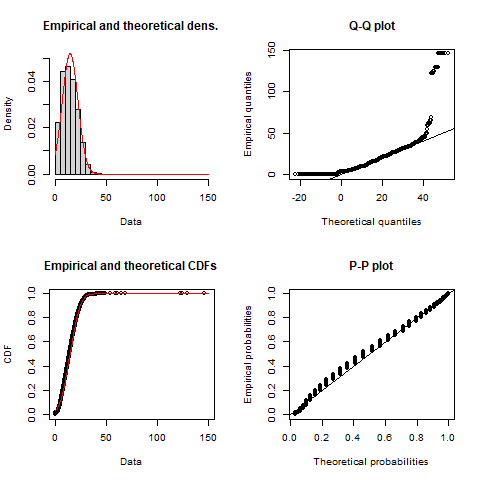
\includegraphics[width=1\linewidth]{images/impedance_function} 

}

\caption{\label{fig:TLD-norm-plot}Car trip length distribution and calibrated normal distribution impedance function (red line) with associated Q-Q and P-P plots. Based on the estimated car travel times for full-time employment and workers in Toronto from the TTS 2016.}\label{fig:TLD-norm-plot}
\end{figure}

The normal distribution is defined in Equation (\ref{norm-dist}), where
we see that it depends on a mean parameter \(\mu\) and a standard
deviation parameter \(\sigma\). The estimated values of these parameters
are \(\mu=\) 14.169 and \(\sigma =\) 7.369.

\begin{equation}
\label{norm-dist}
\begin{array}{l} 
f(x) = \frac{1}{\sigma \sqrt{2\pi}}e^{-\frac{1}{2}(\frac{x-\mu}{\sigma})^2}\\
\end{array}
\end{equation}

\[
\frac{1}{\sigma \sqrt{2\pi}}e^{\frac{1}{2}(\frac{x-\mu}{\sigma})^2}
\]

\hypertarget{accessibility-and-spatial-availability-of-jobs-in-toronto}{%
\subsection{Accessibility and spatial availability of jobs in
Toronto}\label{accessibility-and-spatial-availability-of-jobs-in-toronto}}

\hypertarget{absolute-opportunity-values}{%
\subsubsection{Absolute opportunity
values}\label{absolute-opportunity-values}}

\begin{figure}
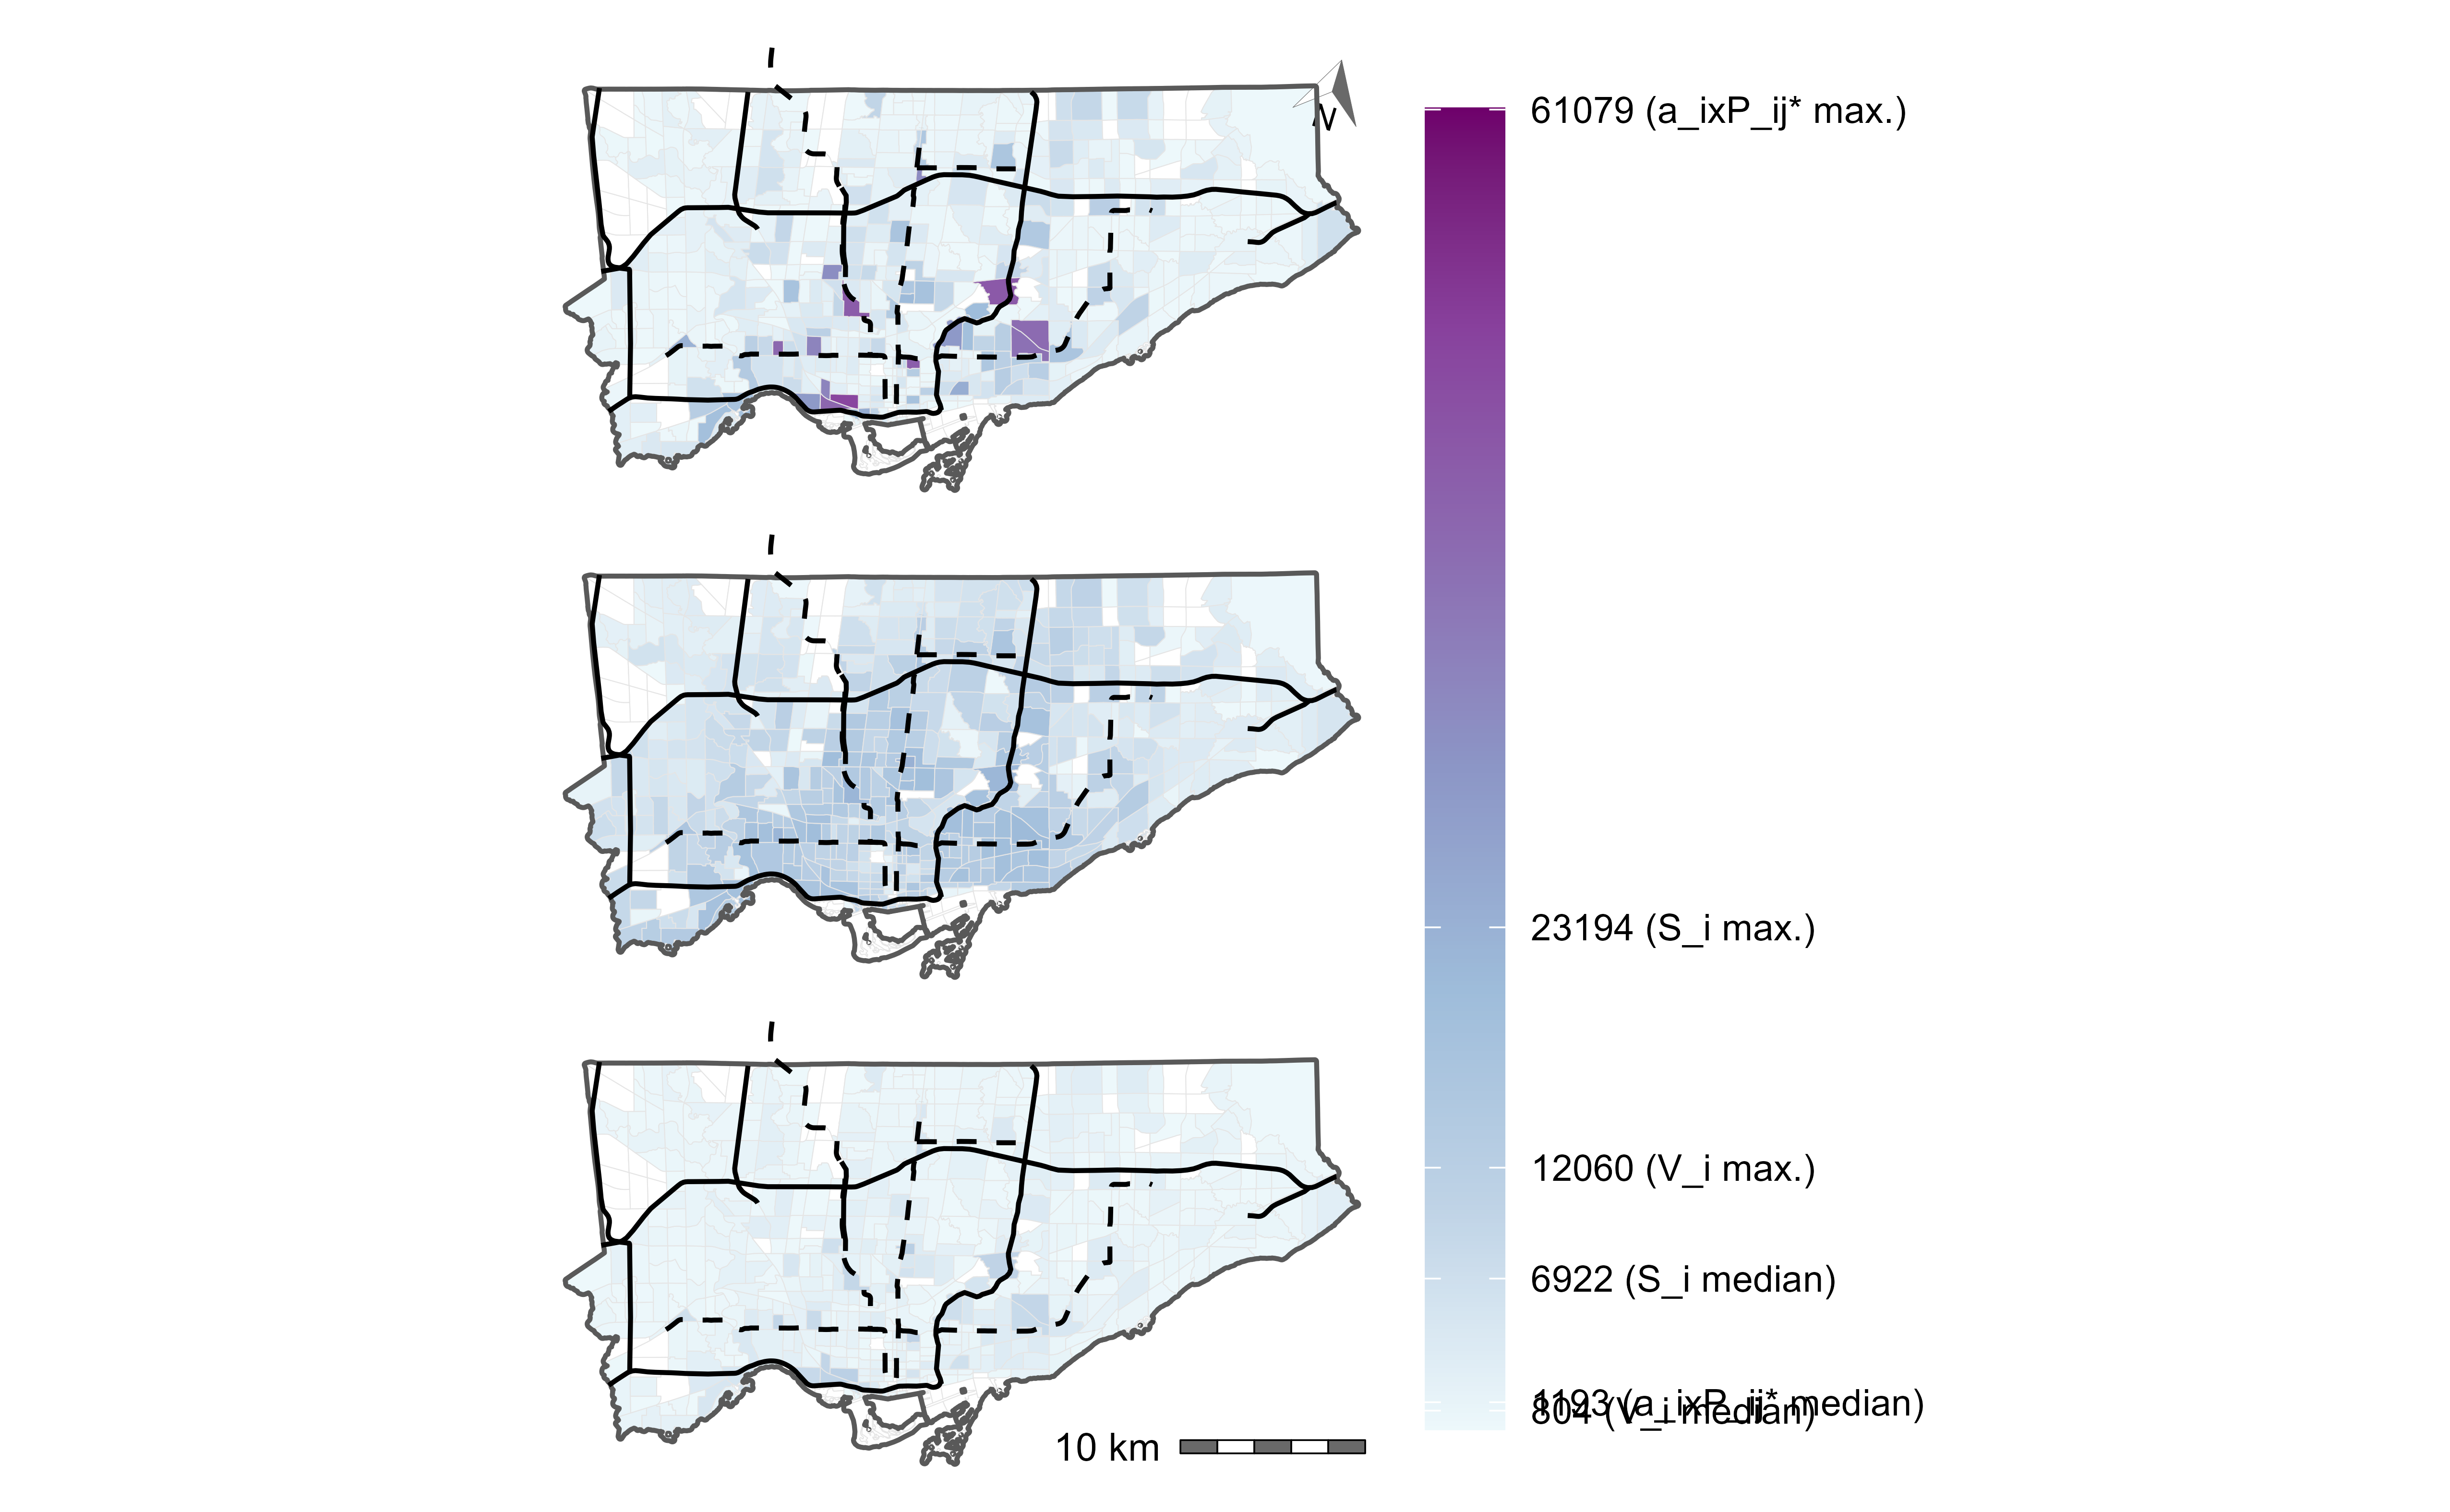
\includegraphics[width=1\linewidth]{images/access-job-Toronto-plot} \caption{\label{fig:absolute-accessibility-plot}Estimated accessibility to jobs (\# of jobs) in Toronto according to Shen-type measure times effective opportunity-seeking population (top), Hansen-type measure (middle), and spatial availability (bottom). Black lines represent expressways and black dashed lines represent subway lines. All white TAZ have no worker population or jobs, i.e., with null accessibility values. Legend scale is square root transformed to effectively visualize the spread range.}\label{fig:absolute-accessibility-plot}
\end{figure}

Figure \ref{fig:absolute-accessibility-plot} contains the number of jobs
accessible using Shen-type accessibility, Hansen-type accessibility, and
the number of jobs \emph{available} using the spatial availability
measure. The values from all these measures are represented on the same
axis as they are comparable as they measure the absolute value of
\emph{jobs} accessible to the workers in the origin. In the top plot,
the Shen-type accessibility is multiplied by the \emph{effective
opportunity-seeking population} to yield a value that corresponds to
absolute number of accessible jobs (considering competition) according
to Shen's definition. In the middle plot, the Hansen-type accessibility
is an unconstrained case of accessibility in which all jobs which are
in-reach of each origin (according to the impedance function); each
value corresponds to the number of jobs which can be reach at each
origin assuming no competition. Lastly, in the bottom plot, the spatial
availability measure is a constrained case of accessibility which yields
the number of jobs, at each origin, considering competition from the
population in nearby origin and the relative travel cost (according to
the impedance function).

What is notable about the bottom plot is that the proportional
allocation mechanism of spatial availability ensures that the job
availability value for each origin all sums to the city-wide total of
769,231 jobs (i.e., the number of destination flows from Toronto origins
to Toronto destinations). The number of accessible jobs at each origin
can therefore be interpreted as the number of \emph{available} jobs to
each origin based on the relative travel behaviour and density of
competition for jobs (i.e., worker population). A proportion of each of
the 769,231 jobs in Toronto are only allocated once to each origin. In
terms fo the middle plot, the city-wide total for Hansen-type
accessibility is 4,366,743 jobs, which as a value is meaningless since
the measure is unconstrained; it represents the sum of opportunities
that have been counted anywhere from 1 to many times depending on the
impedance function. As previously discussed, unconstrained counting of
the same opportunity by all origins is not an issue if the opportunity
itself is non-exclusive, but since one job can only be given to one
worker (especially since the worker and job data is derived from
origin-destination flows), it is inappropriate to use unconstrained
measures to capture employment characteristics. Comparing the middle and
bottom plots, it is evident that the unconstrained counting of
opportunities (Hansen-style) results in absolute values that are higher
throughout the city, particularly in TAZ that are in proximity to high
job density (recall Figure \ref{fig:s-dist-Toronto-plot}). These same
trends are not present in the spatial availability bottom plot, as the
absolute value is lower than Hansen-style accessibility as the proximity
to high job density and competition from worker density is
proportionally metered; the resulting values are thus lower than the
middle plot and reflect the spatial distribution trends of both the
workers and job density (recall Figure \ref{fig:s-dist-Toronto-plot}).

Lastly, the top plot that visualizes the \emph{absolute} Shen-type
measure (as understood by Shen's definition of \(P_i\) being equal to
\(P_{ij}^*\) sums to the city-wide value of 2,117,774 by multiplying
\(a_i\) by the \emph{effective opportunity-seeking population}
\(P_{ij}^*\) (i.e., the denominator of the rate ). This plot thus
demonstrates how confounding \(P_i\) with \(P_{ij}^*\) yields an
\emph{incorrect} number of competitively accessible jobs: it is
evidently incorrect because the sum of \(a_iP_{ij}^*\) greatly exceeds
the city-wide total of workers (i.e., 2,117,774 \textgreater{} 769,231).
To the authors' knowledge, literature has not attempted to convert
Shen-type accessibility to the absolute value of accessible jobs in the
way demonstrated in the top plot: we suspect this is the case because of
the ambiguous definition that conflates \(P_{ij}^*\) with \(P_i\). If
\(a_i\) is multiplied by \(P_i\), it yields the same value as \(V_i\),
but since the definition of Shen-type measure is equivocal doing so is
not clear since the denominator of \(a_i\) (which is a rate) is
\emph{not} \(P_i\). The resulting plot, spatially, is similar to spatial
availability (bottom plot) but certain TAZ have exceptionally high
values in an inconsistent way. This is because \(a_i\) uses the
impedance function values for both access to jobs (numerator) and the
competition from neighboring workers (denominator \(P_{ij}^*\)) to
adjust their impact: using \(P_{ij}^*\) does not \emph{consistently}
isolate the absolute value of accessible jobs. However, if \(a_i\) is
multiplied by \(P_i\) it yields the same values at \(V_i\) (bottom plot)
(the proof for mathematically equivalency is in Appendix A). As also
mentioned earlier, the formulation of the denominator and numerator of
\(a_i\) is ambigious so to presume that multiplying it by \(P_i\) would
disintangle the rate and yield the absolute value of accessible
\emph{and available} (i.e., considering competition) jobs is unclear.

\hypertarget{internal-values}{%
\subsubsection{Internal values}\label{internal-values}}

\begin{figure}
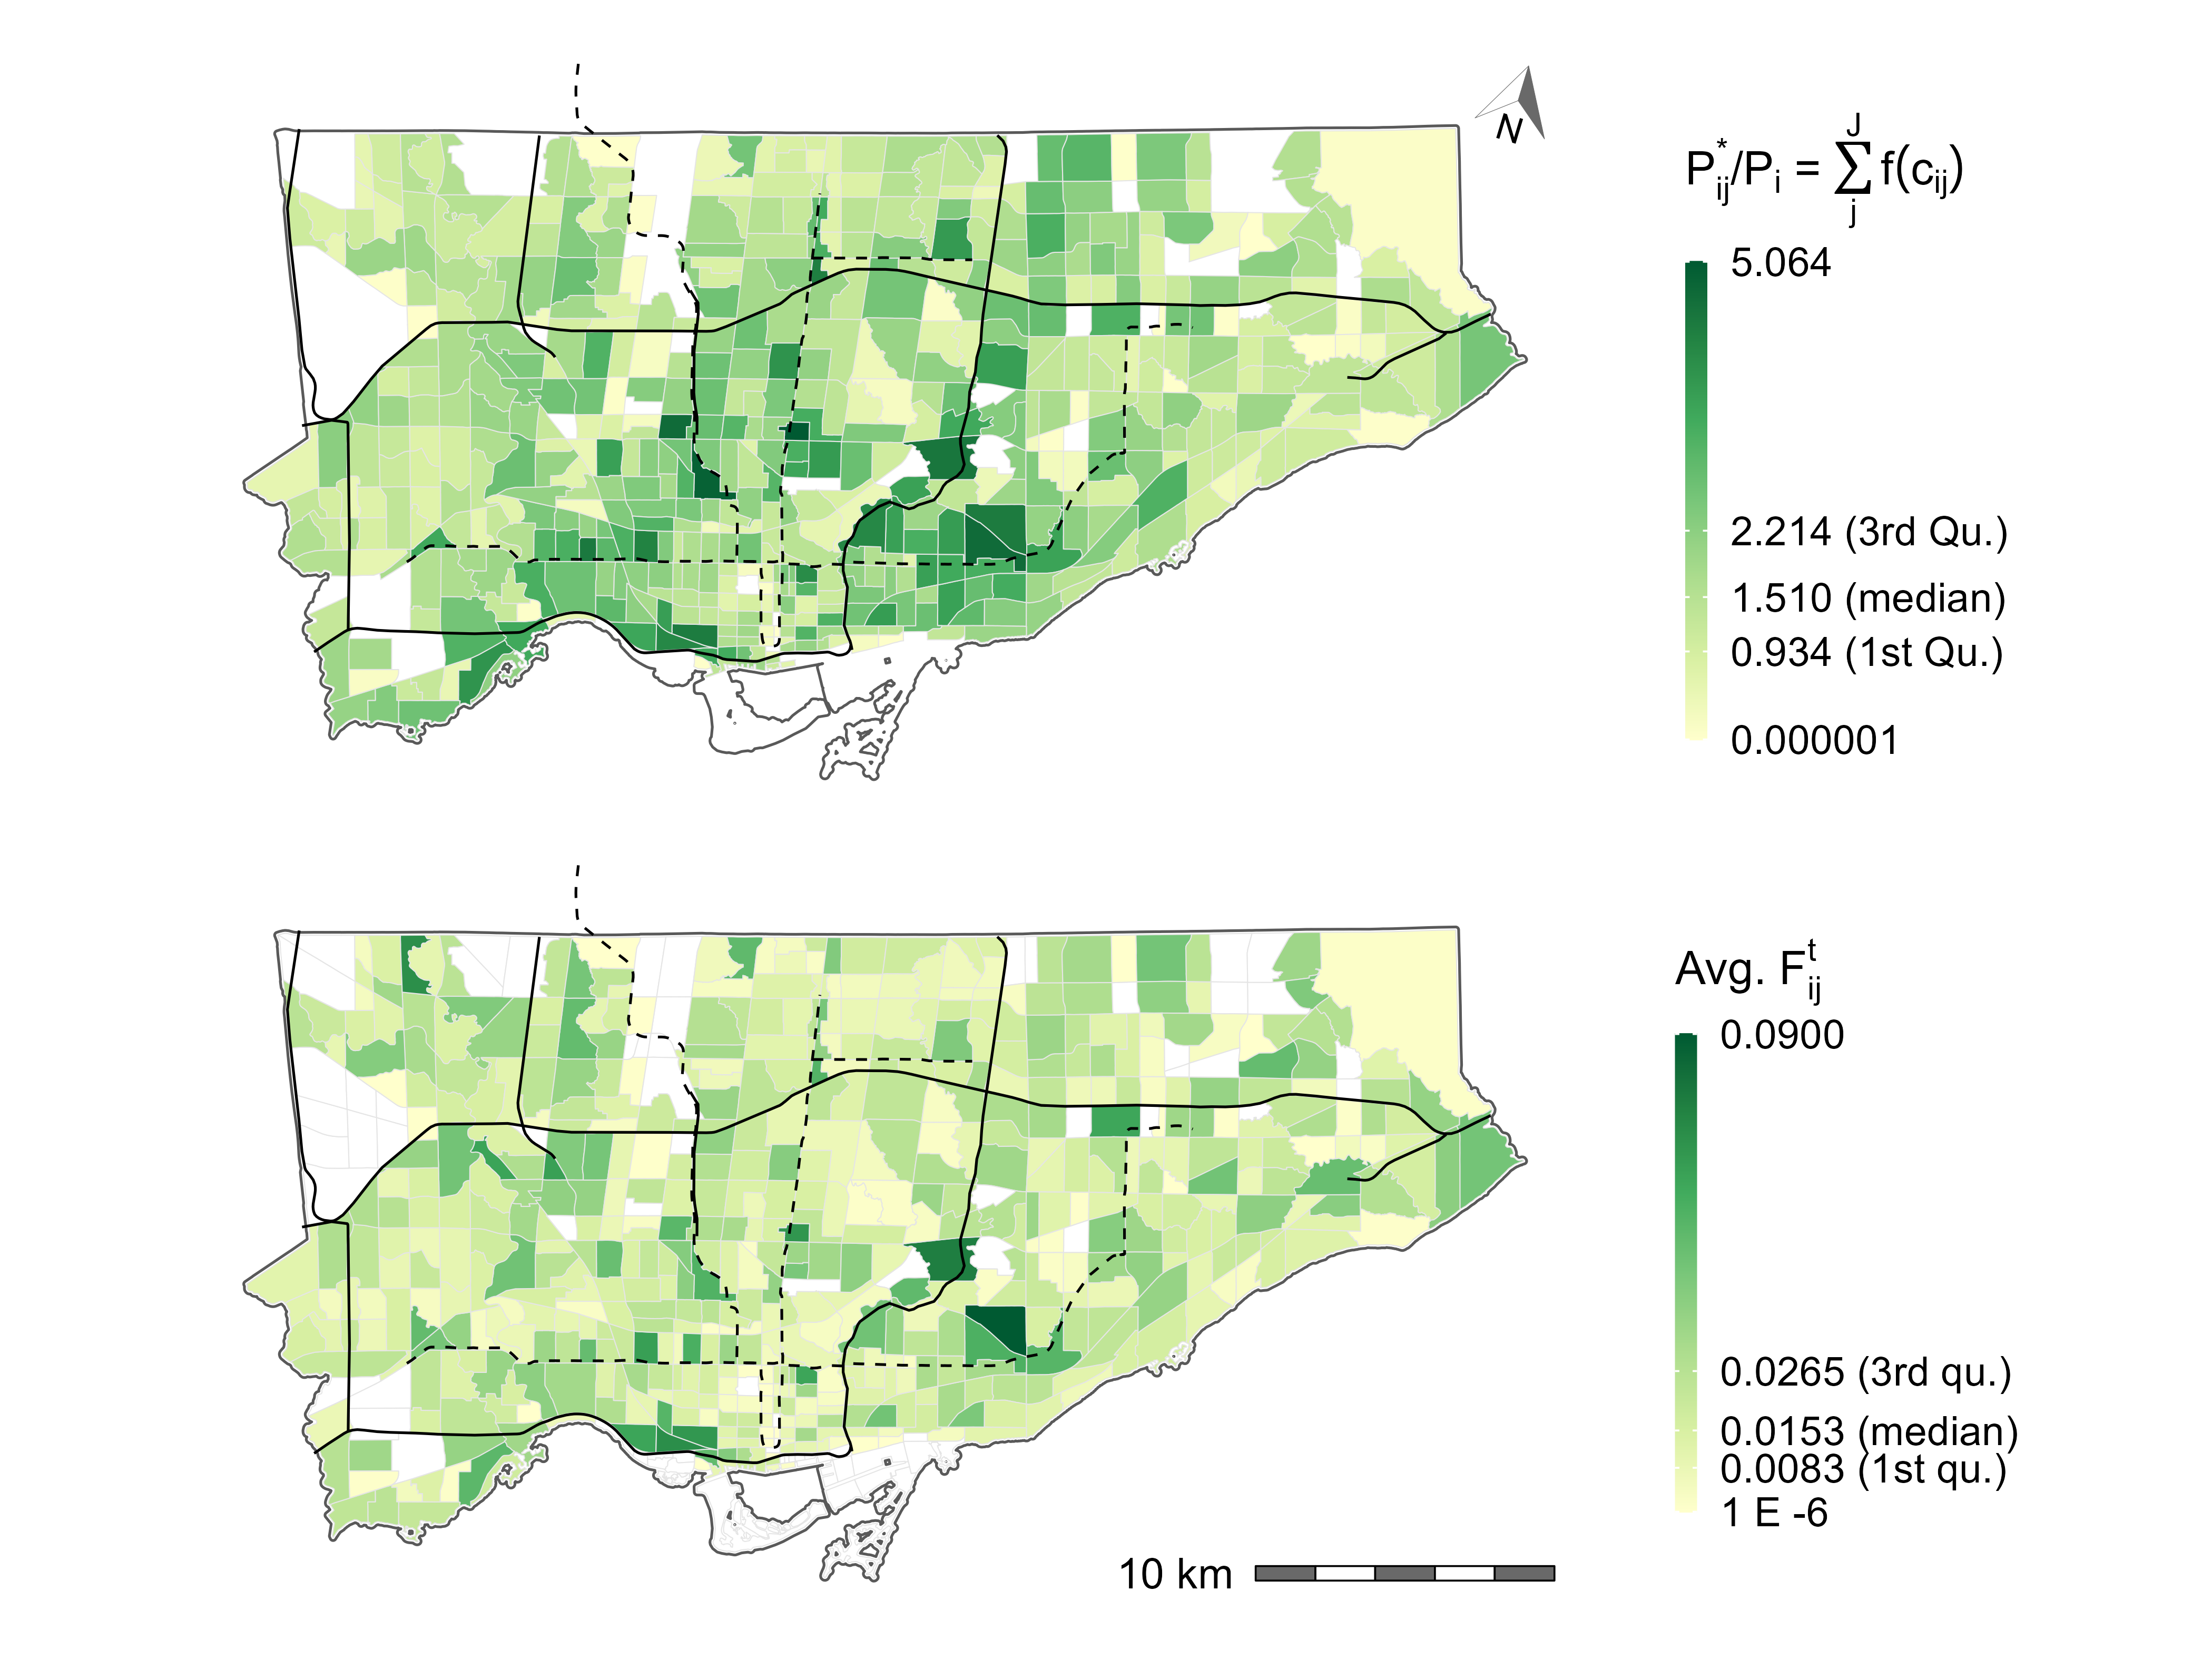
\includegraphics[width=1\linewidth]{images/internal-values-plot} \caption{\label{fig:internal-values-plot}  The ratio of the effective opportunity seeking population to the population (top) and the average spatial availability's balancing factor (Equation (9)) (bottom) for Toronto TAZ. Black lines represent expressways and black dashed lines represent subway lines. All white TAZ have no worker population or jobs, i.e., with null accessibility values.}\label{fig:internal-values-plot}
\end{figure}

Carrying on the discussion on how to retrieve the absolute value of
\emph{available} jobs using the Shen-type measure (\(a_i\)), Figure
\ref{fig:internal-values-plot} highlights how the differences between
\(P_i\) and \(P_{ij}^*\) are not uniform across space; the values at
each origin are equivalent to \(\sum_j f(c_{ij})\). Recall, \(P_i\) is
the number of workers at each TAZ (city-wide sum of 769,231) while
\(P_{ij}^*\) is the number of workers who \emph{seek} jobs (city-wide
sum of 1,770,609) in that TAZ based on their travel behaviour.
\(P_{ij}^*\) is an internal value of \(a_i\) and the top plot presents
the ratio of \(P_{ij}^*\) to \(P_i\) which reflects how the effective
opportunity-seeking population is sometimes inflated (i.e., impedance
values is greater than 1) and others deflated (i.e., impedance value is
less than 1) by the Shen-type measure (\(a_i\)). As such, using
\(P_{ij}^*\) to untangle the absolute job availability from \(a_i\)
instead of \(P_{ij}^*\) can lead to exaggerating the total travel time
in the city since it does not represent the \emph{actual} number of
workers but the \emph{effective} number of workers. For instance, when
trying to calculate the city-wide travel time using \(a_i P_{ij}^*\),
Shen-type accessibility yields 499,740.1 {[}h{]} instead of the
city-wide travel time of 183,736.8 {[}h{]} that corresponds to the
\emph{absolute} (i.e., the total number of jobs in the city is
preserved) number of available jobs from \(V_i\). The absolute number of
opportunities cannot be easily disentangled from \(a_i\).

By contrast, not only are the absolute values a direct result of
\(V_i\), the internal combined balancing factor \(F_{ij}^t\) (Equation
(\ref{eq:balancing-factors})) can be used for analysis. The bottom plot
shows the average \(F_{ij}^t\) for each TAZ which is the proportional
allocation mechanism of opportunities to origins in the \(V_i\)
calculation. Practically, the visualized values corresponds to the
average of \emph{proportion} of opportunities available that are claimed
by the zone based on travel behaviour and population competition for
opportunities. These values can allow the analyst to understand the
magnitude of the \emph{proportion of opportunities} that the origin TAZ
is assigned based on the opportunities located at reachable destination
TAZ. For instance, the TAZ with the maximum value of 0.090 has many
origin to destination trips (112 trips, upper 3rd quantile), many
workers (5538 workers, upper 3rd quantile), and located centrally within
Toronto. Averaging \(F_{ij}^t\) demonstrates that this TAZ claims on
average a high proportion of jobs from reachable TAZs. This does not
necessarily mean TAZ with a high \(V_i\) have an exceptionally high
average \(F_{ij}^t\); for instance, many TAZ around the downtown core
have high \(V_i\) values but do not have exceptionally high average
\(F_{ij}^t\). The average \(F_{ij}^t\) can thus be used to identify
relatively ``greedy'' areas that could possibly whitstand reductions in
availability, if that meant increasing spatial availability in areas
with a deficit of jobs available. The balancing factor is an interesting
feature of spatial availability which opens up avenues for future
analysis; alas, there does not seem to be an equivalent for the
Shen-type measure.

\hypertarget{benchmarking-opportunity-availability}{%
\subsubsection{Benchmarking opportunity
availability}\label{benchmarking-opportunity-availability}}

\begin{figure}
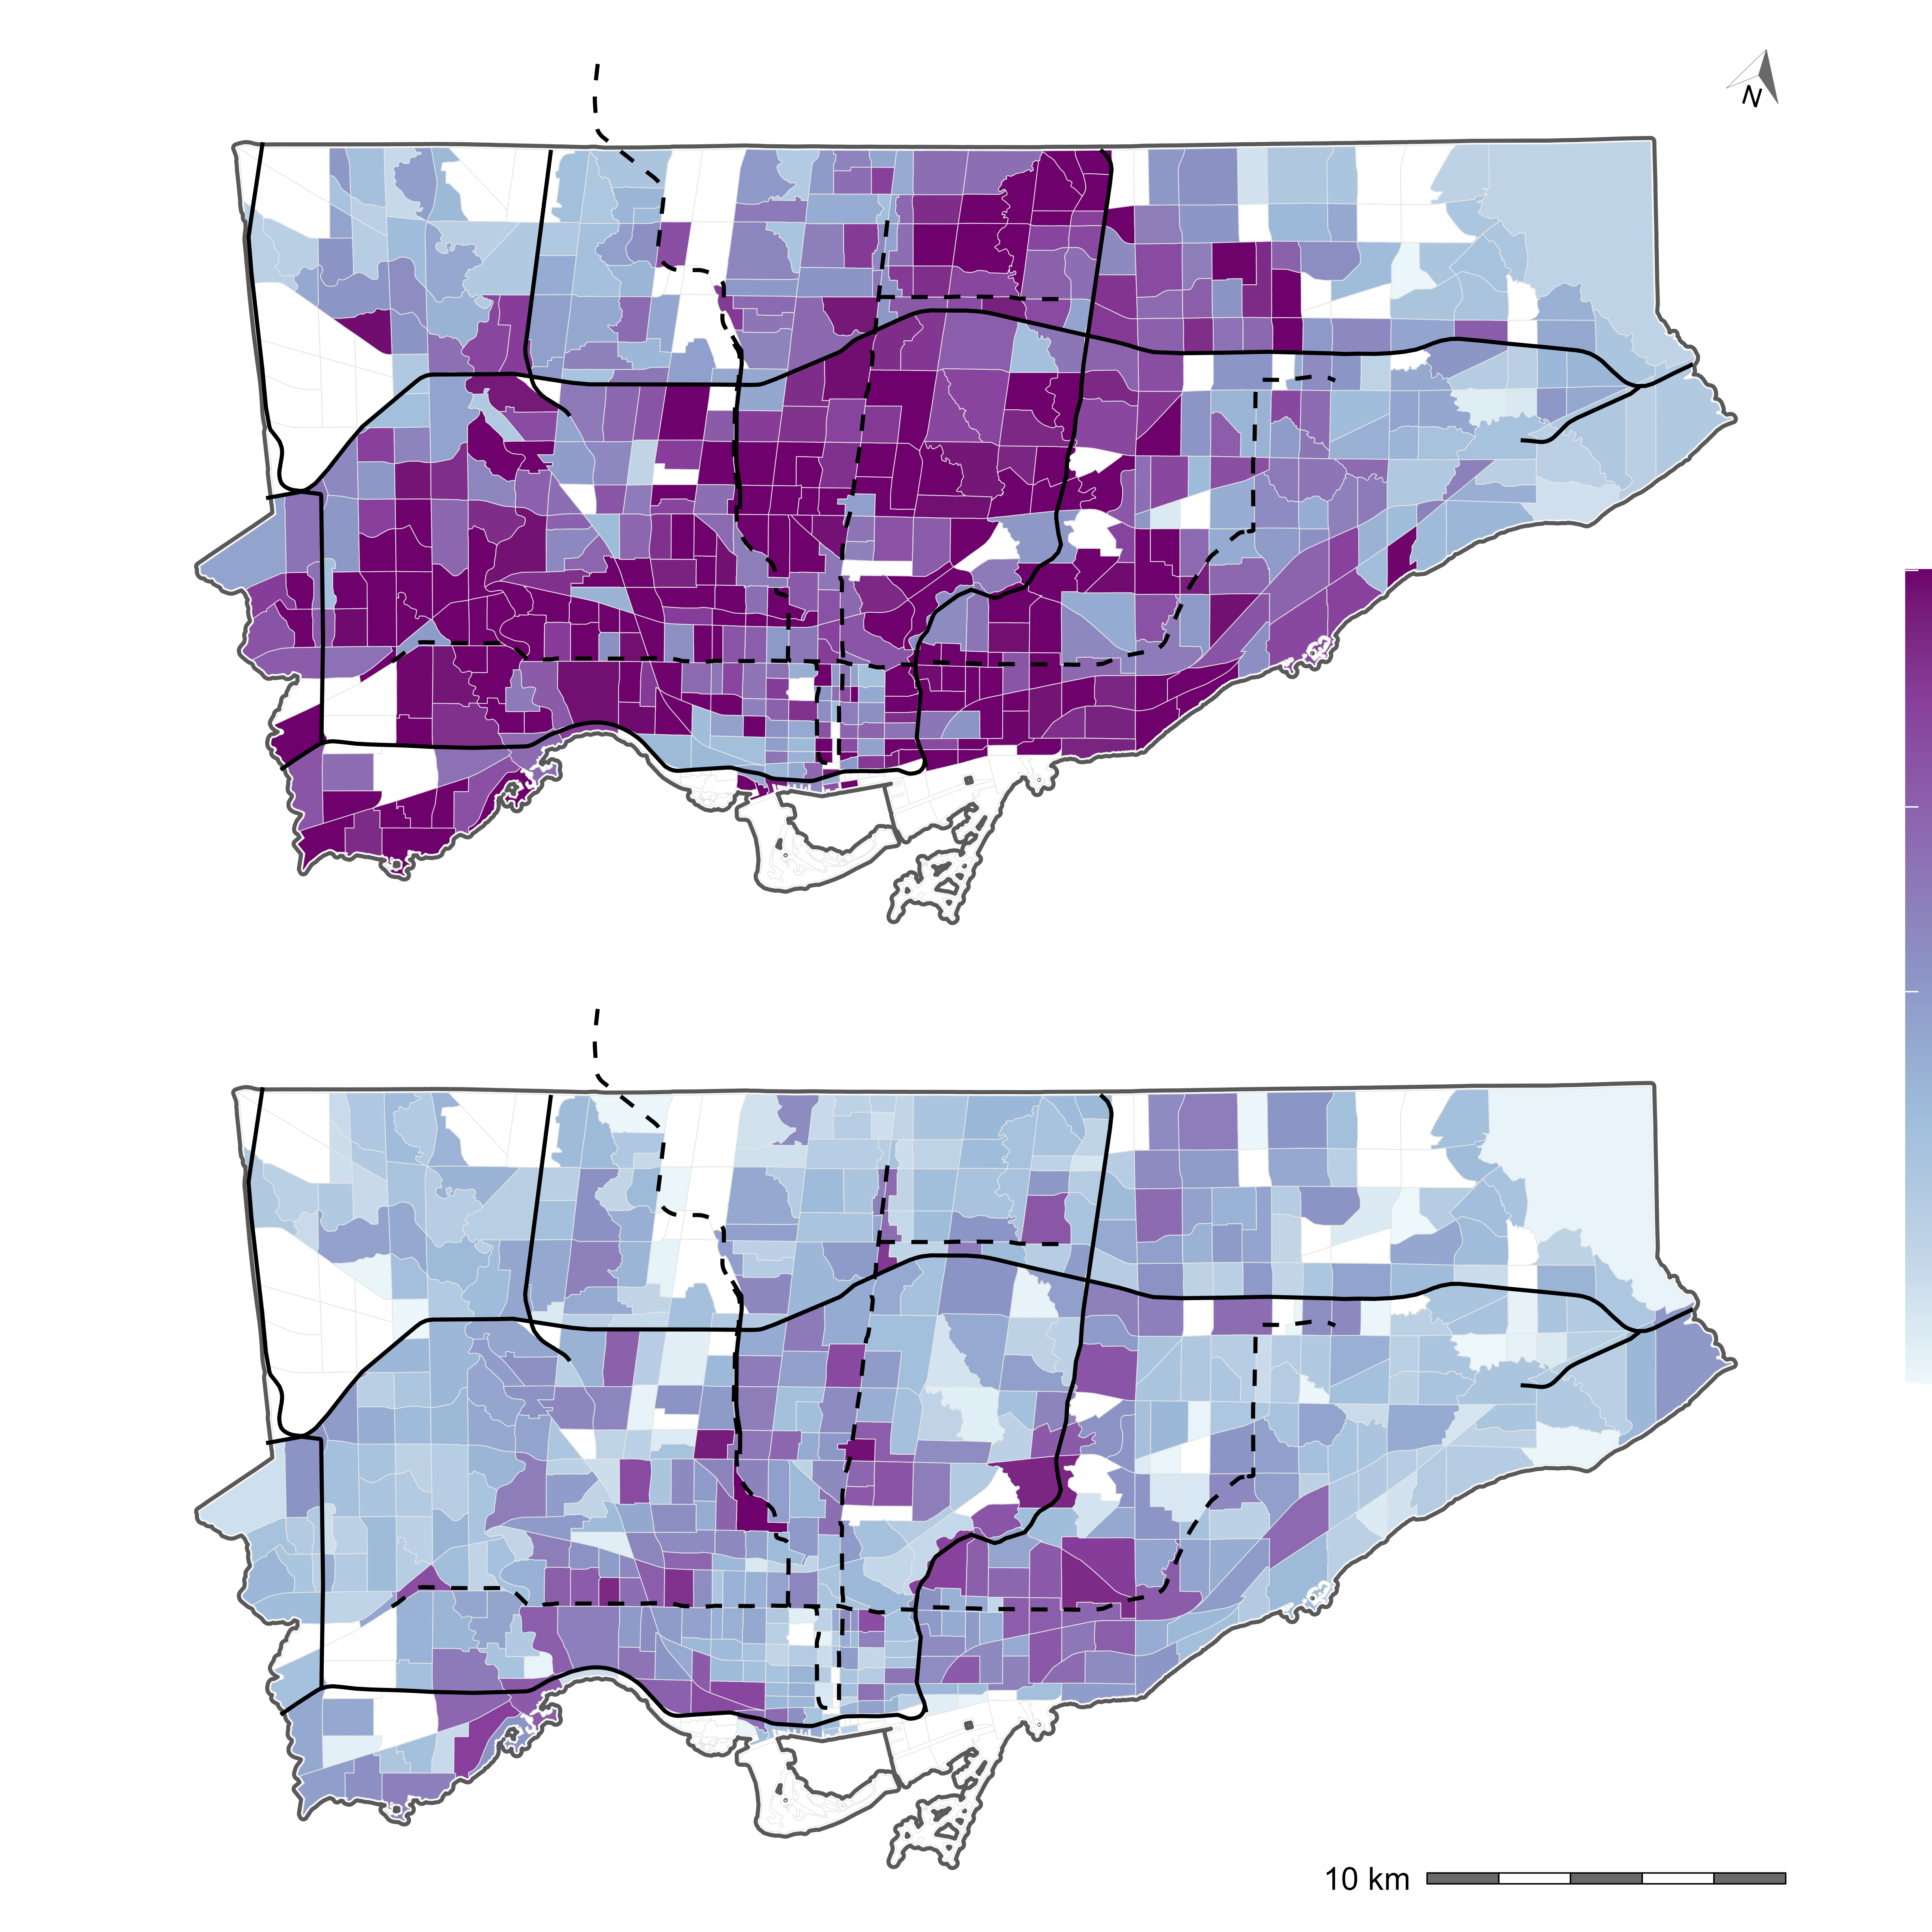
\includegraphics[width=1\linewidth]{images/access-job-Toronto-plot-rates} \caption{\label{fig:rate-accessibility-plot}Hansen-type accessible jobs per capita (top), number of jobs to population ratio (middle), and spatially available jobs per capita (bottom) for Toronto. The city benchmark corresponds to total number of jobs in Toronto divided by the number of workers in Toronto, since this is equal the value is 1. Black lines represent expressways and black dashed lines represent subway lines. All white TAZ have no worker population or jobs, i.e., with null accessibility values.}\label{fig:rate-accessibility-plot}
\end{figure}

Figure \ref{fig:rate-accessibility-plot} presents the number of jobs per
capita for Hansen-type accessibility (top plot), the raw number of jobs
per capita (middle plot), and the spatially available jobs per capita
(bottom plot). In addition to clarifying the meaning of internal values,
spatial availability can also be divided by population at each origin
and expressed as a rate: this rate can be used as a benchmark for equity
analysis and compared directly to the raw number of jobs per capita.

The bottom plot features a value which is mathematically equivalent to
Shen-type measure, but with stronger interpretability thanks to the
proportional allocation mechanism. This mechanism makes clear that all
the opportunities are allocated proportionally to origins, which
improves interpretability since the \(V_i\) values are the absolute
value of \emph{opportunity availability}. The value can thus can be
directly divided by the population at the origin and expressed as
opportunities per capita. When spatial availability is compared to
Hansen-type measure (top plot), dividing the output by population
directly yield's a more difficult to interpret number of
\emph{unconstrained} accessible jobs per capita. For instance, the
median light-pink shaded TAZ corresponds to approximately 5.89
unconstrained accessible jobs per capita; this value is difficult to
intercept, because as discussed in the introduction, jobs are
\emph{exclusive} opportunity types so their accessibility value should
take into consideration competition.

The bottom plot displays the spatially available jobs per capita. It can
be interpreted as a benchmark its values can be compared directly to the
raw number of jobs per capita (middle plot) since the total number of
opportunities are preserved (and the population, in this case, is
equivalent to the number of opportunities). For instance, a TAZ with a
\(v_i > 1\) have more \emph{available jobs} (based on travel behaviour
and competition) than their working population. This TA has sufficient
employment opportunities (under the assumptions of the input data),
while TAZ with a \(v_i < 1\) do not have sufficient employment
opportunities. From an equity perspective, \(v_i\) can be used to target
where residential housing, job opportunities, and/or transportation
system improvements should be created. For TAZ with \(v_i\) values
significantly greater than 1 (dark pinks), constructing more residential
housing for the type of workers who occupy the \emph{available jobs} in
the proximate TAZ should be considered. Assuming the input data is
correct, increasing the competition in the area will decrease the
\(v_i\) score but if can be decreased up to threshold of \(v_i = 1\).
For TAZ with \(v_i\) values significantly less than 1 (light pinks),
constructing more employment opportunities for the type of workers who
live in proximate TAZ and/or prioritizing transportation network
improvements to create more favourable travel time conditions. Depending
on the raw jobs per worker ratio, different approaches are appropriate.
For instance, adding more residential locations near the downtown core
(bottom center on the bottom plot) could be a good approach to
increasing \(v_i\) as there is already a high jobs per worker ratio
(middle plot). However, doing so will decrease the \(v_i\) availability
in areas near the border of the city, so in addition to doing so, adding
more employment opportunities to areas with low raw jobs per worker
ratio and low \(v_i\) is needed. In addition to these changes, the
travel time landscape would also influence the resulting \(v_i\) score,
so transportation network improves to areas with low \(v_i\) could also
be considered. This is to say, \(v_i\) is dependent on the magnitude and
spatial distribution of residential housing, job opportunities, and
transportation system so the region could be optimized to achieve
thresholds of specific \(v_i\) values and thus the difference in
residential housing, job opportunities, and transportation system can
become policy targets. It should also be kept in mind, that though
\(v_i = 1\) and the comparison to the raw jobs per worker values can be
used for policy planning, \(v_i\) can easily be transformed back to
\(V_i\) to understand the magnitude of the job availability within that
origin.

\newpage

\hypertarget{conclusion}{%
\section{Conclusion}\label{conclusion}}

In this paper we show how a widely used measure of accessibility with
competition (Shen-type accessibility) obscures some important internal
values of opportunities taken. This is caused by confounding the
population of zones with the \emph{effective opportunity-seeking
population}. We then propose an alternative derivation of accessibility
with competition that we call spatial availability. This measure ensures
that opportunities are allocated in a proportional way and preserved in
the regional total. We also show that spatial availability and Shen-type
accessibility are equifinal: formally the equations are the same (along
with 2SFCA) and can be consider as singly-constrained measures.

Spatial availability matters because competition is an important
consideration for certain opportunity types and conventional Hansen-type
accessibility does not capture it {[}25{]}. Spatial availability also
brings forward a different interpretation to competition than the
Shen-type measure through its intermediate values. In equity analysis
and policy planning, an analyst might be interested in the internal
values of their accessibility analysis, for example travel times, and
who pays how much for accessibility. The increased interpretability and
internal consistency of spatial availability can help to push
accessibility analysis forward. Hansen-type measure tends to result in
values which are very extreme as a result of multiple-counting
opportunities as shown in empirical example. Multiple-counting may not
be an issue if the opportunity-type is non-exclusive, but with the case
of employment where one worker can only take one job, the resulting
values are difficult to interpret (though it can be interpreted
relatively to speak about urban form). In this paper, we also
demonstrated how attempting to disentangle the absolute values of
opportunities from the Shen-type measure is difficult as a result of
Shen's definition which confounds the population with the
effective-opportunity seeking population.

As demonstrated in this paper, spatial availability increases
interpretability by first presenting the absolute value of
\emph{available} jobs and then by dividing the available jobs value by
the number of working population. This rate is equivalent to Shen-type
measure but contains internal values, such as the proportional
allocation mechanism, that yield more realistic estimates of
opportunities taken, as well as a set of balancing factors that can be
used to better understand the absolute and rate values obtained.

Based on the research presented, we suggest the following guidelines for
the application of spatial availability and the topic of future work:

\begin{enumerate}
\def\labelenumi{\arabic{enumi})}
\item
  The Hansen-style accessibility should be used when opportunities are
  non-exclusive. When opportunities are perfectly exclusive (i.e., 1
  spot for 1 person), spatial availability (i.e., accessibility with
  competition) should be used.
\item
  Shen-type accessibility can be used to compute the availability of
  jobs (the rate and the absolute values if the original definition is
  corrected), however, if the analyst is interested in internal values
  and secondary analysis of the results, spatial availability should be
  considered.
\item
  With the renewed interpretability of what the absolute
  \emph{opportunity availability} is at each origin, the spatial
  availability per capita \(v_i\) value of 1 can be used as a policy
  goal. For areas with a value below 1, targeted increases to the
  quantity of opportunities, residential housing, and transportation
  system improvements can be considered such that the number of
  \emph{available jobs} per capita in the zone is at least equal to 1.
  Since spatial availability per capita implicitly preserves the number
  of opportunities in the region, it can be directly compared to the the
  region's raw jobs to population ratio to inform policy. Additionally,
  the absolute values of spatial availability can be used to understand
  the magnitude of the opportunity availability deficit (or surplus).
\item
  Spatial availability per capita can also be compared directly to other
  regions as done by literature using Shen-type measure/2SFCA (e.g.,
  {[}64{]}; {[}65{]}; {[}66{]}). However, as a result of the renewed
  interpretation, the magnitude of \emph{spatially available}
  opportunities can be quantified.
\item
  Lastly, since opportunities are preserved, many new avenues of
  analysis can be pursued. This is especially important in light of
  emerging concerns with equity. For instance, the population and
  opportunities can be segmented (i.e., transit users, active
  transportation users, low income, low education, new comers, children)
  and their spatial availability to opportunities can be assessed,
  benchmarked, and corresponding policy to target inequities can be
  theorized. As another example, the combined balancing factor can be
  analysed to identify which populations currently do not seek
  opportunities because of friction of distance.
\end{enumerate}

\begin{landscape}

\section{Appendix A}

The mathematical equivalence of Shen-type accessibility measure and spatial availability is provided in 4 steps in this appendix. Spatial availability per population $v_i$ is solved for population center $A$ (Shen's synthetic example as discussed in Section 2.3): this value is represented by $v_A$ and is equivalent to $a_A$ as follows.

\textbf{First step}: the population-based balancing factor $F^p_{i}$ used in $V_i$ is defined as:
$$
F^p_{i} = \frac{P_{i}^\alpha}{\sum_{i}^N P_{i}^\alpha}
$$

For population center $A$, $F^p_{i}$ is equal to:
$$
F^p_{A} = \frac{P_{A}^\alpha}{P_{A}^\alpha + P_{B}^\alpha + P_{C}^\alpha}
$$

\textbf{Second step}: the impedance-based balancing factor $F^c_{ij}$ in $V_i$ is defined as:
$$
F^c_{ij} = \frac{f(c_{ij})}{\sum_{i=A}^N f(c_{ij})}
$$

In this synthetic example, combinations of workers from population center $A$ are permitted to go to all employment centers ($1$, $2$, $3$), so their relative impedance value is experienced in all of the nine origin-destination trip combinations. Therefore, all nine $F^c_{ij}$ are computed as follows, since they all consider the impact of population center $A$ trip combinations (i.e., either $A1$, $A2$, $A3$).
$$
F^c_{A1} = \frac{f(c_{A1})}{f(c_{A1})+f(c_{B1})+f(c_{C1})}
$$

$$
F^c_{B1} = \frac{f(c_{B1})}{f(c_{A1})+f(c_{B1})+f(c_{C1})}
$$

$$
F^c_{C1} = \frac{f(c_{C1})}{f(c_{A1})+f(c_{B1})+f(c_{C1})}
$$

$$
F^c_{A2} = \frac{f(c_{A2})}{f(c_{A2})+f(c_{B2})+f(c_{C2})}
$$

$$
F^c_{B2} = \frac{f(c_{B2})}{f(c_{A2})+f(c_{B2})+f(c_{C2})}
$$

$$
F^c_{C2} = \frac{f(c_{C2})}{f(c_{A2})+f(c_{B2})+f(c_{C2})}
$$

$$
F^c_{A3} = \frac{f(c_{A3})}{f(c_{A3})+f(c_{B3})+f(c_{C3})}
$$

$$
F^c_{B3} = \frac{f(c_{B3})}{f(c_{A3})+f(c_{B3})+f(c_{C3})}
$$

$$
F^c_{C3} = \frac{f(c_{C3})}{f(c_{A3})+f(c_{B3})+f(c_{C3})}
$$

\textbf{Third step}: when these balancing factors ($F^p_{i}$ and $F^c_{ij}$) concerning population center $A$ are assembled and divided by $P_i$ allow the denominators of the denominators to cancel out. The following equation is the assigned general form, with the strike-through indicating which values cancel out:
$$
v_{i} = \sum_{j}\frac{O_j}{P_{i }^\alpha}\frac{\frac{P_{i}^\alpha}{\cancel{\sum_{i}^N P_{i}^\alpha}} \cdot \frac{f(c_{ij})}{\cancel{\sum_{i}^N f(c_{ij})}}}{\sum_{i}^N \frac{P_{i}^\alpha}{\cancel{\sum_{i}^N P_{i}^\alpha}} \cdot \frac{f(c_{ij})}{\cancel{\sum_{i}^N f(c_{ij})}}}\
$$

To demonstrate that those denominator terms cancel out, the following following terms for $v_A$ are subbed into the general form as follows:
$$
v_{A} = \frac{O_1}{P_{A}^\alpha}(\frac{\frac{P_{A}^\alpha}{P_{A}^\alpha+P_{B}^\alpha+P_{C}^\alpha} \cdot \frac{f(c_{A1})}{f(c_{A1})+f(c_{B1})+f(c_{C1})}}{\frac{P_{A}^\alpha}{P_{A}^\alpha+P_{B}^\alpha+P_{C}^\alpha} \cdot \frac{f(c_{A1})}{f(c_{A1})+f(c_{B1})+f(c_{C1})} + \frac{P_{A}^\alpha}{P_{A}^\alpha+P_{B}^\alpha+P_{C}^\alpha} \cdot \frac{f(c_{B1})}{f(c_{A1})+f(c_{B1})+f(c_{C1})}+ \frac{P_{A}^\alpha}{P_{A}^\alpha+P_{B}^\alpha+P_{C}^\alpha} \cdot \frac{f(c_{C1})}{f(c_{A1})+f(c_{B1})+f(c_{C1})}}) +
$$

$$
\frac{O_2}{P_{A}^\alpha}(\frac{\frac{P_{A}^\alpha}{P_{A}^\alpha+P_{B}^\alpha+P_{C}^\alpha} \cdot \frac{f(c_{A2})}{f(c_{A2})+f(c_{B2})+f(c_{C2})}}{\frac{P_{A}^\alpha}{P_{A}^\alpha+P_{B}^\alpha+P_{C}^\alpha} \cdot \frac{f(c_{A2})}{f(c_{A2})+f(c_{B2})+f(c_{C2})} + \frac{P_{A}^\alpha}{P_{A}^\alpha+P_{B}^\alpha+P_{C}^\alpha} \cdot \frac{f(c_{B2})}{f(c_{A2})+f(c_{B2})+f(c_{C2})}+\frac{P_{A}^\alpha}{P_{A}^\alpha+P_{B}^\alpha+P_{C}^\alpha} \cdot \frac{f(c_{C2})}{f(c_{A2})+f(c_{B2})+f(c_{C2})}} )+
$$

$$
\frac{O_3}{P_{A}^\alpha}(\frac{\frac{P_{A}^\alpha}{P_{A}^\alpha+P_{B}^\alpha+P_{C}^\alpha} \cdot \frac{f(c_{A3})}{f(c_{A3})+f(c_{B3})+f(c_{C3})}}{\frac{P_{A}^\alpha}{P_{A}^\alpha+P_{B}^\alpha+P_{C}^\alpha} \cdot \frac{f(c_{A3})}{f(c_{A3})+f(c_{B3})+f(c_{C3})} + \frac{P_{A}^\alpha}{P_{A}^\alpha+P_{B}^\alpha+P_{C}^\alpha} \cdot \frac{f(c_{B3})}{f(c_{A3})+f(c_{B3})+f(c_{C3})}+\frac{P_{A}^\alpha}{P_{A}^\alpha+P_{B}^\alpha+P_{C}^\alpha} \cdot \frac{f(c_{C3})}{f(c_{A3})+f(c_{B3})+f(c_{C3})}} )
$$

$v_A$ simplifies to the following:
$$
v_{A} = \frac{O_1}{P_{A}^\alpha}(\frac{\frac{P_{A}^\alpha}{P_{A}^\alpha+P_{B}^\alpha+P_{C}^\alpha} \cdot \frac{f(c_{A1})}{f(c_{A1})+f(c_{B1})+f(c_{C1})}}{\frac{P_{A}^\alpha \cdot f(c_{A1}) + P_{A}^\alpha \cdot f(c_{B1}) + P_{A}^\alpha \cdot f(c_{C1})}{(P_{A}^\alpha+P_{B}^\alpha+P_{C}^\alpha) \cdot (f(c_{A1})+f(c_{B1})+f(c_{C1}))}}) +
\frac{O_2}{P_{A}^\alpha}(\frac{\frac{P_{A}^\alpha}{P_{A}^\alpha+P_{B}^\alpha+P_{C}^\alpha} \cdot \frac{f(c_{A2})}{f(c_{A2})+f(c_{B2})+f(c_{C2})}}{\frac{P_{A}^\alpha \cdot f(c_{A2}) + P_{A}^\alpha \cdot f(c_{B2}) + P_{A}^\alpha \cdot f(c_{C2})}{(P_{A}^\alpha+P_{B}^\alpha+P_{C}^\alpha) \cdot (f(c_{A2})+f(c_{B2})+f(c_{C2}))}}) + \frac{O_3}{P_{A}^\alpha}(\frac{\frac{P_{A}^\alpha}{P_{A}^\alpha+P_{B}^\alpha+P_{C}^\alpha} \cdot \frac{f(c_{A3})}{f(c_{A3})+f(c_{B3})+f(c_{C3})}}{\frac{P_{A}^\alpha \cdot f(c_{A3}) + P_{A}^\alpha \cdot f(c_{B3}) + P_{A}^\alpha \cdot f(c_{C3})}{(P_{A}^\alpha+P_{B}^\alpha+P_{C}^\alpha) \cdot (f(c_{A3})+f(c_{B3})+f(c_{C3}))}} )
$$


Now, notice how the denominator of the denominator is the same as the denominator of the numerator for each $j$ (j=1, j=2, and j=3)? We remove those cancelled out terms (as indicated at the beginning of this step) and re-write $v_a$ as follows:
$$
v_{A} = \frac{O_1}{P_{A}^\alpha}(\frac{P_{A}^\alpha \cdot f(c_{A1})}{P_{A}^\alpha \cdot f(c_{A1}) + P_{A}^\alpha \cdot f(c_{B1}) + P_{A}^\alpha \cdot f(c_{C1})} + \frac{O_2}{P_{A}^\alpha}\frac{P_{A}^\alpha \cdot f(c_{A2})}{P_{A}^\alpha \cdot f(c_{A2}) + P_{A}^\alpha \cdot f(c_{B2}) + P_{A}^\alpha \cdot f(c_{C2})} + \frac{O_3}{P_{A}^\alpha}\frac{P_{A}^\alpha \cdot f(c_{A3})}{P_{A}^\alpha \cdot f(c_{A3}) + P_{A}^\alpha \cdot f(c_{B3}) + P_{A}^\alpha \cdot f(c_{C3})} )
$$

\textbf{Fourth step}: We can now cancel out one more term, $P_{A}^\alpha$, from the denominator and numerator as follows:
$$
v_{A} = \frac{O_1}{\cancel{P_{A}^\alpha}}(\frac{\cancel{P_{A}^\alpha} \cdot f(c_{A1})}{P_{A}^\alpha \cdot f(c_{A1}) + P_{A}^\alpha \cdot f(c_{B1}) + P_{A}^\alpha \cdot f(c_{C1})} + \frac{O_2}{\cancel{P_{A}^\alpha}}\frac{\cancel{P_{A}^\alpha} \cdot f(c_{A2})}{P_{A}^\alpha \cdot f(c_{A2}) + P_{A}^\alpha \cdot f(c_{B2}) + P_{A}^\alpha \cdot f(c_{C2})} + \frac{O_3}{\cancel{P_{A}^\alpha}}\frac{\cancel{P_{A}^\alpha} \cdot f(c_{A3})}{P_{A}^\alpha \cdot f(c_{A3}) + P_{A}^\alpha \cdot f(c_{B3}) + P_{A}^\alpha \cdot f(c_{C3})} )
$$

Which can be expressed as: 
$$
v_{A} = (\frac{O_1 \cdot f(c_{A1})}{P_{A}^\alpha \cdot f(c_{A1}) + P_{B}^\alpha \cdot f(c_{B1}) + P_{C}^\alpha \cdot f(c_{C1})} + \frac{O_2  \cdot f(c_{A2})}{P_{A}^\alpha \cdot f(c_{A2}) + P_{B}^\alpha \cdot f(c_{B2}) + P_{C}^\alpha \cdot f(c_{C2})} + \frac{O_3 \cdot f(c_{A3})}{P_{A}^\alpha \cdot f(c_{A3}) + P_{B}^\alpha \cdot f(c_{B3}) + P_{C}^\alpha \cdot f(c_{C3})} )
$$
And generalized to be formally identical to the Shen-type accessibility measure with competition as follows:
$$
v_{i} = {a_i} = \sum_j{\frac{O_j \cdot f(c_{ij})}{\sum_i P_{i} \cdot f(c_{ij})}}
$$\\


\end{landscape}

\textbackslash end\{landscape\}

\section{References}

\hypertarget{refs}{}
\begin{CSLReferences}{0}{0}
\leavevmode\vadjust pre{\hypertarget{ref-hansen1959}{}}%
\CSLLeftMargin{1. }%
\CSLRightInline{Hansen WG. How Accessibility Shapes Land Use. Journal of
the American Institute of Planners. 1959;25: 73--76.
doi:\href{https://doi.org/10.1080/01944365908978307}{10.1080/01944365908978307}}

\leavevmode\vadjust pre{\hypertarget{ref-handy_measuring_1997}{}}%
\CSLLeftMargin{2. }%
\CSLRightInline{Handy SL, Niemeier DA. Measuring {Accessibility}: {An}
{Exploration} of {Issues} and {Alternatives}. Environment and Planning
A: Economy and Space. 1997;29: 1175--1194.
doi:\href{https://doi.org/10.1068/a291175}{10.1068/a291175}}

\leavevmode\vadjust pre{\hypertarget{ref-shi_literature_2020}{}}%
\CSLLeftMargin{3. }%
\CSLRightInline{Shi Y, Blainey S, Sun C, Jing P. A literature review on
accessibility using bibliometric analysis techniques. Journal of
Transport Geography. 2020;87: 102810.
doi:\href{https://doi.org/10.1016/j.jtrangeo.2020.102810}{10.1016/j.jtrangeo.2020.102810}}

\leavevmode\vadjust pre{\hypertarget{ref-deboosere2018}{}}%
\CSLLeftMargin{4. }%
\CSLRightInline{Deboosere R, El-Geneidy AM, Levinson D.
Accessibility-oriented development. Journal of Transport Geography.
2018;70: 11--20.
doi:\href{https://doi.org/10.1016/j.jtrangeo.2018.05.015}{10.1016/j.jtrangeo.2018.05.015}}

\leavevmode\vadjust pre{\hypertarget{ref-handy2020}{}}%
\CSLLeftMargin{5. }%
\CSLRightInline{Handy S. Is accessibility an idea whose time has finally
come? Transportation Research Part D: Transport and Environment.
2020;83: 102319.
doi:\href{https://doi.org/10.1016/j.trd.2020.102319}{10.1016/j.trd.2020.102319}}

\leavevmode\vadjust pre{\hypertarget{ref-proffitt2017}{}}%
\CSLLeftMargin{6. }%
\CSLRightInline{Proffitt DG, Bartholomew K, Ewing R, Miller HJ.
Accessibility planning in American metropolitan areas: Are we there yet?
Urban Studies. 2017;56: 167--192.
doi:\href{https://doi.org/10.1177/0042098017710122}{10.1177/0042098017710122}}

\leavevmode\vadjust pre{\hypertarget{ref-yan2021}{}}%
\CSLLeftMargin{7. }%
\CSLRightInline{Yan X. Toward Accessibility-Based Planning. Journal of
the American Planning Association. 2021;87: 409--423.
doi:\href{https://doi.org/10.1080/01944363.2020.1850321}{10.1080/01944363.2020.1850321}}

\leavevmode\vadjust pre{\hypertarget{ref-harris_market_1954}{}}%
\CSLLeftMargin{8. }%
\CSLRightInline{Harris CD. The {Market} as a {Factor} in the
{Localization} of {Industry} in the {United} {States}. Annals of the
Association of American Geographers. 1954;44: 315--348. Available:
\url{https://www.jstor.org/stable/2561395}}

\leavevmode\vadjust pre{\hypertarget{ref-wilson1971}{}}%
\CSLLeftMargin{9. }%
\CSLRightInline{Wilson AG. A Family of Spatial Interaction Models, and
Associated Developments. Environment and Planning A: Economy and Space.
1971;3: 1--32.
doi:\href{https://doi.org/10.1068/a030001}{10.1068/a030001}}

\leavevmode\vadjust pre{\hypertarget{ref-cervero_transportation_2002}{}}%
\CSLLeftMargin{10. }%
\CSLRightInline{Cervero R, Sandoval O, Landis J. Transportation as a
{Stimulus} of {Welfare}-to-{Work}: {Private} versus {Public} {Mobility}.
Journal of Planning Education and Research. 2002;22: 50--63.
doi:\href{https://doi.org/10.1177/0739456X0202200105}{10.1177/0739456X0202200105}}

\leavevmode\vadjust pre{\hypertarget{ref-paez2004network}{}}%
\CSLLeftMargin{11. }%
\CSLRightInline{Paez A. Network accessibility and the spatial
distribution of economic activity in eastern asia. Urban Studies.
2004;41: 2211--2230. }

\leavevmode\vadjust pre{\hypertarget{ref-geurs2004}{}}%
\CSLLeftMargin{12. }%
\CSLRightInline{Geurs KT, van Wee B. Accessibility evaluation of
land-use and transport strategies: review and research directions.
Journal of Transport Geography. 2004;12: 127--140.
doi:\href{https://doi.org/10.1016/j.jtrangeo.2003.10.005}{10.1016/j.jtrangeo.2003.10.005}}

\leavevmode\vadjust pre{\hypertarget{ref-levinson_accessibility_1998}{}}%
\CSLLeftMargin{13. }%
\CSLRightInline{Levinson DM. Accessibility and the journey to work.
Journal of Transport Geography. 1998;6: 11--21.
doi:\href{https://doi.org/10.1016/S0966-6923(97)00036-7}{10.1016/S0966-6923(97)00036-7}}

\leavevmode\vadjust pre{\hypertarget{ref-Arranz2019measuring}{}}%
\CSLLeftMargin{14. }%
\CSLRightInline{Arranz-López A, Soria-Lara JA, Witlox F, Páez A.
Measuring relative non-motorized accessibility to retail activities.
International Journal of Sustainable Transportation. 2019;13: 639--651.
doi:\href{https://doi.org/10.1080/15568318.2018.1498563}{10.1080/15568318.2018.1498563}}

\leavevmode\vadjust pre{\hypertarget{ref-yangStudyImpactHighSpeed2018}{}}%
\CSLLeftMargin{15. }%
\CSLRightInline{Yang J, Guo A, Li X, Huang T. Study of the {Impact} of a
{High-Speed Railway Opening} on {China}'s {Accessibility Pattern} and
{Spatial Equality}. Sustainability. 2018;10: 2943.
doi:\href{https://doi.org/10.3390/su10082943}{10.3390/su10082943}}

\leavevmode\vadjust pre{\hypertarget{ref-miller2018}{}}%
\CSLLeftMargin{16. }%
\CSLRightInline{Miller EJ. Accessibility: measurement and application in
transportation planning. Transport Reviews. 2018;38: 551--555.
doi:\href{https://doi.org/10.1080/01441647.2018.1492778}{10.1080/01441647.2018.1492778}}

\leavevmode\vadjust pre{\hypertarget{ref-allen2019}{}}%
\CSLLeftMargin{17. }%
\CSLRightInline{Allen J, Farber S. A Measure of Competitive Access to
Destinations for Comparing Across Multiple Study Regions. Geographical
Analysis. 2019;52: 69--86.
doi:\href{https://doi.org/10.1111/gean.12188}{10.1111/gean.12188}}

\leavevmode\vadjust pre{\hypertarget{ref-paez_healthcare_2010}{}}%
\CSLLeftMargin{18. }%
\CSLRightInline{Páez A, Mercado R, Farber S, Morency C, Roorda M.
Accessibility to health care facilities in montreal island: An
application of relative accessibility indicators from the perspective of
senior and non-senior residents. International Journal of Health
Geographics. 2010;9: 1--9. Available:
\url{http://www.ij-healthgeographics.com/content/9/1/52}}

\leavevmode\vadjust pre{\hypertarget{ref-campbell_2019_accessibility}{}}%
\CSLLeftMargin{19. }%
\CSLRightInline{Campbell KB, Rising JA, Klopp JM, Mbilo JM.
Accessibility across transport modes and residential developments in
nairobi. Journal of Transport Geography. 2019;74: 77--90.
doi:\href{https://doi.org/10.1016/j.jtrangeo.2018.08.002}{10.1016/j.jtrangeo.2018.08.002}}

\leavevmode\vadjust pre{\hypertarget{ref-bocarejo_s_transport_2012}{}}%
\CSLLeftMargin{20. }%
\CSLRightInline{Bocarejo S. JP, Oviedo H. DR. Transport accessibility
and social inequities: A tool for identification of mobility needs and
evaluation of transport investments. Journal of Transport Geography.
2012;24: 142--154.
doi:\href{https://doi.org/10.1016/j.jtrangeo.2011.12.004}{10.1016/j.jtrangeo.2011.12.004}}

\leavevmode\vadjust pre{\hypertarget{ref-elgeneidy_cost_2016}{}}%
\CSLLeftMargin{21. }%
\CSLRightInline{El-Geneidy A, Levinson D, Diab E, Boisjoly G, Verbich D,
Loong C. The cost of equity: {Assessing} transit accessibility and
social disparity using total travel cost. Transportation Research Part
A: Policy and Practice. 2016;91: 302--316.
doi:\href{https://doi.org/10.1016/j.tra.2016.07.003}{10.1016/j.tra.2016.07.003}}

\leavevmode\vadjust pre{\hypertarget{ref-jiang_2016_accessibility}{}}%
\CSLLeftMargin{22. }%
\CSLRightInline{Jiang H, Levinson DM. Accessibility and the evaluation
of investments on the beijing subway. Journal of Transport and Land Use.
2016;10.
doi:\href{https://doi.org/10.5198/jtlu.2016.884}{10.5198/jtlu.2016.884}}

\leavevmode\vadjust pre{\hypertarget{ref-hu_2019_measuring}{}}%
\CSLLeftMargin{23. }%
\CSLRightInline{Hu Y, Downs J. Measuring and visualizing place-based
space-time job accessibility. Journal of Transport Geography. 2019;74:
278--288.
doi:\href{https://doi.org/10.1016/j.jtrangeo.2018.12.002}{10.1016/j.jtrangeo.2018.12.002}}

\leavevmode\vadjust pre{\hypertarget{ref-kelobonye2020measuring}{}}%
\CSLLeftMargin{24. }%
\CSLRightInline{Kelobonye K, Zhou H, McCarney G, Xia J. Measuring the
accessibility and spatial equity of urban services under competition
using the cumulative opportunities measure. Journal of Transport
Geography. 2020;85: 102706.
doi:\url{https://doi.org/10.1016/j.jtrangeo.2020.102706}}

\leavevmode\vadjust pre{\hypertarget{ref-merlin2017competition}{}}%
\CSLLeftMargin{25. }%
\CSLRightInline{Merlin LA, Hu L. Does competition matter in measures of
job accessibility? Explaining employment in los angeles. Journal of
Transport Geography. 2017;64: 77--88.
doi:\href{https://doi.org/10.1016/j.jtrangeo.2017.08.009}{10.1016/j.jtrangeo.2017.08.009}}

\leavevmode\vadjust pre{\hypertarget{ref-shen1998}{}}%
\CSLLeftMargin{26. }%
\CSLRightInline{Shen Q. Location characteristics of inner-city
neighborhoods and employment accessibility of low-wage workers.
Environment and Planning B: Planning and Design. 1998;25: 345--365.
doi:\href{https://doi.org/10.1068/b250345}{10.1068/b250345}}

\leavevmode\vadjust pre{\hypertarget{ref-paez2019}{}}%
\CSLLeftMargin{27. }%
\CSLRightInline{Paez A, Higgins CD, Vivona SF. Demand and level of
service inflation in Floating Catchment Area (FCA) methods. Shah TI,
editor. PLOS ONE. 2019;14: e0218773.
doi:\href{https://doi.org/10.1371/journal.pone.0218773}{10.1371/journal.pone.0218773}}

\leavevmode\vadjust pre{\hypertarget{ref-weibull_axiomatic_1976}{}}%
\CSLLeftMargin{28. }%
\CSLRightInline{Weibull JW. An axiomatic approach to the measurement of
accessibility. Regional Science and Urban Economics. 1976;6: 357--379.
doi:\href{https://doi.org/10.1016/0166-0462(76)90031-4}{10.1016/0166-0462(76)90031-4}}

\leavevmode\vadjust pre{\hypertarget{ref-joseph1984}{}}%
\CSLLeftMargin{29. }%
\CSLRightInline{Joseph AE, Bantock PR. Rural Accessibility of General
Practitioners: the Case of Bruce and Grey Counties, ONTARIO,
1901{\textendash}1981. The Canadian Geographer/Le Géographe canadien.
1984;28: 226--239.
doi:\href{https://doi.org/10.1111/j.1541-0064.1984.tb00788.x}{10.1111/j.1541-0064.1984.tb00788.x}}

\leavevmode\vadjust pre{\hypertarget{ref-luo2003}{}}%
\CSLLeftMargin{30. }%
\CSLRightInline{Luo W, Wang F. Measures of Spatial Accessibility to
Health Care in a GIS Environment: Synthesis and a Case Study in the
Chicago Region. Environment and Planning B: Planning and Design.
2003;30: 865--884.
doi:\href{https://doi.org/10.1068/b29120}{10.1068/b29120}}

\leavevmode\vadjust pre{\hypertarget{ref-yang_comparing_2006}{}}%
\CSLLeftMargin{31. }%
\CSLRightInline{Yang D-H, Goerge R, Mullner R. Comparing {GIS}-{Based}
{Methods} of {Measuring} {Spatial} {Accessibility} to {Health}
{Services}. Journal of Medical Systems. 2006;30: 23--32.
doi:\href{https://doi.org/10.1007/s10916-006-7400-5}{10.1007/s10916-006-7400-5}}

\leavevmode\vadjust pre{\hypertarget{ref-chen_spatial_2020}{}}%
\CSLLeftMargin{32. }%
\CSLRightInline{Chen Z, Zhou X, Yeh AG. Spatial accessibility to
kindergartens using a spectrum combinational approach: {Case} study of
{Shanghai} using cellphone data. Environment and Planning B: Urban
Analytics and City Science. 2020; 239980832095422.
doi:\href{https://doi.org/10.1177/2399808320954221}{10.1177/2399808320954221}}

\leavevmode\vadjust pre{\hypertarget{ref-ye_spatial_2018}{}}%
\CSLLeftMargin{33. }%
\CSLRightInline{Ye C, Zhu Y, Yang J, Fu Q. Spatial equity in accessing
secondary education: {Evidence} from a gravity-based model: {Spatial}
equity in accessing secondary education. The Canadian Geographer / Le
Géographe canadien. 2018;62: 452--469.
doi:\href{https://doi.org/10.1111/cag.12482}{10.1111/cag.12482}}

\leavevmode\vadjust pre{\hypertarget{ref-chen_enhancing_2019}{}}%
\CSLLeftMargin{34. }%
\CSLRightInline{Chen X. Enhancing the {Two}-{Step} {Floating}
{Catchment} {Area} {Model} for {Community} {Food} {Access} {Mapping}:
{Case} of the {Supplemental} {Nutrition} {Assistance} {Program}. The
Professional Geographer. 2019;71: 668--680.
doi:\href{https://doi.org/10.1080/00330124.2019.1578978}{10.1080/00330124.2019.1578978}}

\leavevmode\vadjust pre{\hypertarget{ref-chen_evaluating_2020}{}}%
\CSLLeftMargin{35. }%
\CSLRightInline{Chen BY, Cheng X-P, Kwan M-P, Schwanen T. Evaluating
spatial accessibility to healthcare services under travel time
uncertainty: {A} reliability-based floating catchment area approach.
Journal of Transport Geography. 2020;87: 102794.
doi:\href{https://doi.org/10.1016/j.jtrangeo.2020.102794}{10.1016/j.jtrangeo.2020.102794}}

\leavevmode\vadjust pre{\hypertarget{ref-hu_changing_2014}{}}%
\CSLLeftMargin{36. }%
\CSLRightInline{Hu L. Changing {Job} {Access} of the {Poor}: {Effects}
of {Spatial} and {Socioeconomic} {Transformations} in {Chicago},
1990--2010. Urban Studies. 2014;51: 675--692.
doi:\href{https://doi.org/10.1177/0042098013492229}{10.1177/0042098013492229}}

\leavevmode\vadjust pre{\hypertarget{ref-tao_investigating_2020}{}}%
\CSLLeftMargin{37. }%
\CSLRightInline{Tao Z, Zhou J, Lin X, Chao H, Li G. Investigating the
impacts of public transport on job accessibility in {Shenzhen}, {China}:
A multi-modal approach. LAND USE POLICY. 2020;99.
doi:\href{https://doi.org/10.1016/j.landusepol.2020.105025}{10.1016/j.landusepol.2020.105025}}

\leavevmode\vadjust pre{\hypertarget{ref-brunsdon2021opening}{}}%
\CSLLeftMargin{38. }%
\CSLRightInline{Brunsdon C, Comber A. Opening practice: Supporting
reproducibility and critical spatial data science. Journal of
Geographical Systems. 2021;23: 477--496.
doi:\href{https://doi.org/10.1007/s10109-020-00334-2}{10.1007/s10109-020-00334-2}}

\leavevmode\vadjust pre{\hypertarget{ref-paez2021open}{}}%
\CSLLeftMargin{39. }%
\CSLRightInline{Páez A. Open spatial sciences: An introduction. Journal
of Geographical Systems. 2021;23: 467--476.
doi:\href{https://doi.org/10.1007/s10109-021-00364-4}{10.1007/s10109-021-00364-4}}

\leavevmode\vadjust pre{\hypertarget{ref-arribas2021Open}{}}%
\CSLLeftMargin{40. }%
\CSLRightInline{Arribas-Bel D, Green M, Rowe F, Singleton A. Open data
products-a framework for creating valuable analysis ready data. Journal
of Geographical Systems. 2021;23: 497--514.
doi:\href{https://doi.org/10.1007/s10109-021-00363-5}{10.1007/s10109-021-00363-5}}

\leavevmode\vadjust pre{\hypertarget{ref-paez2012measuring}{}}%
\CSLLeftMargin{41. }%
\CSLRightInline{Paez A, Scott DM, Morency C. Measuring accessibility:
Positive and normative implementations of various accessibility
indicators. Journal of Transport Geography. 2012;25: 141--153.
doi:\href{https://doi.org/10.1016/j.jtrangeo.2012.03.016}{10.1016/j.jtrangeo.2012.03.016}}

\leavevmode\vadjust pre{\hypertarget{ref-rosik_forecast_2021}{}}%
\CSLLeftMargin{42. }%
\CSLRightInline{Rosik P, Goliszek S, Komornicki T, Duma P. Forecast of
the {Impact} of {Electric} {Car} {Battery} {Performance} and
{Infrastructural} and {Demographic} {Changes} on {Cumulative}
{Accessibility} for the {Five} {Most} {Populous} {Cities} in {Poland}.
Energies. 2021;14: 8350.
doi:\href{https://doi.org/10.3390/en14248350}{10.3390/en14248350}}

\leavevmode\vadjust pre{\hypertarget{ref-qi_decadelong_2018}{}}%
\CSLLeftMargin{43. }%
\CSLRightInline{Qi Y, Fan Y, Sun T, Hu L(Ivy). Decade-long changes in
spatial mismatch in {Beijing}, {China}: {Are} disadvantaged populations
better or worse off? Environment and Planning A: Economy and Space.
2018;50: 848--868.
doi:\href{https://doi.org/10.1177/0308518X18755747}{10.1177/0308518X18755747}}

\leavevmode\vadjust pre{\hypertarget{ref-kwan_spacetime_1998}{}}%
\CSLLeftMargin{44. }%
\CSLRightInline{Kwan M-P. Space-{Time} and {Integral} {Measures} of
{Individual} {Accessibility}: {A} {Comparative} {Analysis} {Using} a
{Point}-based {Framework}. Geographical Analysis. 1998;30: 191--216.
doi:\href{https://doi.org/10.1111/j.1538-4632.1998.tb00396.x}{10.1111/j.1538-4632.1998.tb00396.x}}

\leavevmode\vadjust pre{\hypertarget{ref-vale_influence_2017}{}}%
\CSLLeftMargin{45. }%
\CSLRightInline{Vale DS, Pereira M. The influence of the impedance
function on gravity-based pedestrian accessibility measures: {A}
comparative analysis. Environment and Planning B: Urban Analytics and
City Science. 2017;44: 740--763.
doi:\href{https://doi.org/10.1177/0265813516641685}{10.1177/0265813516641685}}

\leavevmode\vadjust pre{\hypertarget{ref-reggiani_accessibility_2011}{}}%
\CSLLeftMargin{46. }%
\CSLRightInline{Reggiani A, Bucci P, Russo G. Accessibility and
{Impedance} {Forms}: {Empirical} {Applications} to the {German}
{Commuting} {Network}. International Regional Science Review. 2011;34:
230--252.
doi:\href{https://doi.org/10.1177/0160017610387296}{10.1177/0160017610387296}}

\leavevmode\vadjust pre{\hypertarget{ref-li_approach_2020}{}}%
\CSLLeftMargin{47. }%
\CSLRightInline{Li A, Huang Y, Axhausen KW. An approach to imputing
destination activities for inclusion in measures of bicycle
accessibility. Journal of Transport Geography. 2020;82: 102566.
doi:\href{https://doi.org/10.1016/j.jtrangeo.2019.102566}{10.1016/j.jtrangeo.2019.102566}}

\leavevmode\vadjust pre{\hypertarget{ref-higgins2019}{}}%
\CSLLeftMargin{48. }%
\CSLRightInline{Higgins CD. Accessibility toolbox for r and ArcGIS.
Transport Findings. 2019.
doi:\href{https://doi.org/10.32866/8416}{10.32866/8416}}

\leavevmode\vadjust pre{\hypertarget{ref-santanapalacios2022}{}}%
\CSLLeftMargin{49. }%
\CSLRightInline{Santana Palacios M, El-geneidy A. Cumulative versus
Gravity-based Accessibility Measures: Which One to Use? Findings. 2022.
doi:\href{https://doi.org/10.32866/001c.32444}{10.32866/001c.32444}}

\leavevmode\vadjust pre{\hypertarget{ref-barboza_balancing_2021}{}}%
\CSLLeftMargin{50. }%
\CSLRightInline{Barboza MHC, Carneiro MS, Falavigna C, Luz G, Orrico R.
Balancing time: {Using} a new accessibility measure in {Rio} de
{Janeiro}. Journal of Transport Geography. 2021;90: 102924.
doi:\href{https://doi.org/10.1016/j.jtrangeo.2020.102924}{10.1016/j.jtrangeo.2020.102924}}

\leavevmode\vadjust pre{\hypertarget{ref-pereira_distributional_2019}{}}%
\CSLLeftMargin{51. }%
\CSLRightInline{Pereira RHM, Banister D, Schwanen T, Wessel N.
Distributional effects of transport policies on inequalities in access
to opportunities in {Rio} de {Janeiro}. Journal of Transport and Land
Use. 2019;12.
doi:\href{https://doi.org/10.5198/jtlu.2019.1523}{10.5198/jtlu.2019.1523}}

\leavevmode\vadjust pre{\hypertarget{ref-wang_access_2021}{}}%
\CSLLeftMargin{52. }%
\CSLRightInline{Wang S, Wang M, Liu Y. Access to urban parks:
{Comparing} spatial accessibility measures using three {GIS}-based
approaches. Computers, Environment and Urban Systems. 2021;90: 101713.
doi:\href{https://doi.org/10.1016/j.compenvurbsys.2021.101713}{10.1016/j.compenvurbsys.2021.101713}}

\leavevmode\vadjust pre{\hypertarget{ref-ortuzar_2011_modelling}{}}%
\CSLLeftMargin{53. }%
\CSLRightInline{Ortúzar JD, Willumsen LG. Modelling transport. New York:
Wiley; 2011. }

\leavevmode\vadjust pre{\hypertarget{ref-williams_hall_1981}{}}%
\CSLLeftMargin{54. }%
\CSLRightInline{Williams HCWL. Travel demand forecasting: An overview of
theoretical developments. In: Banister DJ, Hall PG, editors. Transport
and public policy planning. Mansell; 1981. }

\leavevmode\vadjust pre{\hypertarget{ref-sarlas_2020_betweenness}{}}%
\CSLLeftMargin{55. }%
\CSLRightInline{Sarlas G, Paez A, Axhausen KW.
Betweenness-accessibility: Estimating impacts of accessibility on
networks. Journal of Transport Geography. 2020;84: 12.
doi:\href{https://doi.org/10.1016/j.jtrangeo.2020.102680}{10.1016/j.jtrangeo.2020.102680}}

\leavevmode\vadjust pre{\hypertarget{ref-data_management_group_tts_2018}{}}%
\CSLLeftMargin{56. }%
\CSLRightInline{Data Management Group. {TTS} - {Transportation}
{Tomorrow} {Survey} 2016. 2018. Available:
\url{http://dmg.utoronto.ca/transportation-tomorrow-survey/tts-introduction}}

\leavevmode\vadjust pre{\hypertarget{ref-r5r_2021}{}}%
\CSLLeftMargin{57. }%
\CSLRightInline{Rafael H. M. Pereira, Marcus Saraiva, Daniel Herszenhut,
Carlos Kaue Vieira Braga, Matthew Wigginton Conway. r5r: Rapid realistic
routing on multimodal transport networks with R5 in r. Findings. 2021.
doi:\href{https://doi.org/10.32866/001c.21262}{10.32866/001c.21262}}

\leavevmode\vadjust pre{\hypertarget{ref-allen_suburbanization_2021}{}}%
\CSLLeftMargin{58. }%
\CSLRightInline{Allen J, Farber S. Suburbanization of {Transport}
{Poverty}. Annals of the American Association of Geographers. 2021;111:
18. }

\leavevmode\vadjust pre{\hypertarget{ref-higgins2021changes}{}}%
\CSLLeftMargin{59. }%
\CSLRightInline{Higgins CD, Páez A, Ki G, Wang J. Changes in
accessibility to emergency and community food services during COVID-19
and implications for low income populations in hamilton, ontario. Social
Science \& Medicine. 2021; 114442.
doi:\href{https://doi.org/10.1016/j.socscimed.2021.114442}{10.1016/j.socscimed.2021.114442}}

\leavevmode\vadjust pre{\hypertarget{ref-lopez_2017_spatial}{}}%
\CSLLeftMargin{60. }%
\CSLRightInline{Lopez FA, Paez A. Spatial clustering of high-tech
manufacturing and knowledge-intensive service firms in the greater
toronto area. Canadian Geographer-Geographe Canadien. 2017;61: 240--252.
doi:\href{https://doi.org/10.1111/cag.12326}{10.1111/cag.12326}}

\leavevmode\vadjust pre{\hypertarget{ref-horbachov_theoretical_2018}{}}%
\CSLLeftMargin{61. }%
\CSLRightInline{Horbachov P, Svichynskyi S. Theoretical substantiation
of trip length distribution for home-based work trips in urban transit
systems. Journal of Transport and Land Use. 2018;11: 593--632.
Available: \url{https://www.jstor.org/stable/26622420}}

\leavevmode\vadjust pre{\hypertarget{ref-batista_estimation_2019}{}}%
\CSLLeftMargin{62. }%
\CSLRightInline{Batista SFA, Leclercq L, Geroliminis N. Estimation of
regional trip length distributions for the calibration of the aggregated
network traffic models. Transportation Research Part B: Methodological.
2019;122: 192--217.
doi:\href{https://doi.org/10.1016/j.trb.2019.02.009}{10.1016/j.trb.2019.02.009}}

\leavevmode\vadjust pre{\hypertarget{ref-fitdistrplus_2015}{}}%
\CSLLeftMargin{63. }%
\CSLRightInline{Delignette-Muller ML, Dutang C. {fitdistrplus}: An {R}
package for fitting distributions. Journal of Statistical Software.
2015;64: 1--34. Available:
\url{https://www.jstatsoft.org/article/view/v064i04}}

\leavevmode\vadjust pre{\hypertarget{ref-giannotti_inequalities_2021}{}}%
\CSLLeftMargin{64. }%
\CSLRightInline{Giannotti M, Barros J, Tomasiello DB, Smith D, Pizzol B,
Santos BM, et al. Inequalities in transit accessibility: {Contributions}
from a comparative study between {Global} {South} and {North}
metropolitan regions. Cities. 2021;109: 103016.
doi:\href{https://doi.org/10.1016/j.cities.2020.103016}{10.1016/j.cities.2020.103016}}

\leavevmode\vadjust pre{\hypertarget{ref-zhouTransportationAccessibilityEvaluation2021}{}}%
\CSLLeftMargin{65. }%
\CSLRightInline{Zhou C, Zhang D, He X. Transportation {Accessibility
Evaluation} of {Educational Institutions Conducting Field Environmental
Education Activities} in {Ecological Protection Areas}: {A Case Study}
of {Zhuhai City}. Sustainability. 2021;13: 9392.
doi:\href{https://doi.org/10.3390/su13169392}{10.3390/su13169392}}

\leavevmode\vadjust pre{\hypertarget{ref-zhangDifferencesAccessibilityPublic2021}{}}%
\CSLLeftMargin{66. }%
\CSLRightInline{Zhang D, Zhang G, Zhou C. Differences in {Accessibility}
of {Public Health Facilities} in {Hierarchical Municipalities} and the
{Spatial Pattern Characteristics} of {Their Services} in {Doumen
District}, {China}. Land. 2021;10: 1249.
doi:\href{https://doi.org/10.3390/land10111249}{10.3390/land10111249}}

\end{CSLReferences}

\nolinenumbers



\end{document}
